\documentclass[mscthesis, 11pt]{usiinfthesis}

\usepackage[utf8]{inputenc} 

\usepackage{listings}
% Load the package with the acronym option
\usepackage[titletoc,page]{appendix}
\usepackage[acronym,toc,automake,makeindex]{glossaries}

% Generate the glossary
\makeglossary
\renewcommand*\glspostdescription{\dotfill}
\renewcommand*\acronymname{ }


\lstdefinelanguage{algebra}
{morekeywords={import,sort,constructors,observers,transformers,axioms,if,
else,end},
sensitive=false,
morecomment=[l]{//s},
}

\title{Simulation of robot swarms for learning\\ communication-aware coordination} %compulsory
%\specialization{Dependable Distributed Systems}%optional
%\subtitle{Subtitle: Reinventing the World} %optional 
\author{Giorgia Adorni} %compulsory
\begin{committee}
\advisor{Dr.}{Alessandro}{Giusti} %compulsory
\coadvisor{Dr.}{Jèrôme}{Guzzi}{} %optional
\end{committee}
\Day{25} %compulsory
\Month{October} %compulsory
\Year{2020} %compulsory, put only the year
\place{Lugano} %compulsory

\dedication{To my beloved} %optional
\openepigraph{Someone said \dots}{Someone} %optional

%\makeindex %optional, also comment out \theindex at the end

\begin{document}
\maketitle %generates the titlepage, this is FIXED

\frontmatter %generates the frontmatter, this is FIXED

\begin{abstract}
\addcontentsline{toc}{chapter}{Abstract}  % added 
\begingroup
\let\clearpage\relax
In recent years, robotics research has dedicated extensive attention to cooperative 
multi-agent problems, in which agents have a common goal that requires them to 
collaborate, and possibly to communicate, to achieve it.
We investigate imitation learning algorithms to address this issue, providing new 
insights and promising solutions. 
These methods learn a controller by observing demonstrations of an expert, such 
as the behaviour of a centralised omniscient controller, which can perceive the 
entire environment, including the state and observations of all agents. 

Performing tasks with complete knowledge of the state of a system is relatively 
easy, but centralised solutions might not be feasible in real scenarios since agents 
do not have direct access to the state but only to their own observations.
%FIXME add input e output * rifrasa
%To overcome this issue, we train end-to-end \glspl{nn}, usually classifiers or 
%regressors, that only exploit local observations and communications, learning 
%decentralised solution via imitation of a centralised control, which indicates the 
%action to be performed.
To overcome this issue, we train end-to-end \glspl{nn}, usually classifiers or 
regressors, that take as input local observations obtained from an omniscient 
centralised controller, in other words the agents' sensor readings, and the 
communications received, producing as output the action to be performed and 
the communication to be transmitted.

In this study, we focus on two different scenarios: distributing the robots in space 
such that they stand at equal distance from each other, and colouring the robots 
in space depending on their position with respect to the others in the group.
Both are examples of cooperative tasks based on the use of a distributed 
controller. While the second cannot be solved without allowing an explicit 
exchange of messages between the agents, in the first one, a communication 
protocol is not necessary, although it may increase performance.

The experiments are run in Enki, a high-performance open-source simulator for 
planar robots, which provides collision detection and limited physics support for 
robots evolving on a flat surface. Moreover, it can simulate groups of robots 
hundreds of times faster than real-time.

%In addition to analysing typical supervised learning approaches, which directly 
%learn a mapping from observations to actions, we concentrate on more 
%challenging situations where the communication is not provided to the network, 
%instead it is a latent variable which has to be inferred.

The results show how applying a communication strategy improves the 
performance of the distributed model, letting it decide which actions to take 
almost as precisely and quickly as the expert controller.
\endgroup
\end{abstract}


\begin{acknowledgements}
\addcontentsline{toc}{chapter}{Acknowledgements}  % added 
\begingroup
\let\clearpage\relax
I would like to thank my supervisors Alessandro Giusti and Jérôme Guzzi for their 
precious advice and help, my family who have never stopped believing in me and 
to Elia who shared with me this extraordinary journey, always encouraging and 
supporting me, despite all the difficulties.

A special thank goes also to Università della Svizzera Italiana and the University of 
Milano–Bicocca for allowing me to take part in this double degree program and 
to all those people who have accompanied me and made this experience special. 

\endgroup
\end{acknowledgements}

\tableofcontents 
\listoffigures %optional
\listoftables %optional


\mainmatter

\newglossaryentry{fig}{
	name={Fig.},
	description={Figure}
}


\newglossaryentry{tab}{
	name={Tab.},
	description={Table}
}

\newglossaryentry{cm}{
	name={cm},
	description={centimetre}
}

\newglossaryentry{s}{
	name={s},
	description={seconds}
}


\newglossaryentry{h}{
	name={h},
	description={hours}
}

\newglossaryentry{cm/s}{
	name={cm/s},
	description={centimeters per second}
}

\newglossaryentry{wrt}{name={wrt},description={with respect to}}

\chapter{Introduction}
\label{chap:intro}


\subsubsection*{Thesis Outline}
\label{subsec:outline}

This thesis is composed of 7 chapters ,whose main points are presented as follows:
\begin{itemize}
	\item Chapter \ref{chap:stateoftheart} summarises the previous research 
	studies on the topic, evaluating the approaches adopted by the authors.
	
	\item Chapter \ref{chap:background} provides some background knowledge 
	needed to properly understand the research contents.
	
	\item Chapter \ref{chap:impl} presents the tools used for the data collection 
	and all the additional frameworks we relied on.
		
	\item Chapter \ref{chap:methods} thoroughly illustrates the methodology used, 
	their benefits and limitations, including also description of the kind of data 
	used and how they are collected. 

	\item Chapter \ref{chap:experiments} explores the analysis conducted and 
	shows evaluation results.	
	
	\item Chapter \ref{chap:concl} address the results of the experiments and 
	concludes the thesis by discussing the implication of our findings, possible fixes 
	and outlines future works.
	
\end{itemize}


\setcounter{chapter}{0}
\chapter{Literature review}
\label{chap:stateoftheart}
This chapter discusses previous research about the topic, providing a brief 
introduction to the approach we adopted.
%, evaluating, in particular, their shortcomings. 

\glsreset{ai}
\glsreset{dl}
\glsreset{rl} 
\glsreset{dnn}

\bigskip
In recent years, the application of \gls{ai} and \gls{dl} techniques to multi-agent 
cooperative problems has become increasingly successful.
Gasser and Huhns, in \emph{Distributed Artificial Intelligence} 
\cite[][]{gasser2014distributed}, have addressed the issue of coordination and 
cooperation among agents with the combination of distributed systems and 
\gls{ai}, a discipline known as \gls{dai}. 

Similarly, Panait and Luke, in their work \emph{Cooperative multi-agent learning: 
The state of the art} \cite[][]{panait2005cooperative}, report that \gls{mal}, the 
application of machine learning to problems involving multiple agents, has 
become a popular approach which deals with unusually large search spaces. 
In addition, they mention three of the most classic techniques used to solve 
cooperative \gls{ma} problems, that are Supervised and Unsupervised Learning, 
and \gls{rl}. These methods are distinguished according to the type of feedback 
provided to the agent: the target output in the first case, no feedback is provided 
in the second, and reward based on the learned output in the last one.

Given these three options, the vast majority of articles in this field used 
reward-based methods to approach \gls{mal} scenarios, in particular \gls{rl}, that 
make they possible to achieve sophisticated goals in complex and uncertain 
environments \cite[][]{oliehoek2012decentralised}. 
However, this technique is notoriously known for being hard, in particular it is 
difficult to design a suitable reward function for the agents to optimise, which 
precisely leads to the desired behaviour in all possible scenarios. This problem is 
further exacerbated in multi-agent settings \cite[][]{hadfield2017inverse, 
oliehoek2012decentralised}.

\gls{irl} addresses this problem by using a given set of expert trajectories to 
derive a reward function under which these are optimal. 
Nevertheless, this technique imposes often unrealistic requirements 
\cite[][]{vsovsic2016inverse}.

\gls{il} is a class of methods that has been successfully applied to a wide range of 
domains in robotics, for example, autonomous driving 
\cite[][]{schaal1999imitation, stepputtis2019imitation}. They aim to overcome the 
issues aforementioned and, unlike reward-based methods, the model 
acquires skills and provides actions to the agents by observing the desired 
behaviour, performed by an expert \cite[][]{song2018multi, zhang2018deep, 
billard2008survey}.
Using this approach the models learn how to extract relevant information from 
the data provided to them, directly learning a mapping from observations to 
actions. 
A more challenging situation occurs when the model also has to infer the 
coordination among agents that is implicit in the demonstrations, using 
unsupervised approaches to imitation.

In this direction, literature suggests that cooperative tasks sometimes cannot be 
solved using only a simple distributed approach, instead it may be necessary to 
allow an explicit exchange of messages between the agents.
In \emph{Multi-agent reinforcement learning: Independent vs. cooperative 
agents} \cite[][]{tan1993multi}, Tan affirms that cooperating learners should use 
communication in a variety of ways in order to improve team performance: they 
can share instantaneous informations as well as episodic experience and learned 
knowledge.
Also Pesce and Montana propose the use of inter-agent communication for 
situations in which the agents can only acquire partial observations and are faced 
with a task requiring coordination and synchronisation skills 
\cite[][]{pesce2019improving}. Their solution consists in an explicit 
communication system that allows agents to exchange messages that are used 
together with local observations to decide which actions to take.

Our work is based on \emph{Learning distributed controllers by backpropagation}
\cite[][]{marcoverna2020}, which proposes an approach in which a distributed 
policy for the agents and a coordination model are learned at the same time. 
This method is based on an important concept introduced in \emph{Coordinated 
multi-agent imitation learning} \cite[][]{le2017coordinated}: the network has the 
ability to autonomously determine the communication protocol.
Likewise, we use imitation learning approaches to solve the problem of 
coordinating multiple agents, introducing a communication protocol, which 
consists in an explicit exchange of messages between the robots. The 
communication is not provided to the network, instead, it is a latent variable 
which has to be inferred.   
The results show the effectiveness of this communication strategy developed, as 
well as an illustration of the different patterns emerging from the tasks.

\chapter{Methodologies}
\label{chap:methods}
\glsreset{rl}
\glsreset{il}

This chapter illustrates the methodology used to approach the development 
process of this work. 
We start by analysing the domain of the problem (Section \ref{sec:MAS}) and 
defining the learning method (Section \ref{sec:imitlrng}), 
We continue with a presentation of the approaches considered (Section 
\ref{sec:approaches}), followed by  a description of the type of data used for this 
purpose and how they are generated (Section \ref{sec:dataset}).
We conclude with a detailed explanation of the controllers used and of the models
implemented (Section \ref{sec:controllersmodel}). 


\section{Multi-agent system}
\label{sec:MAS}

In this work, we investigate collaborative scenarios in a homogeneous \gls{mas}.

In a given simulated \gls{1d} environment, we consider a team of $N$ interacting 
agents, that are assumed to be interchangeable since they have the same physical 
structure and observation capabilities, which collaborate to solve a given common 
goal \cite[][]{stone2000multiagent, vsovsic2016inverse}.

This system, containing agents also called ``swarming agents’’, in principle is an 
extension of a \gls{decpomdp} \cite[][]{oliehoek2012decentralised}, and can be 
formally defined as a tuple $(S, O, A, R, \pi)$, \cite[][]{schaal1999imitation}, 
where:
\begin{itemize}
	\item $S$ is the state of the system, or the set of local states for each agent, 
	composed of all the possible combinations of positions and observations.
	\item $O$ is the set of possible observations for each agent, obtained through 
	sensors.
	\item $A$ is the set of possible actions for each agent.
	\item $R$ is the reward function $S \times A \rightarrow \mathbb{R}$.
	\item $\pi$ is the policy $S \rightarrow A$ which determines the action to 
	execute in a given state for every single agent.
\end{itemize}

As introduced in Chapter \ref{chap:intro}, through the course of this study we 
tackle two \gls{ma} scenarios, in both of them, the agents have a common goal 
that requires them to cooperate to achieve it. 

Three popular approaches used to solve cooperative \gls{ma} problems are 
supervised and unsupervised learning, and \gls{rl}, which are distinguished 
according to the type of feedback provided, that in the first case is the target, in 
the second no feedback are provided, and in the last one is a reward of the 
learned output \cite[][]{panait2005cooperative}.
However, in reward-based methods, is notoriously hard design a suitable reward 
function, able to lead to the right behaviour in all the possible scenarios, even for 
complex tasks \cite[][]{hadfield2017inverse}.
\gls{il} methods can be used to overcome this problem by learning a policy from 
expert demonstrations without access to a reward signal \cite[][]{song2018multi}.

\section{Imitation Learning}
\label{sec:imitlrng}
\glsreset{rl}
\glsreset{il}
\glsreset{nn}

\gls{il} is a class of methods that has been successfully applied to a 
wide range of domains in robotics, for example, the autonomous driving.
Unlike reward-based methods, \gls{il} acquires skills by observing demonstrations 
of the desired behaviour in order to provide a learning signal to the agents 
\cite[][]{zhang2018deep}.

A typical approach to \gls{il}, also called Behavioural Cloning 
\cite[][]{torabi2018behavioral}, is a supervised technique that consists in 
collecting a certain amount of data, corresponding to a sequence of the 
encountered observations and actions performed by a teacher agent which acts 
according to an unknown policy in order to achieve a certain goal.
Then, the demonstrations of the expert’s behaviour are used to learn a controller, 
by training usually a classifier or regressor, that predict behaviour to correctly 
achieve the same goal in a certain environment \cite[][]{stadie2017third, 
ross2011reduction}.
The machine learning model should be able to learn how to extract relevant 
information from the data provided to it, directly learning a mapping from 
observations to actions.

Instead, in an unsupervised approach are collected only the data that corresponds 
to a sequence of the encountered observations performed by a teacher agent, 
and the controller learned should be able to infer the correspondence from 
observations to actions and find a way to accomplish the same task 
\cite[][]{stadie2017third}.
In this case, learning a good model is more challenging since the coordination, 
that is implicit in the demonstrations, has to be inferred as a latent variable 
\cite[][]{le2017coordinated}.

\section{Approaches}
\label{sec:approaches}
Given the two scenarios presented in Chapter \ref{chap:intro}, distributing the 
robots in space such that they stand at equal distance from each other, and the 
colouring of the robots in space depending on their group membership, through 
the course of this study we tackle two \gls{ma} scenarios, in both of them, the 
agents have a common goal that requires them to cooperate to achieve it. 

While both are excellent examples of distributed tasks, they have an important 
difference: the first problem can be solved without using communication, while 
for the second one it is impossible.
A full explanation of how communication works for Thymio II is covered in 
Section \ref{subsec:thymiocomm}.

\subsection{Distributed approach}
\label{subsec:dist}

As already stated, the first task can be accomplished by using a distributed 
approach without communication.
The agents share the same goal: arrange themselves uniformly along the line 
between the two “dead” robots, in such a way they stand at equal distances from 
each other.
This problem represents an example of a cooperative task, for this reason, it will 
be desirable for the agents to cooperate \cite[][]{barrett2017making}. 

On the one hand, when communication is not possible, they can achieve their 
goal without directly interact with each other. 
As stated by Holland in \emph{Multiagent systems: Lessons from social insects and 
collective robotics} \cite[][]{holland1996multiagent}, since the agents exist in the 
same environment, they can affect each other indirectly in several ways.
For instance, they can be sensed from the other robot’s or they can even change 
the state of an agent by applying a force on it, for example, by colliding with it.
In the work of Grassè about Stigmergy Theory are provided additional details 
about active and passive stigmergy \cite[][]{grasse1959reconstruction}.

On the other hand, the difficulty of the problem we do consider is that the agent 
does not have full knowledge of its mates’ behaviours.
Although a communication protocol is not necessary, allows an explicit exchange 
of messages between the agents may nonetheless increase agent performance: 
they use the exchange of message in order to coordinate more effectively and 
distribute more accurately, finally reaching a more efficient solution 
\cite{panait2005cooperative}.

\subsection{Distributed approach with communication}
\label{subsec:comm}

As for the previous task, also in the second the agents share a common goal: 
assuming that they are divided into groups, their objective is to colour themselves 
according to their group membership. 
For this kind of problems, allow explicit communication is not a plus but a 
necessity.

An important aspect that needs to be considered is the decision of what to 
communicate and when so that no issue arises.

Regarding the communication content, the agents can, for example, inform the 
others of their actual state by sharing the sensor readings, or even information 
about the past \cite[][]{guestrin2002coordinated, panait2005cooperative}.
For this purpose, we used an unsupervised approach in which we do not have to 
specify the communication content, which instead has to be inferred by the 
network as a latent variable.

Of great importance is also the moment in which transmit a message. In fact, if the 
communication is delayed, it can become useless or even cause unwanted 
behaviour \cite[][]{stone2000multiagent}.
As we have already said in Section \ref{subsec:thymiocomm}, each robot transmits 
a message every $0.1$\gls{s} and likewise receives one for each of the sensors. In 
our case, we expect each agent to receive two communications, one for each of its 
respective neighbours. With real robots, but also in simulation, what we want to 
attain is a synchronous communication update protocol. Formally, each robot 
$n$, given the observations at time $t$, that corresponds to the sensor readings 
$S_n(t)$, and the communications at time $t-1$, in particular $C_{n-1}(t-1)$ 
and $C_{n+1}(t-1)$, calculates the control $V_n(t)$ and the message to 
transmit $C_n(t)$ at time $t$. 
Adopting this technique, it is not important to keep track of the order of the 
robots and it is as if the agents operate simultaneously. 
Ideally, the frequency of updates must be lower than that with which the 
robots exchange messages, however, it can happen that due to delays or 
noise in the sensor readings the communication of some robots is not 
received or transmitted. In this case, the array is not updated and the last 
received message is kept instead, without causing undesired behaviour but simply 
a slowdown.

\section{Data collection}
\label{sec:dataset}

In this work, $N$ robots, all oriented in the same direction, are initially 
randomly placed along the $x$-axis, avoiding collisions and in such a way the 
average gap among them is included in the proximity sensors' ranges. 
All the agents act in collaboration to achieve a common goal, except the first 
and last in the row that behave like walls.

Each robot can be considered as a point on the plane, formally described by a 
homogeneous vector with respect to the world coordinate frame $W$, obtained 
multiplying the homogeneous vector of the point, respect the robot coordinate 
frame $A$, by a homogeneous transformation. The relative pose $A$ of each 
agent is identified by a $3 \times 3$ matrix $\mathbf{T}$, with respect to the 
world reference frame $W$. 
\begin{Equation}[!htb]
	\centering
	\begin{equation}
	{^W\!\xi_A} = {^W\!\mathbf{T}_A} 
	=
	\begin{pmatrix}
	^W\!\mathbf{R}_A & ^W\!\mathbf{t}_A\\
	0, 0 & 1
	\end{pmatrix}
	=
	\begin{pmatrix}
	\cos \theta & - \sin \theta & t_x\\
	\sin \theta & \cos \theta & t_y\\
	0 & 0 & 1
	\end{pmatrix}
	\end{equation}
	\caption[Homogeneous transformation matrix.]{The homogeneous 
		transformation matrix, 	$^W\!\mathbf{T}_A$, includes $^W\!\mathbf{R}_A$, 
		a 
		$2 \times 2$ rotation matrix and $^W\!\mathbf{t}_A$, a $2 \times 1$ 
		translation vector.}
	\label{eq:hommatrix}
\end{Equation}
However, since they are arranged on a line, the environment can be considered 
\gls{1d}, hence, the $y$ coordinate is equal to $0$ and also the orientation angle 
$\theta$ must be zero as all the agents are oriented as the world frame. 
Moreover, we can consider the agents as holonomic, since their movements are 
limited in only one dimension. This premise simplifies our system, in which 
consequently we have to keep into account only geometric constraints and not
kinematic.

Of fundamental importance is the approach adopted for the generation of the 
starting positions of the robots.
The initial configurations need to be randomly generated, verifying that there is 
no bias towards those close to the target.
In particular, once established the number of agents to spawn and the average 
gap between them, a vector containing samples, each representing a random 
gap in $\mathbb{R}$, is drawn from a uniform distribution in the interval $[0, 
2*\mathtt{avg\_gap})$. 
The length of the Thymio, that is $10.9$ \gls{cm}, is added to each gap, then the 
final positions are obtained by returning the cumulative sum of the elements in 
the generated vector. 

Another premise regards the sensors of the Thymio: as introduced in Section 
\ref{subsec:enkisensors}, we have available \texttt{prox\_values} and 
\texttt{prox\_comm\_events.intensities}. Before being used, the 
\texttt{prox\_comm\_events.intensities} should be flattened to obtain a single 
array containing the intensities of all recorded events. 
To do so, we decided to create a new array, called \texttt{prox\_comm}, by 
keeping for each element only the value with the maximum intensity among the 
possible values in the corresponding position of the original vectors – for this 
purpose maximum $2$.
In addition, we define another variable, named \texttt{all\_sensors}, which is an 
array of $14$ intensities resulting from the combination of the 
\texttt{prox\_values} and \texttt{prox\_comm} vectors.

The data that we use to train our machine learning models are generated through 
Enki, the simulator introduced in Section \ref{sec:enki}.
In particular, two datasets containing $1000$ simulation runs each are built using 
the omniscient and the manual controllers, that will be explained in Sections 
\ref{subsec:expert} and \ref{subsec:manual}. 
Each run, that differs from the others for the initial positions of the agents, sets up 
a world containing $N$ Thymio. 
In particular, for all the simulations the number of agents $N$ is chosen randomly 
within the range $[5, 10]$, and the \texttt{avg\_gap}, that is the average distance 
among the robot in the final configuration of the run, that can be in the range 
$[5, 24]$.
A simulation run is stopped either immediately after all the robots reach the 
target pose, with a certain tolerance, or after $4$ \gls{s} ($40$ time steps).
At each time step, all the useful information regarding the agents are stored in the 
dataset, such as the sensor readings, the pose of the robot, the motors target, the 
communication, transmitted and received, and its colour.

All the original datasets are shuffled, based on the single run, in order to improve 
the generalisation on the samples, and then split the resulting collection into 
train, validation and test sets, containing respectively 60-20-20\% of the data.
The dataset generated using the expert controller is the one used to train the 
networks, while the one generated with the manual controller is used as a 
baseline for the comparison with the learned model.

\section{Controllers}
\label{sec:controllersmodel}

\glsreset{il}
\glsreset{mas}

In a \gls{mas}, each agent can perceive the environment through sensors 
acquiring a total or partial knowledge of it. The observations extracted can be 
used by a controller, the key component of the system, introduced in Section 
\ref{subsec:control}, together with the current state of the agents, to determine 
actions, draw inferences and finally solve tasks. 

For the two scenarios that we consider in this study, the state of the agent is the 
combination of four elements: its position on the $x$-axis, the observations, i.e. 
the distances from neighbours recorded in the sensor readings, communication 
messages, one transmitted to the two nearest neighbours, one on the left and the 
other on the right, and two received from peer robots, and finally its colour.
Instead, the set of actions that agents can perform are different depending on 
the task: in the first scenario the agents move forward and backwards along the 
x-axis, therefore the set includes the range of velocity that they can assume, in the 
second one, the agents  can turn on their top RGB LED in red or blu, so the set this 
time is composed by the two possible colours.

In an \gls{il} setting, there are two main controllers involved: an omniscient 
controller, which decide the best action exploiting its perfect knowledge of the 
state of the system, and a learned controller, which imitate the behaviour of the 
expert.
Undoubtedly, one of the main advantages of adopting a \gls{ml} model to solve 
these tasks is that the algorithm must learn how to extract relevant information 
from the data it receives, sidestepping the difficulty of manually implementing the 
perception part.
However, for the tasks that we are going to face, we introduce three controllers: in 
addition to the two mentioned before, we use also a manual controller, can 
observe only parts of the system, and, as a consequence, its decisions do not 
depend on the whole swarm state \cite[][]{vsovsic2016inverse}.

\subsection{Expert controller}
\label{subsec:expert}

As disclosed in Section \ref{sec:controllersmodel}, the first element involved in an 
imitation learning problem is the omniscient controller, also called expert. 
This is a centralised controller that perceives the environment and observe the 
state and the observations of all the agents, obtaining a global knowledge of the 
state of the system. In this way, it can use all the information that it owns to decide 
the best action to perform for all the agents. 

As the goals to be achieved vary, the controllers should act differently. For this 
reason, in the following paragraphs we define the approaches used for the 
implementation of the controllers in the two scenarios.

\subsubsection{Task 1: Distributing the robots in space}
\label{subsubsec:experttask1}

In the first scenario, the omniscient controller, based on the current poses of the 
robots, moves the agents at a certain speed to reach the target positions. In 
particular, the linear velocity of each agent is computed as a ``signed distance`` 
between the current and the goal position of the robot, along its theta. 

Formally, given the current pose, defined by the triple $(x, y, \theta)$ and the 
target pose $(\overline x, \overline y, \overline \theta)$, the signed distance $d$ 
is computed as follow:
\begin{Equation}[!htb]
	\centering
	\begin{equation}
	d = \left(\overline x * \cos (\theta) + \overline y * \sin (\theta)\right) -
	\left( x * \cos (\theta) + y * \sin (\theta)\right)
	\end{equation}
	\caption[Signed distance function.]{Function used to compute the ``signed 
		distance'' between the current and the goal position of a robot.}
	\label{eq:signeddist}
\end{Equation}

\noindent
To obtain the final velocity of the agent, this quantity is multiplied by a constant, 
we choose $10$ to keep the controller as fast as possible, and then clipped to its 
maximum value, $16.6$\gls{cm/s}.

This controller can be considered as a variant of a Bang Bang controller, described 
in Section \ref{subsubsec:bangbang}, since the optimal controller moves the 
robot at maximum speed towards the target unless the target is closer than 
\texttt{control\_step\_duration} $\times$ \texttt{maximum\_speed}. In this case, 
the agent is moved slower than the maximum allowed speed so that at the end of 
the time step it is located exactly at the target.

\subsubsection{Task 2: Colouring the robots in space}
In this scenario, the omniscient controller, based on the current poses of each 
robot, is able to determine the order of the agents and turn on their top \gls{led}  
in one time step.


\subsection{Manual controller}
\label{subsec:manual}

Unfortunately, centralised solutions for distributed problems are not feasible in 
real situations since agents do not have access to their states but only to their local 
observations. The global state of the system, accessible to a centralized controller, 
in this case, is hidden from each agent who therefore cannot understand its 
absolute position.
Instead, we are interested in situations in which is used a local controller to decide 
the next action, based on the individual agent's observations, or even cases in 
which the programming part of the controller is automated.
In fact, the main purpose of this controller is to draw conclusions about the 
quality of the controller learned.

As before, to different goals to be achieved correspond different controllers 
that should act differently. For this reason, in the following paragraphs we define 
the approaches used for the implementation of the controllers in the two 
scenarios.

\subsubsection{Task 1: Distributing the robots in space}
\label{subsubsec:manualtask1}
\glsreset{pid}
In the first scenario, the controller is in charge of moving the robots towards the 
target by minimising the difference between the values recorded by the front and 
rear sensors, trying to maintain the maximum achievable speed.

For each agent, the controller is the same and, if given an identical set of 
observations as input, likewise, the outputs will be equivalent.

The kind of controller we decided to implement for this purpose is a Proportional 
(P) controller, a particular variant of the \gls{pid} controller with only the $K_p$ 
term, described in detail in Section \ref{subsubsec:pid}. 
In particular, the value of the proportional gain has been tuned to yield 
satisfactory performance so that the system is stable, as shown in Figure 
\ref{fig:pid}. 

\begin{figure}[htb]
	\centering
	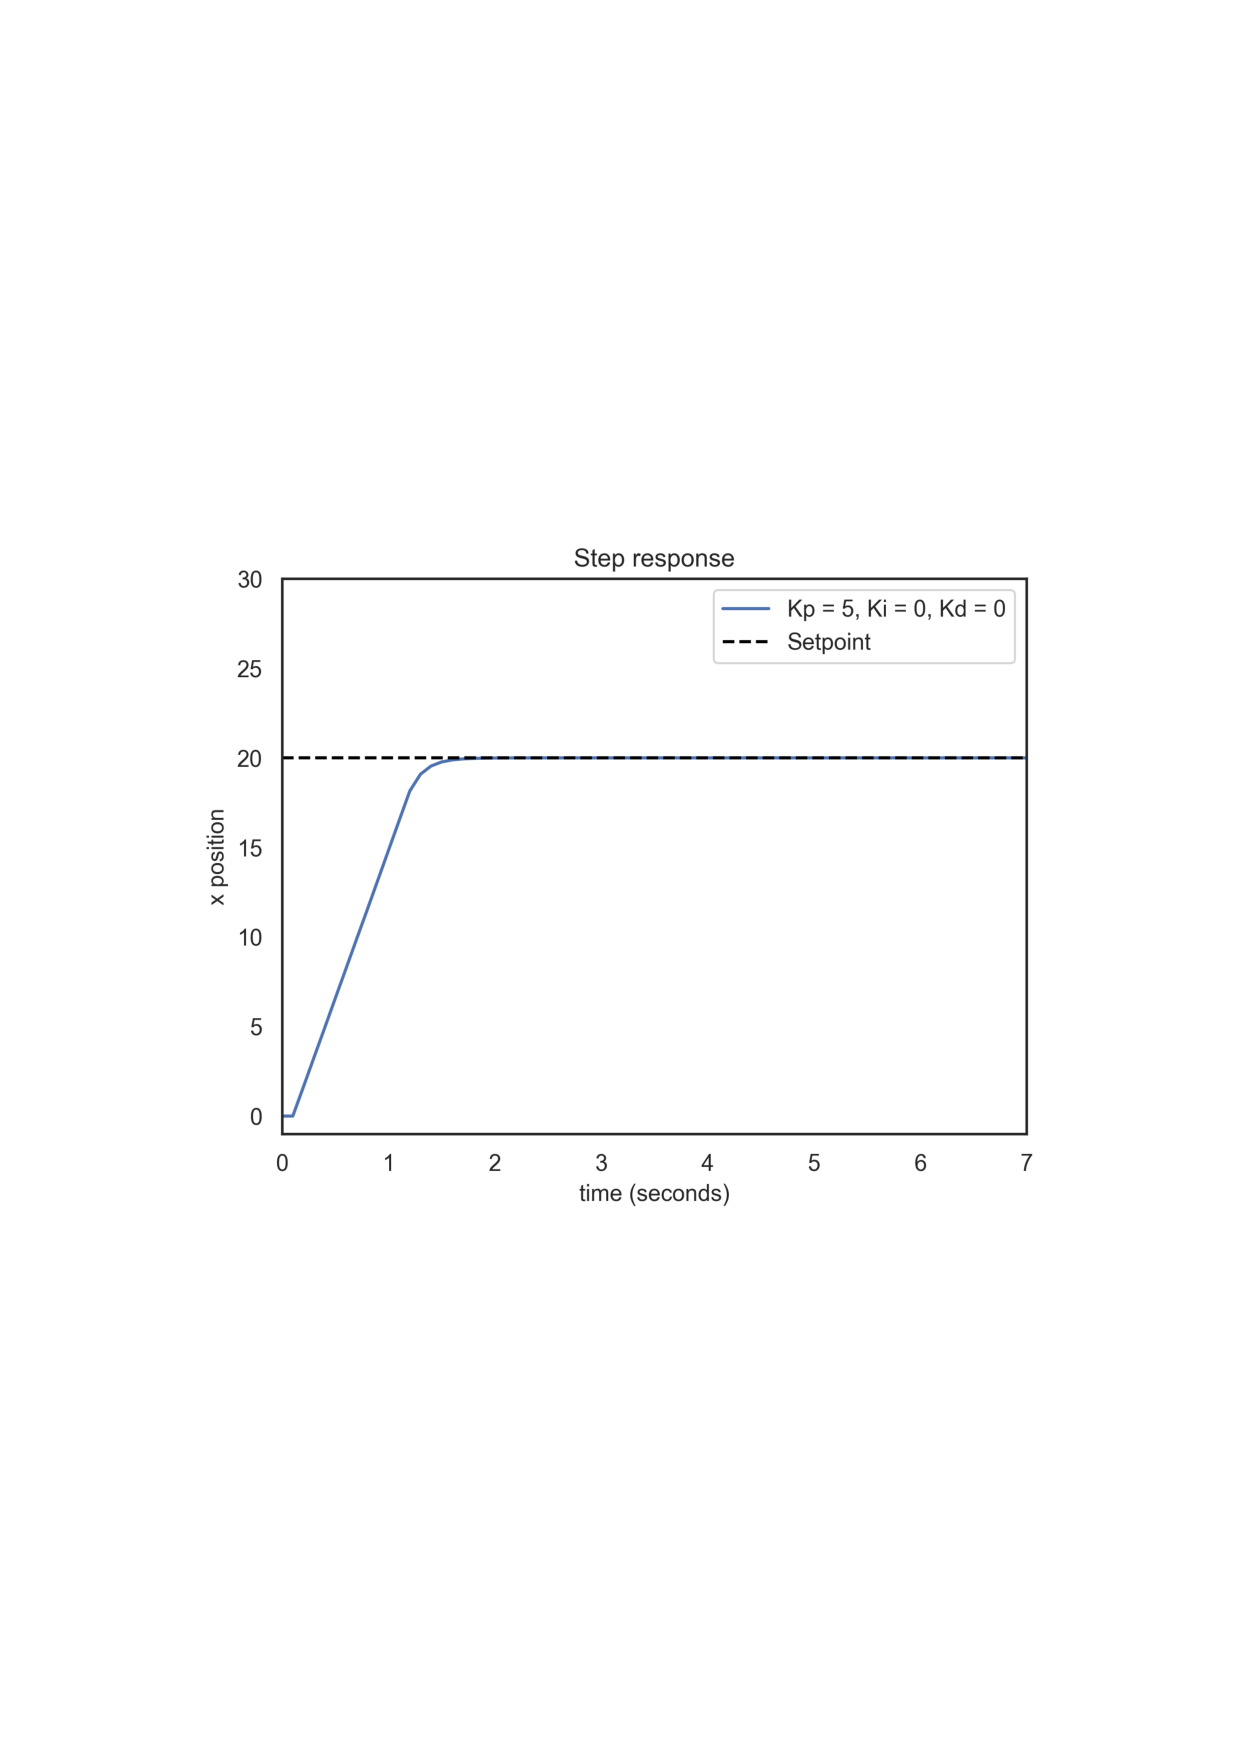
\includegraphics[width=.5\textwidth]{contents/images/Step-responsep=kp5ki0kd0}
	\caption[Step response of the proportinal PID controller.]{Visualisation of the 
		step-response of a P controller with proportional 
		gain $5$.}
	\label{fig:pid}
\end{figure}

It is important to notice that the speed returned by the controller is used to set the 
\texttt{motor\_\{left, right\}\_target}, both with the same value, in order to move 
the robots straight ahead. Moreover, the first and the last robots of the line, 
whose sensors never receive a response respectively from the back and from the 
front, never move.

\subsubsection{Task 2: Colouring the robots in space}
In this scenario, the robots observation, in particular, the sensor readings, do not 
provide useful information about the order of the agents, therefore they are not 
considered to accomplish this task.
On the other hand, if an omniscient controller is not employed, it is impossible to 
solve the problem without using communication, since it is the only way for the 
agents to understand their ordering.

Thus, by initially making all robots transmit the same value, i.e. $0$, we are able 
to establish which are the first and the last robots in the row, or those that do not 
receive any communication respectively from back and front. 
These two agents can at this point start the actual communication by transmitting 
the value they received increased by $1$, that is $1$. 
The following robots will in turn transmit the value they have received increased 
by one. Since the messages received by each of them are two, the agents will in a 
sense, learn to count in order to understand which is the correct value to 
transmit.

The protocol used to decide the communication and the colour, which also 
depends on the amount of robots $N$, or if there are even or odd numbers, is 
shown in Listing \ref{lst:manualtask2}. The colour of each agent in the initial 
configuration is randomly chosen between the two possible colours, red and blue.

\medskip
\begin{python}
	c_left, c_right = get_received_communication(state)
	
	if N % 2 == 1:  # if the number of robots is odd
	
	# Case 1: no communication received from left
	if c_left == 0:
	if c_right > N // 2:
	# the agent is in the first half of the row, so its colour is blue
	message = c_right - 1
	colour = 1
	elif c_right == N // 2:
	# the agent is the central one, so its colour is blue
	message = c_right + 1
	colour = 1
	else:
	# the agent is in the second half of the row, so its colour is red
	message = c_right + 1
	colour = 0
	
	# Case 2: no communication received from right
	elif c_right == 0:
	if c_left > N // 2:
	# the agent is in the second half of the row, so its colour is red
	message = c_left - 1
	colour = 0
	elif c_left == N // 2:
	# the agent is the central one, so its colour is blue
	message = c_left + 1
	colour = 1
	else:
	# the agent is in the first half of the row, so its colour is blue
	message = c_left+ 1
	colour = 1
	
	# Case 3: communication received from both sides
	else:
	if c_left > c_right:
	# the agent is in the second half of the row, so its colour is red
	message = c_right + 1
	colour = 0
	else:
	# the agent is in the first half of the row, so its colour is blue
	message = c_left + 1
	colour = 1
	
	
	elif self.N % 2 == 0:  # if the number of robots is even
	
	# Case 1: no communication received from left
	if c_left == 0:
	if c_right > N // 2:
	# the agent is in the first half of the row, so its colour is blue
	# the situation is ambiguous the message to transmit could be c_right or 
	# even c_right - 1
	message = c_right
	colour = 1
	else:
	# the agent is in the second half of the row, so its colour is red
	message = c_right + 1
	colour = 0
	
	# Case 2: no communication received from right
	elif c_right == 0:
	if c_left < N // 2:
	# the agent is in the first half of the row, so its colour is blue
	message = c_left + 1
	colour = 1
	else:
	# the agent is in the second half of the row, so its colour is red
	# the situation is ambiguous the message to transmit could be c_left or 
	# even c_left - 1
	message = c_left
	colour = 0
	
	# Case 3: communication received from both sides
	else:
	if c_left > c_right:
	# the agent is in the second half of the row, so its colour is red
	message = c_right + 1
	colour = 0
	elif c_left < c_right:
	# the agent is in the first half of the row, so its colour is blue
	message = c_left + 1
	colour = 1
	else:
	# the agent is in the second half of the row, so its colour is red
	message = c_left
	colour = 0
\end{python}

\begin{lstlisting}[frame=none,caption=Protocol used from the manual controller 
to decide for each robot the message to transmit and the colour., 
label=lst:manualtask2]
\end{lstlisting}


\subsection{Learned controller}
\label{subsec:learned}

Usually, to train a network that learns a controller, the states and the actions, 
provided by an expert, need to be observable. For this study, we have decided to 
use instead of the observations of the robots instead of the state, i.e. the positions. 
The reason behind this decision is that in most environments, agents are never 
actually exposed to the full state of the system, instead, they receive partial 
observations, often local or incomplete. In addition, it is frequently too expensive 
to provide the agent with the full state of the system, and sometimes it is not even 
clear how to represent it \cite[][]{ml-agents}.

As the goals to be achieved vary, the controllers should act differently. For this 
reason, we define distinct approaches for the implementation of the controllers 
in the two scenarios.
As regards the first task, we consider two different networks: one distributed that 
act in a supervised way, and one that in addition to predicting the control output 
infers a communication protocol between the agents. 
As concern the second task, we trained one network that predicts the colour 
output and in addition, as before, infers the communication between the robots.

\subsubsection{Task 1: Distributing the robots in space without using 
communication}

Using the data collected through the simulator using the expert controller, it is 
possible to train a very simple ``distributed network'' that takes as input an array 
containing the response values of the sensors – which can be either 
\texttt{prox\_values}, \texttt{prox\_comm} or \texttt{all\_sensors} – and produces 
as output an array containing one float that represents the speed of the wheels, 
which is assumed to be the same both right and left.

The training dataset then contains a fixed number of simulation runs, each 
composed by a variable quantity of time steps. It is important to notice that 
for this approach, unlike the one with communication, it is neither necessary to 
preserve the order of the sequence of time steps, nor to know the exact number 
of agents in the simulation since the network input is the sensing of a single robot.

For this reason, the model is independent of the number of agents and 
consequently it is possible to prove its generalisation capacity, regardless the 
number of robots, by training the networks first on datasets each with a different 
but fixed value of $N$ and then on simulations composed by a variable $N$.
It is easy to show that, although the value of $N$ changes, the network structure 
does not, as it is sufficient during the input preprocessing to change the 
dimension of the input in such a way that all the tensors have the same length, 
fixed at the maximum possible value of $N$, padding those tensors with a lower 
number of agents.

The architecture of the network, displayed in Figure 
\ref{fig:singlenetdistributed1}, is straightforward: there are three linear layers of 
size $\langle\mathtt{input\_size}, 10\rangle$,  $\langle 10, 
10\rangle$ and $\langle 10, 1\rangle$, where \texttt{input\_size} is the 
shape of the sensing that can be either $7$ or $14$.
\begin{figure}[htb]
	\centering
	\begin{subfigure}[h]{0.495\textwidth}
		\centering
		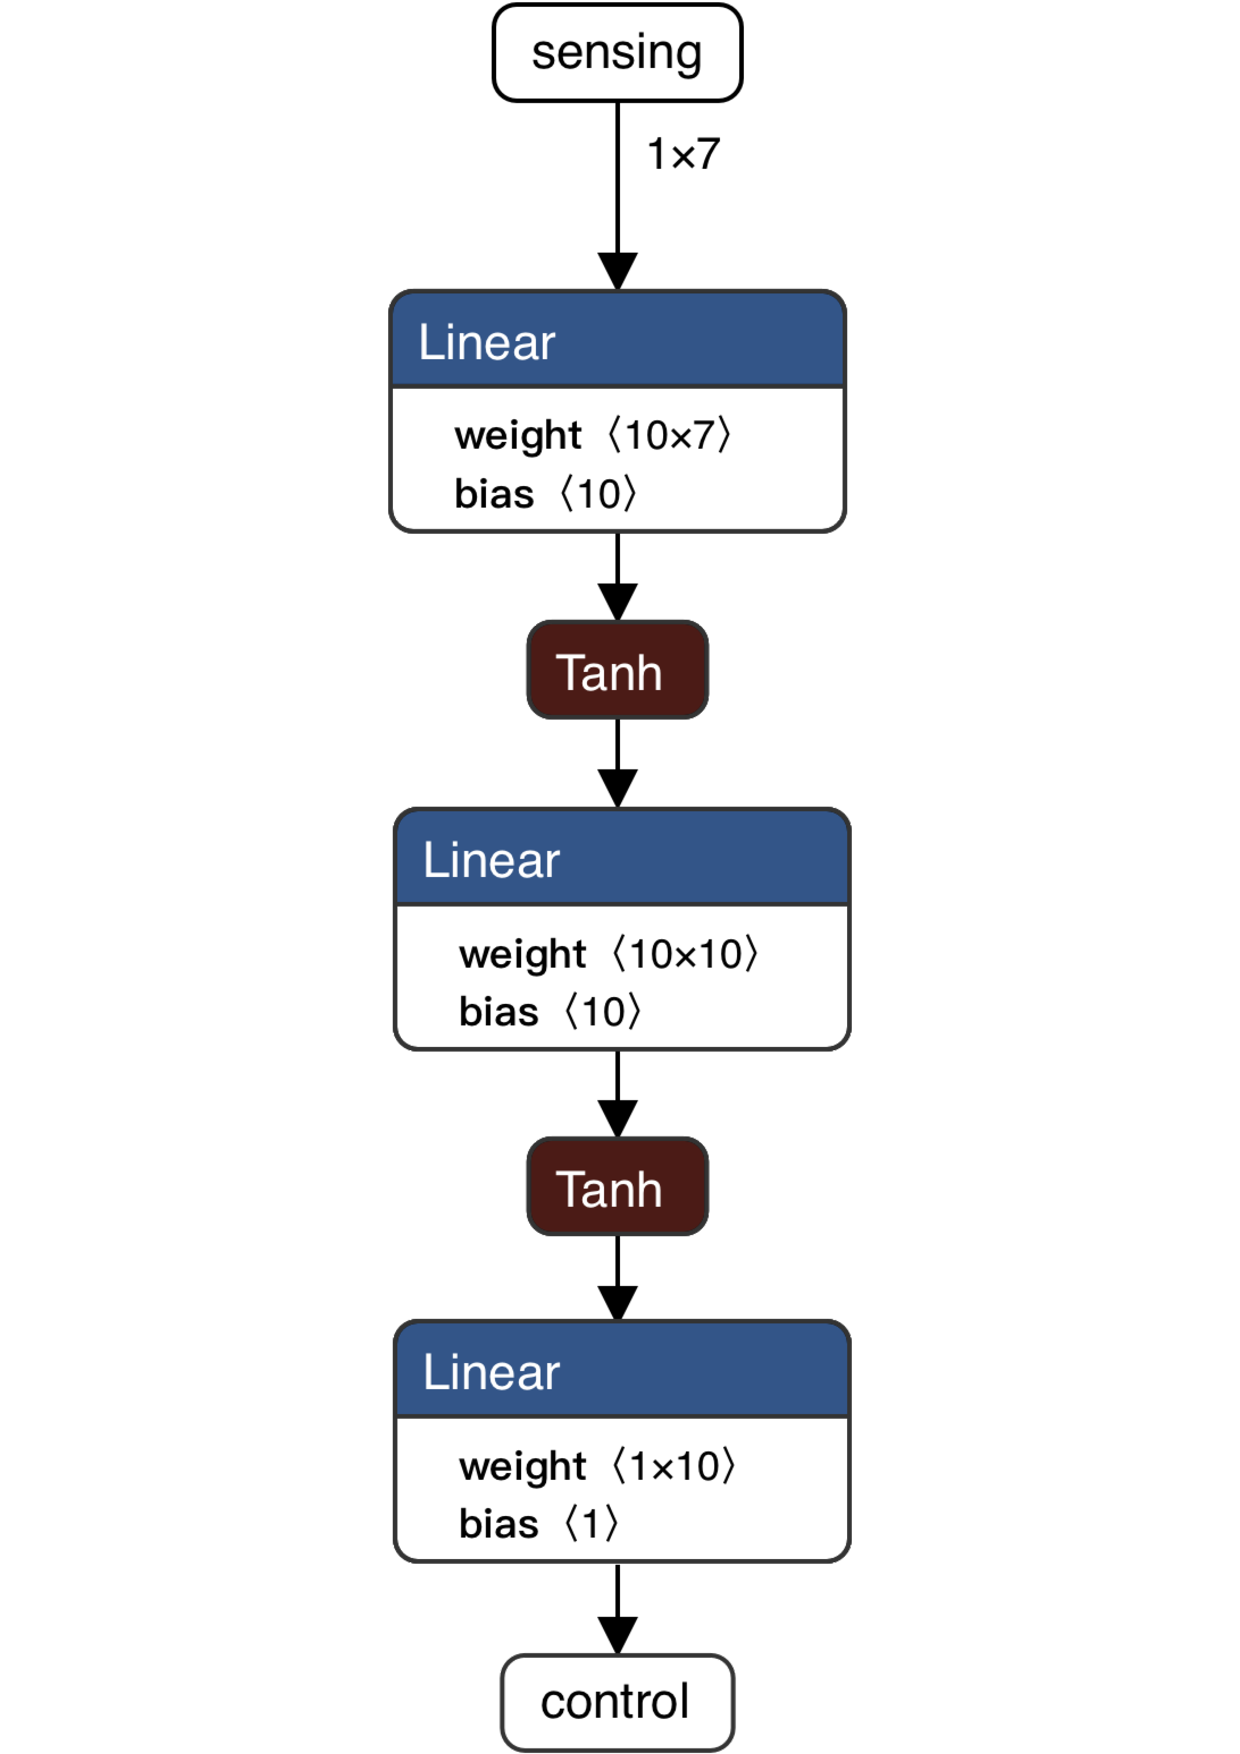
\includegraphics[width=.8\textwidth]{contents/images/task1distributed@4x}%
		\caption{Network with $7$ input sensing.}
		\label{fig:singlenet-d7distributed1}
	\end{subfigure}
	\hfill
	\begin{subfigure}[h]{0.495\textwidth}
		\centering
		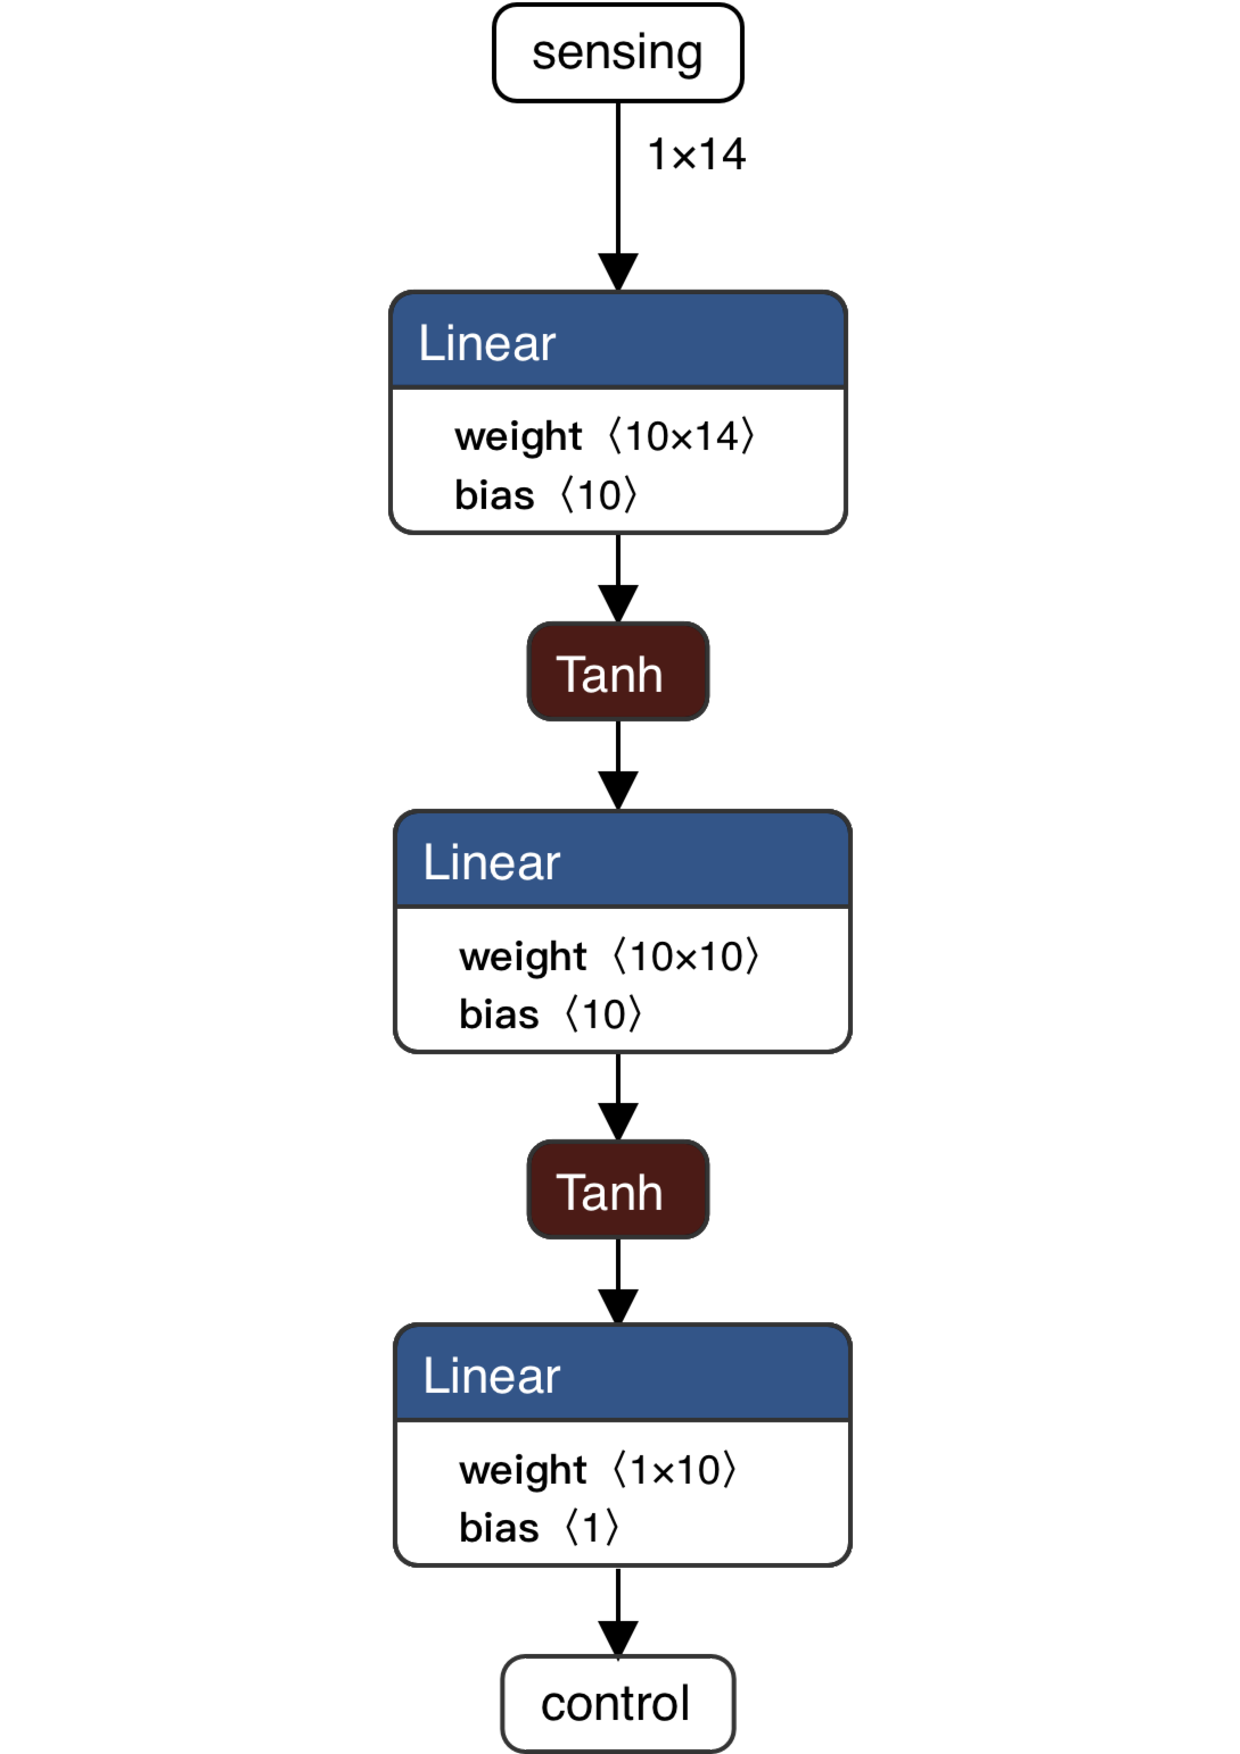
\includegraphics[width=.8\textwidth]{contents/images/task1distributed_all@4x}
		\caption{Network with $14$ input sensing.}
		\label{fig:singlenet-d14distributed1}
	\end{subfigure}
	\caption[Network architectures for the distributed approach.]{Visualisation of 
		the network architecture chosen for the distributed approach.}
	\label{fig:singlenetdistributed1}
\end{figure}

The Tanh non-linear activation function introduced in Section 
\ref{subsec:activationfun}, is applied to the first and second layer. 

As optimiser, we chose Adam, introduced in Section \ref{subsec:optimiser}, 
implemented in the \texttt{torch.optim} package, with a learning rate of $0.01$. 

Instead of performing gradient descent on the entire dataset, the training set is 
split in mini-batches of size $100$ and an approximation of the gradient is 
produced, which makes the algorithm faster and at the same time, for sufficiently 
large batches, the result is indistinguishable.
Gradient descent algorithms are susceptible to ``get stuck'' in local minima.
Mini-batches shuffle facilitate to avoid this problem by enabling the gradient to 
``bounce'' out of eventual local minimum, making it more variable by exploiting 
randomness, thereby helping convergence \cite[][]{meng2019convergence}.

All the models are trained for $50$ epochs and evaluated using the \gls{mse} loss 
function, defined in Section \ref{subsec:lossfunctions}, implemented in the 
\texttt{torch.nn} package.

\subsubsection{Task 1: Distributing the robots in space using communication}
\label{subsubsec:task1comm}

An alternative to the previous approach involves training a distributed network 
that also exploits a communication protocol between agents to decide more 
reliably the output control. 
Thus, using the same data collected before, we build a model that at each time 
step takes as input an array containing the response values of the sensors for each 
robot – \texttt{prox\_values}, \texttt{prox\_comm} or \texttt{all\_sensors} – and 
the messages received in the previous time step, communicated by the nearest 
agents (on the left and on the right), and produces as output 2 floats: the control, 
which, as before, is the speed of the wheels, and the communication, i.e. the 
message transmitted by the robot to the two nearest agents.

Even for this purpose, the model is independent of the number of agents in 
the simulations. Instead, now it is important to keep track of the time steps order 
since the input of the network requires the communication received which 
corresponds to the messages transmitted in the previous time step. To do so, a 
preprocessing is applied to the dataset to combine consecutive 
time steps into a set of sequences. Therefore, we divide each simulation in 
sequences of length $2$, composed of two successive observations for each 
robot, using a stride of $1$.   
Accordingly, the shape of the model input has been transformed from $1 \times 
\mathtt{input\_size}$ to $\mathtt{seq\_length} \times \mathtt{N} \times 
\mathtt{input\_size}$, where \texttt{seq\_length} is fixed at $2$, $N$ is variable 
and \texttt{input\_size} can be $7$ or $14$.

\begin{figure}[!htb]
	\centering
	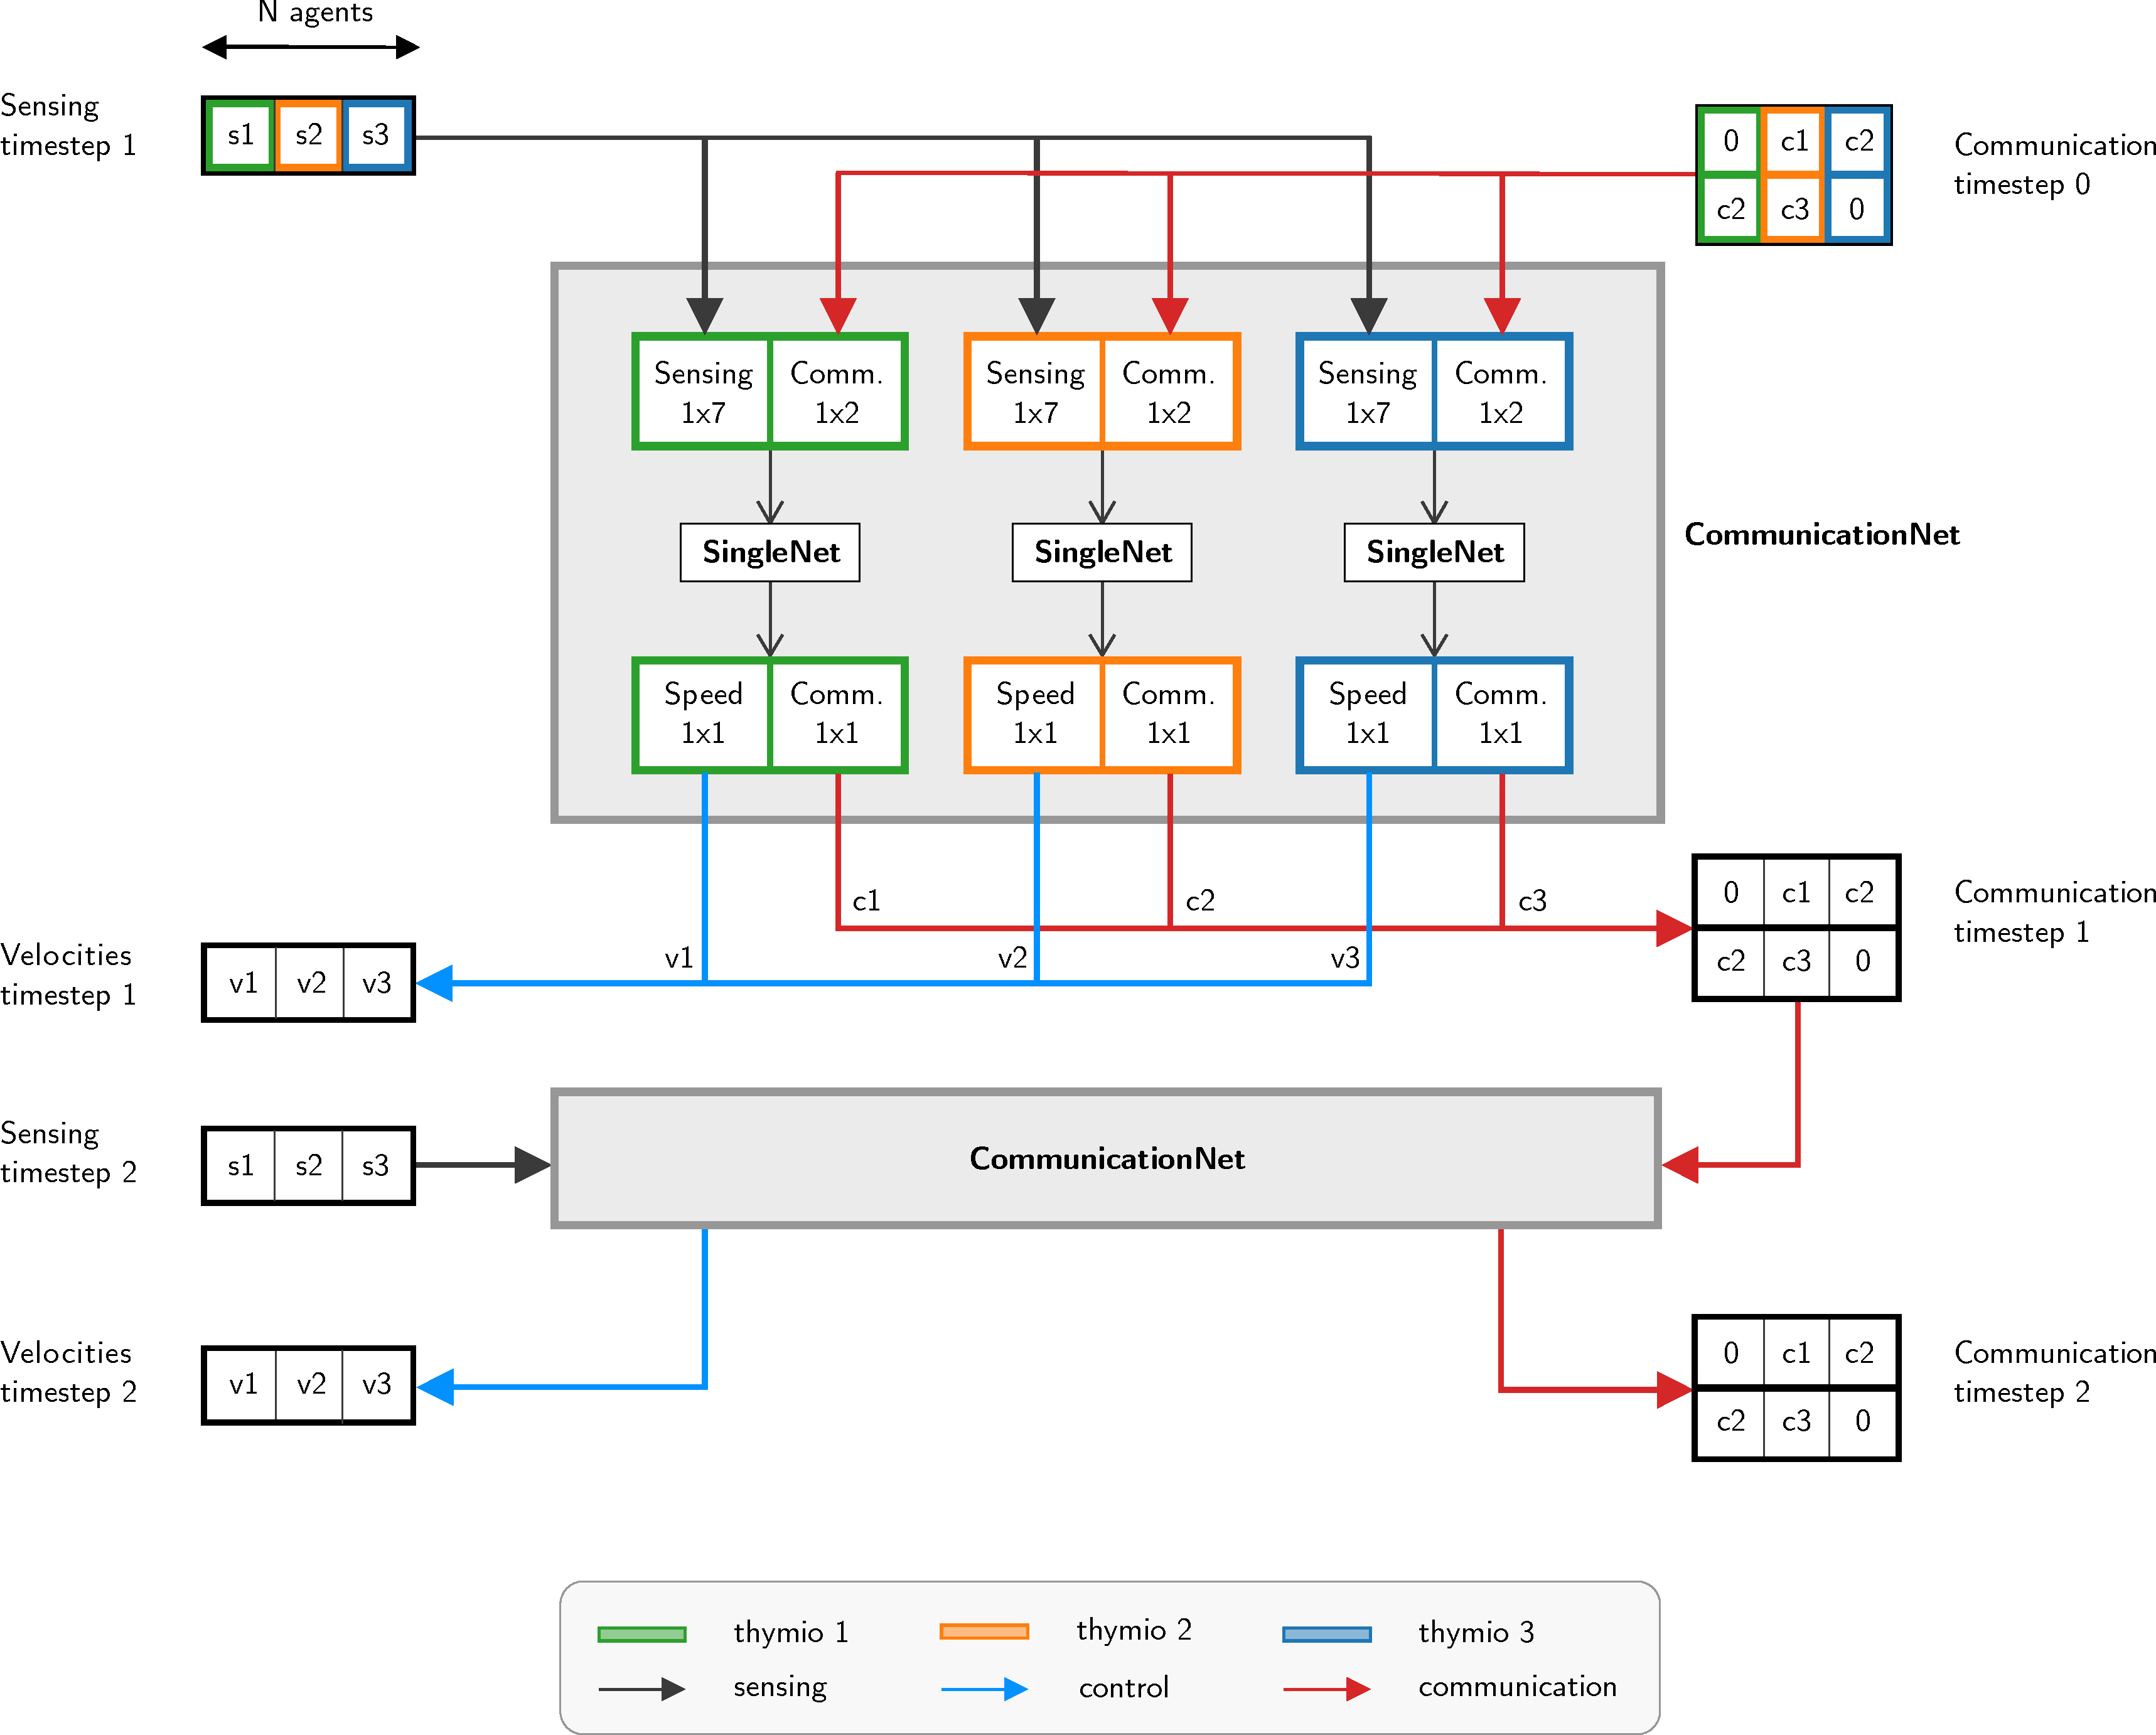
\includegraphics[width=\textwidth]{contents/images/commnet2}
	\caption[Communication network.]{Visualisation of the forward pass of the 
		communication network with three agents and a sequence composed by two 
		time steps.}
	\label{fig:commnet1}
\end{figure}

It is important to notice that the communication is not yet in the input since 
it is not contained in the original dataset, instead is treated as a hidden 
variable to be inferred. 
At the beginning of each sequence, there are no previous time steps to consider 
since no messages have been received yet. Therefore, a placeholder is randomly 
initialised, filled with float values in the range $[0, 1]$. 
The size of this array corresponds to the number of agents plus two elements, one 
at the beginning and one at the end of the vector, always set to $0$ since they are 
used to store the fact that the two extreme robots never receive messages 
respectively from the left or from the right. 
The random initialisation of this vector is essential to increase the generalization 
capabilities of the network during its training, showing it different starting 
situations.
Therefore, this corresponds to a static unroll of a \gls{rnn}.%FIXME \cite[][]{}.

As a consequence, we define a recurrent structure of the communication 
network, shown in Figure \ref{fig:commnet1}.
It is composed by two nested modules: in the outer level operates the 
\texttt{CommNet} that handles the sensing of all the agents, while in the inner the 
\texttt{SingleNet} that works on the sensing and the communication received by a 
single agent in a certain time step, producing as output the control and the 
communication to transmit. 

The architecture of the \texttt{SingleNet}, displayed in Figure 
\ref{fig:singlenetcomm1}, is almost the same as the one of the distributed 
model without communication: there are three linear layers each of size 
$\langle\mathtt{input\_size}, 10\rangle$,  $\langle 10, 10\rangle$ and $\langle 
10, 2\rangle$, where \texttt{input\_size} is the sum of the shape of the sensing 
and the two communication values received, one from the left and one from the 
right.

\begin{figure}[!htb]
	\centering
	\begin{subfigure}[h]{0.495\textwidth}
		\centering
		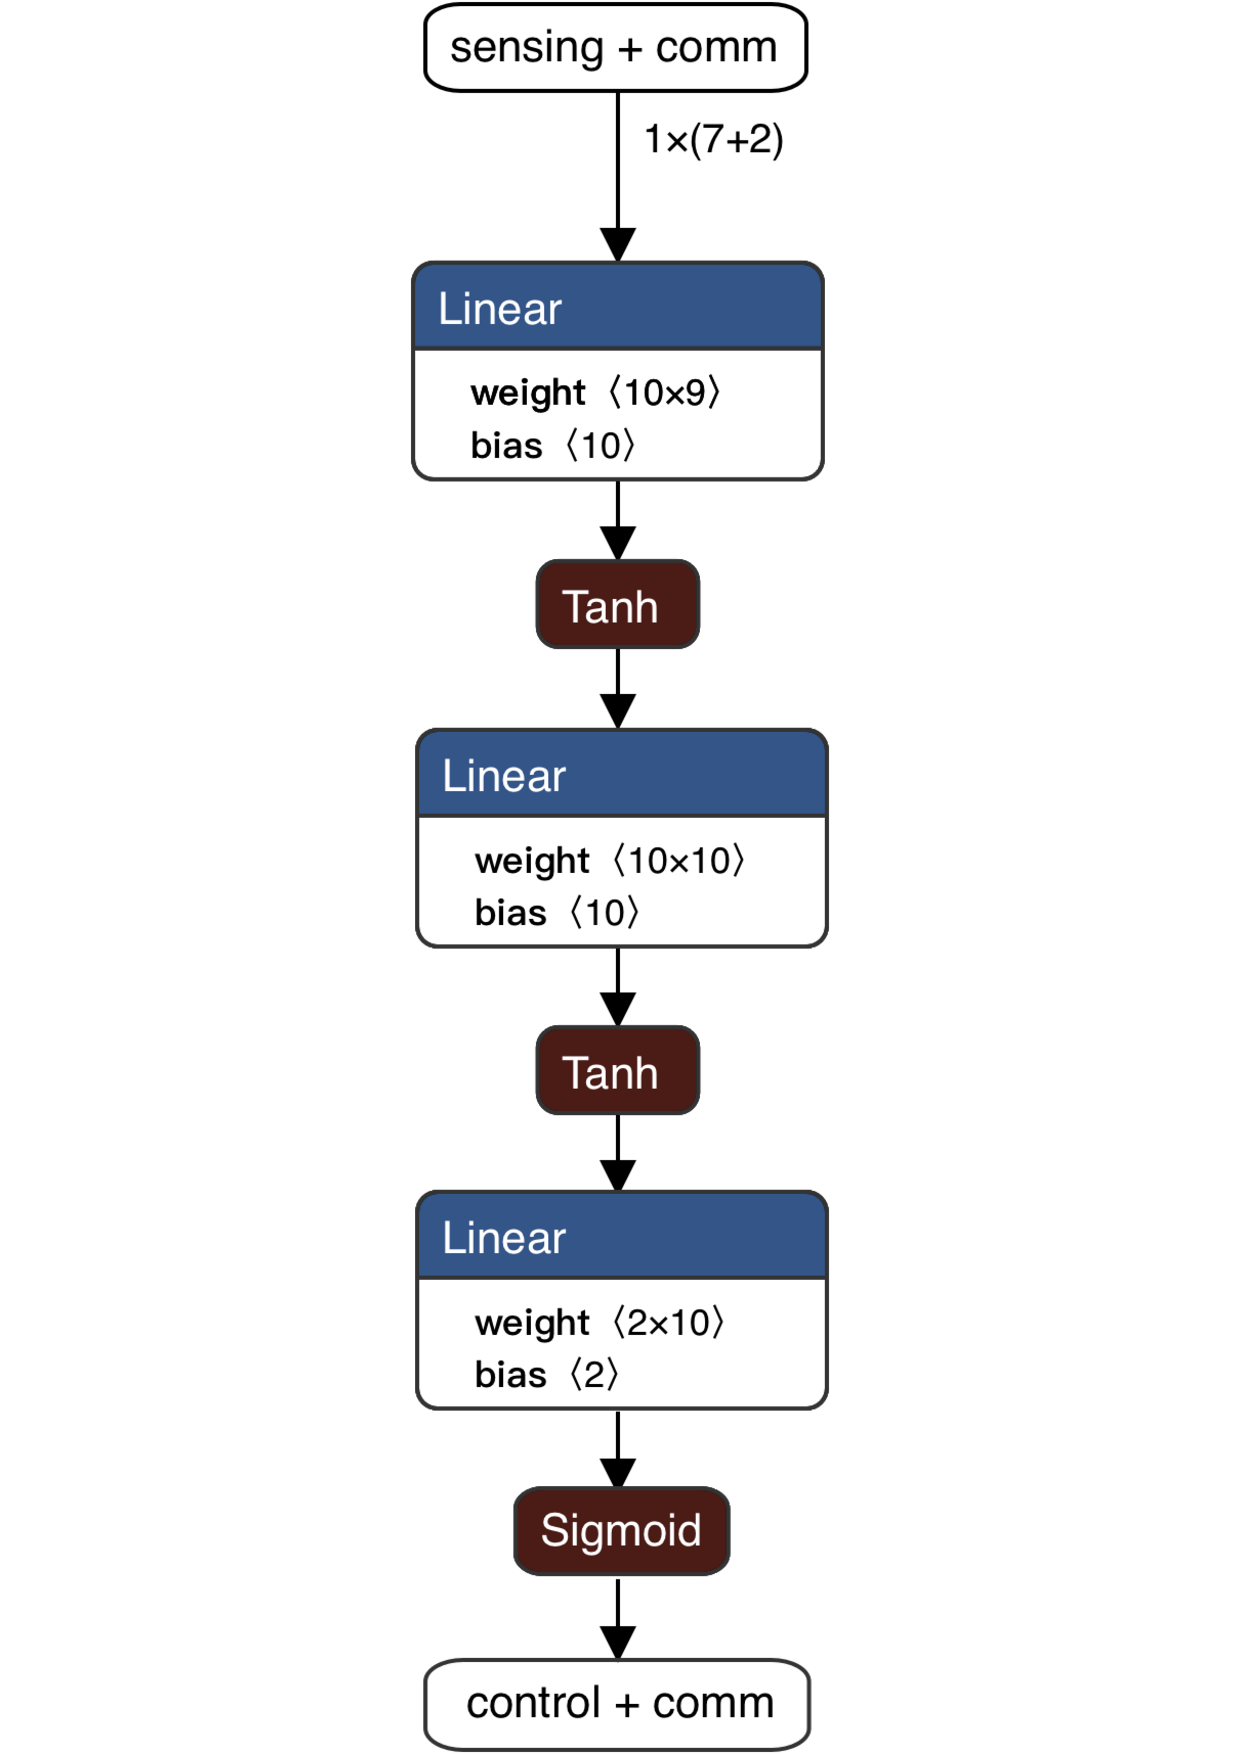
\includegraphics[width=.8\textwidth]{contents/images/task1distributedcomm@4x}%
		\caption{\texttt{SingleNet} with $7$ input sensing.}
	\end{subfigure}
	\hfill
	\begin{subfigure}[h]{0.495\textwidth}
		\centering
		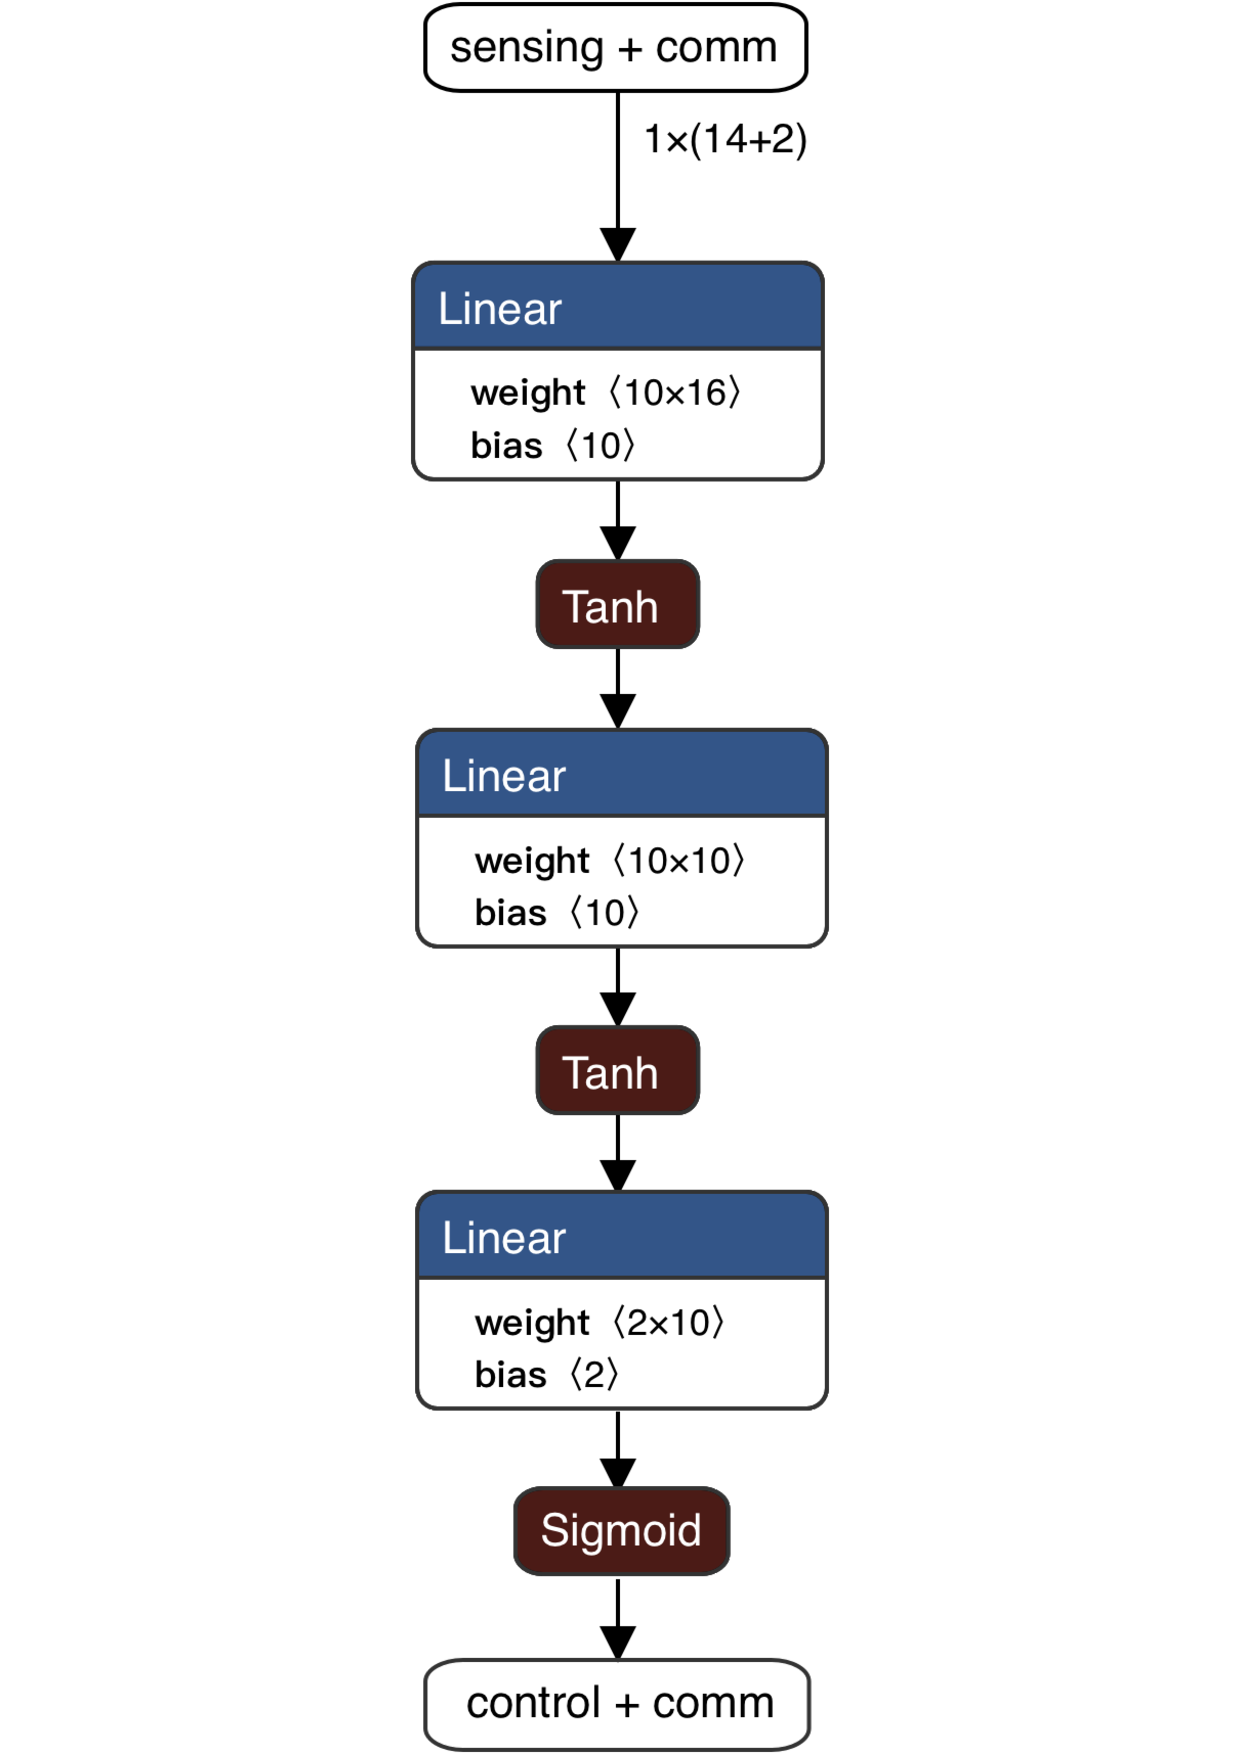
\includegraphics[width=.8\textwidth]{contents/images/task1distributed_allcomm@4x}
		\caption{\texttt{SingleNet} with $14$ input sensing.}
	\end{subfigure}
	\caption[Network architectures for the distributed approach with 
	communication.]{Visualisation of the network architecture chosen for the 
		distributed approach with communication in case of 7 or 14 inputs.}
	\label{fig:singlenetcomm1}
\end{figure}

As before, a Tanh non-linear activation function is applied to the first and second 
layer, while a sigmoid, introduced in Section \ref{subsec:activationfun}, is applied 
to the second dimension of the output in order to normalise it in the range $[0, 
1]$.

As before, we use Adam optimiser, addressed in Section \ref{subsec:optimiser}, 
but with a smaller learning rate, $0.001$. 
We split the dataset in mini-batches, this time of size $10$ and then we train 
the models for $500$ epochs. 
Finally, we evaluate the goodness of the predicted control using the \gls{mse} 
loss function, while the communication is learned in an unsupervised way.
Since the network is fully connected, the communication affects directly the 
output, and consequently, the error minimised, even if it is computed using 
only the control. Improving the loss has an impact also on the communication 
latent variable: since the error is propagated through the internal network, in 
order to update the weight during the back-propagation step, that influences the 
communication.

\subsubsection{Task 2: Colouring the robots in space}
In this scenario, it is possible to implement a network very similar to that used for 
the previous task, that is the distributed approach with communication, described 
in Paragraph \ref{subsubsec:task1comm}, but this time ignoring the sensors 
readings.
Thus, using the same data collected before we build a model that at each time 
step takes as input for each robot only the message received in the previous time 
step, communicated by the nearest agents (on the left and on the right), and 
produces as output an array of 2 floats, the first one is the probability of the agent 
top \gls{led} to be blue and the second is the communication, i.e. the message to 
be transmitted by the robot.

The communication network, which structure is shown in Figure 
\ref{fig:commnet2}, is composed by two nested modules: in the outer-level 
operates the \texttt{CommNet} that handle the sensing of all the agents, while in 
the inner-level the \texttt{SingleNet} that works on the communication received 
by a single agent in a certain time step, producing as output the colour and the 
communication to transmit. 
\begin{figure}[H]
	\centering
	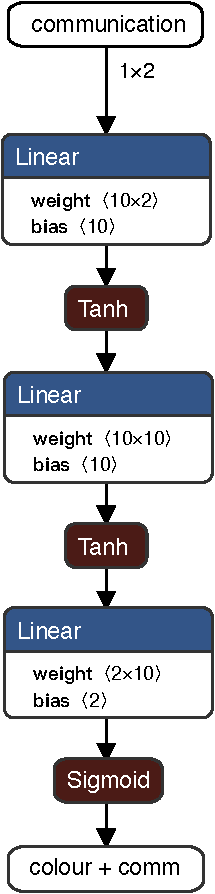
\includegraphics[width=.14\textwidth]{contents/images/task2allcomm}
	\caption[Network architectures for the communication approach.]{Visualisation 
		of the network architecture chosen for the 
		communication approach.}
	\label{fig:singlenetcomm2}
\end{figure}

The \texttt{SingleNet}, displayed in Figure \ref{fig:singlenetcomm2}, is composed 
by three linear layers of size $\langle \mathtt{input\_size}, 10\rangle$,  $\langle 
10, 10\rangle$ and $\langle 10, 2\rangle$, where \texttt{input\_size} 
corresponds to the two communication values received, one from the left and one 
from the right.


\begin{figure}[!htb]
	\centering
	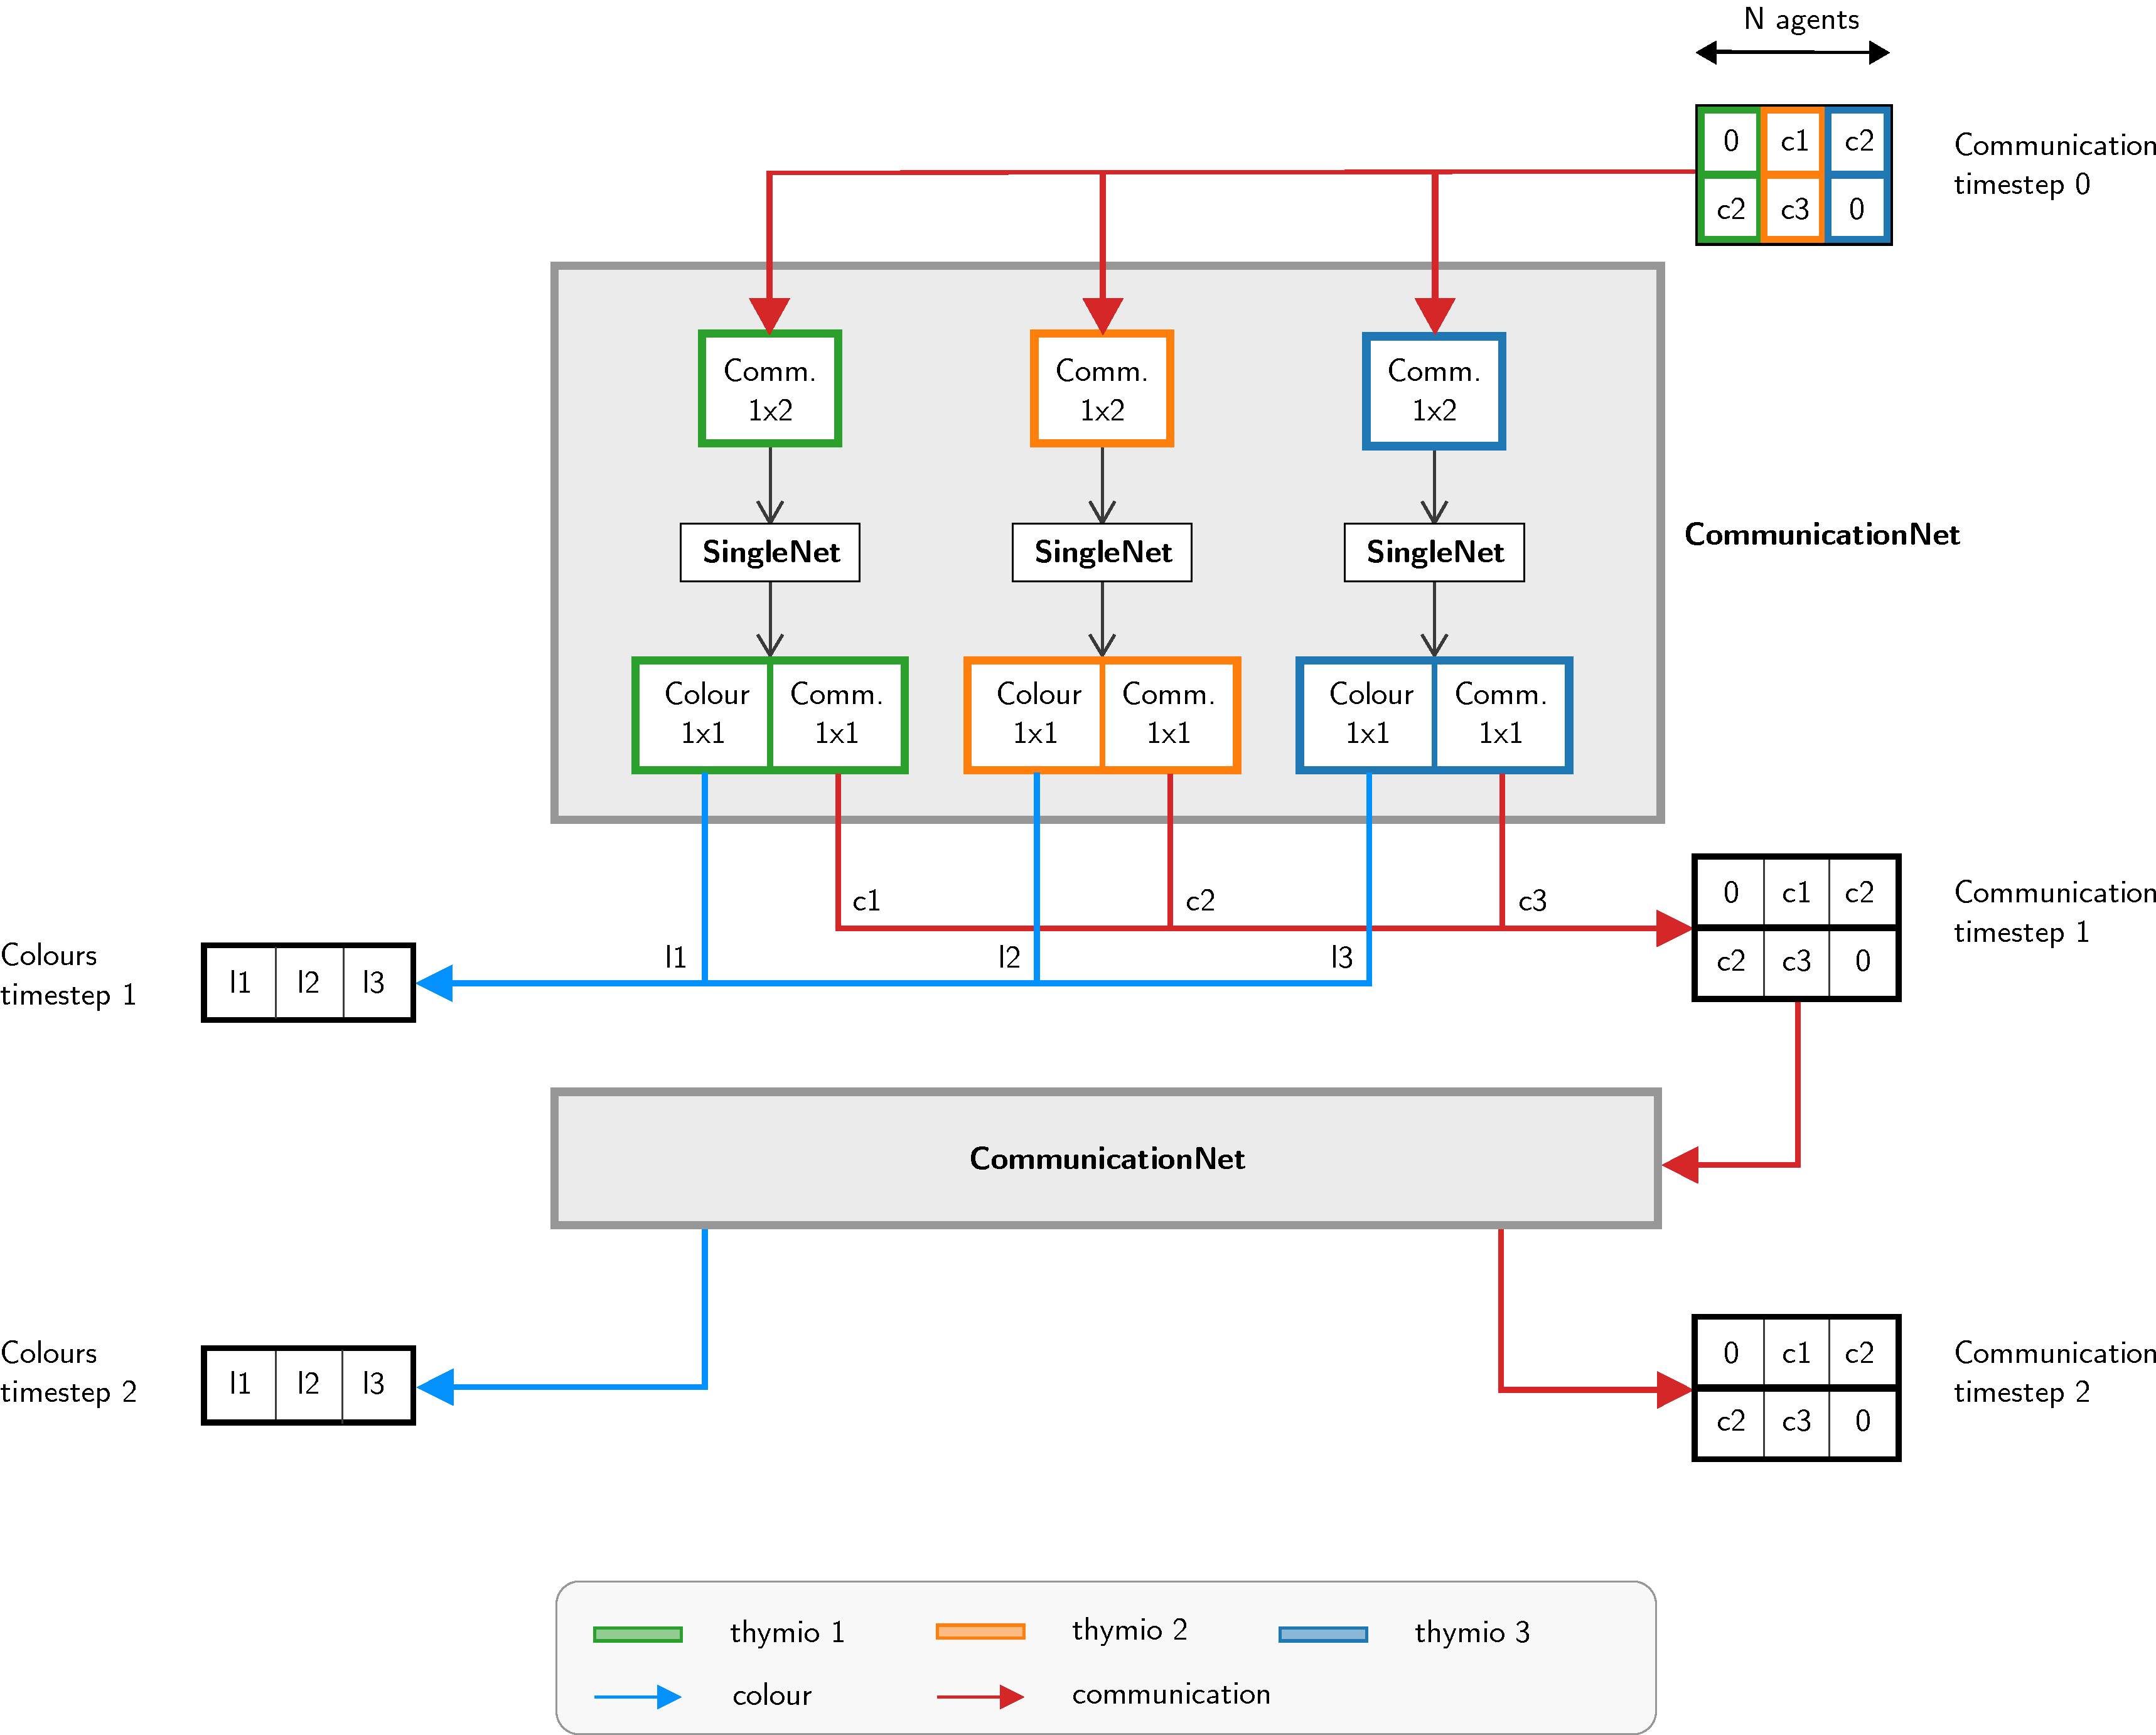
\includegraphics[width=\textwidth]{contents/images/commnettask2}
	\caption[Communication network of the second task.]{Visualisation of the 
		forward pass of the communication network with three agents and a 
		sequence 
		composed by two time steps.}
	\label{fig:commnet2}
\end{figure}

The activation functions used for this purpose are two,  the \emph{hyperbolic 
tangent} (Tanh) and the \emph{sigmoid}, introduced in Section 
\ref{subsec:activationfun}.
To the first and second layer is applied a Tanh non-linear activation function, 
while a sigmoid to the output, in order to normalise it in the range $[0, 1]$.


As before, we use Adam optimiser but with a smaller learning rate, $0.001$. 
We split the dataset in mini-batches of size $10$ and then we train the models for 
$100$ epochs. 

In order to decide the metric to evaluate the goodness of the prediction, it is 
necessary to analyse the output of the network. As we said, the model returns, in 
addition to the communication, the colour that is actually the probability of the 
agent top \gls{led} to be blue. This means that, when the network produces a 0, 
the probability that the \gls{led} is blue is equal to 0, i.e. is red, in the same way, 1 
means that instead, this will be blue. In this way, we define a simple policy 
function that returns the colour blue when the probability is between 0.5 and 1, 
and red otherwise, or when the probability is less than 0.5.
For this reason, instead of using the \gls{mse} loss function, as this is a binary 
classification problem we choose the \gls{bce}, defined in Section 
\ref{subsec:lossfunctions}, implemented in the \texttt{torch.nn} package.
It is important to remember that communication is still learned in an unsupervised 
way.


\chapter{Implementation and tools}
\label{chap:impl}

\section{Thymio II}
\label{sec:thymio}

The target platform chosen is Thymio II, a small differential drive mobile robot 
developed in the context of a collaboration between the MOBOTS group of the 
\gls{epfl} and the \gls{ecal}. 

Thymio runs the Aseba open-source programming environment 
\cite[see][]{magnenat2010aseba}, an event-based modular architecture for 
distributed control of mobile robots, designed to enable beginners to program 
easily and efficiently \cite[][]{mondada2017bringing}, making it well-suited for 
robotic education and research.

Another particularity of this tool is the integration with the open-source 
\gls{ros} \cite[][]{quigley2009ros}, through asebaros bridge \cite[][]{asebaros}. 

The Thymio II includes sensors that can measure light, sound and distance. It can 
perform actions such as move using two wheels, each powered by its own motor, 
but also turning lights on and off.

\subsection{Motors}
\label{subsection: motors}
The robot is equipped with two motors, each connected to one of the two 
wheels, which allow the robot to move forward, backward but also turn by setting 
the velocity of the wheels at different speeds. The maximum speed allowed to the 
agent is $16.6$ \gls{cm/s}.

\chapter{Experiments and results}
\label{chap:experiments}

%\section{Overview}
%\label{sec:overview}

In this work, we investigate collaborative multi-agent problems in a \gls{1d} 
simulated environment.

The environment is represented by a Cartesian plane, a system of coordinates
defined by two perpendicular axes, $x$ and $y$. 

In this scenario, $N$ robots, all oriented in the same direction, are initially 
randomly placed along the x-axis, avoiding collisions and in such a way the 
average gap among the agents is included in the proximity sensors' ranges. 
All the robots act in collaboration to achieve a common goal, however the first 
and last in the row behave like walls. %% FIXME

The agent is a point on the plane, formally described by a homogeneous vector 
with respect to the world coordinate frame $W$, obtained multiplying the 
homogeneous vector of the point, with respect to the robot coordinate frame 
$A$, by a homogeneous transformation. 

The relative pose $A$ of each agent is identified by a $3 \times 3$ matrix 
$\mathbf{T}$, with respect to the world reference frame $W$. 

\begin{Equation}[!htb]
	\centering
	\begin{equation}
	{^W\!\xi_A} = {^W\!\mathbf{T}_A} 
	=
	\begin{pmatrix}
	^W\!\mathbf{R}_A & ^W\!\mathbf{t}_A\\
	0, 0 & 1
	\end{pmatrix}
	=
	\begin{pmatrix}
	\cos \theta & - \sin \theta & t_x\\
	\sin \theta & \cos \theta & t_y\\
	0 & 0 & 1
	\end{pmatrix}
	\end{equation}
	\caption[Homogeneous transformation matrix.]{The homogeneous 
	transformation matrix, 	$^W\!\mathbf{T}_A$, includes $^W\!\mathbf{R}_A$, a 
	$2 \times 2$ rotation matrix and $^W\!\mathbf{t}_A$, a $2 \times 1$ 
	translation vector.}
	\label{eq:hommatrix}
\end{Equation}

However, since we are in a \gls{1d} environment, the $y$ coordinate is equal 
to $0$ and also the orientation angle $\theta$ must be zero as all the agents are 
oriented as the world frame. 

Moreover, we can consider the agents as holonomic, since their movements are 
limited in only one dimension. This premise simplifies our system, in which 
consequently we have to keep into account only geometric constraints and not
kinematic.

\section{Assumptions}
\label{sec:assum}
%%FIXME synonim
Before diving in a detailed explanation of the experiments, it is necessary to 
formulate some assumptions.

Of fundamental importance is the approach adopted for the generation of the 
initial positions of the robots.
The initial configurations need to be randomly generated, verifying that there is 
no bias towards those close to the target.
In particular, once established the number of agents to spawn and the average 
gap between them, a vector containing samples, each representing a real random 
gap, is drawn from a uniform distribution in the interval $[0, 
2*\mathtt{avg\_gap})$. 
At each gap is adde the value that corresponds to the length of the Thymio, that is 
$10.9$ \gls{cm}, and finally, the final positions are obtained return the cumulative 
sum of the elements in the generated vector. 

Another premise regards the sensors of the Thymio. 
As introduced in Section \ref{subsec:enkisensors}, we have available 
\texttt{prox\_values} and \texttt{prox\_comm\_events.intensities}. In order to be 
used, the \texttt{prox\_comm\_events.intensities} should be flatten in order to 
obtain a single array enclosing the intensities recorded by the possible events. 
To do so, we decided to create a new array, called \texttt{prox\_comm}, by 
keeping for each element of it only the value that has the maximum intensity 
chose among all the possible values in the corresponding position, (in our case 
maximum $2$).
In addition, we define another variable, name \texttt{all\_sensors}, that is an array 
of $14$ intensities result of the combination of the \texttt{prox\_values} and 
\texttt{prox\_comm} vectors.

\section{Controllers}
\label{sec:controllers}

In a \gls{mas}, each agent can perceive the environment through sensors 
acquiring a total or partial knowledge of it. The observations extracted can be 
used by a controller, together with the current state of the agent, to determine 
actions, draw inferences and finally solve tasks. 

In an imitation learning setting, there are two controllers involved: an expert 
controller, which performs the desired task with perfect knowledge of the 
environment, and a learned controller, which is trained to imitate the behaviour 
of the omniscient controller.

For each of the task that we are going to face, we introduce three controllers: the 
expert controller, that exploits its complete knowledge of the state of the system 
to decide the best action to perform, the manual controller, that has only a partial 
knowledge of it, and a controller learned by imitating the expert one.

These controllers will be described in detail later in the sections dedicated to each 
task.

\section{Datasets generation}
\label{sec:dataset}

Relying on the simulator Enki, introduced in Section \ref{sec:enki}, two datasets 
containing $1000$ simulation runs each, are generated for the omniscient and 
the manual controllers. 

Each run, that differs from the others for the initial positions where are spawn the 
agents, sets up a world containing $N$ Thymio. 
In particular, for all the simulations are chosen randomly the number of agents 
$N$, within the range $[5, 10]$, and the \texttt{avg\_gap}, that is the average 
distance among the robot in the final configuration of the run, that can be in the 
range $[5, 24]$.
%, which means that the robots can sense each other using \texttt{prox\_values} 
%and \texttt{prox\_comm} together.

A simulation run is stopped either immediately after all the robots reach the 
target pose, with a certain tolerance, or after $4$ \gls{s} ($40$ timesteps).

At each timestep, all the useful information regarding the agents are stored in the 
dataset, such as the index of the timestep, the sensor readings, the pose of the 
robot, the motors target, the communication transmitted and received and finally 
its colour.

The dataset generated using the expert controller is the one used to train the 
models, while the one generated with the manual controller is used as a baseline 
for the comparison with the learned model.

Through the experiments we trained different models varying the input of the 
network, that can be \texttt{prox\_values}, \texttt{prox\_comm} or 
\texttt{all\_sensors}, the number of agents and the average gap distance between 
them, that can both be fixed to a certain value or being variable.

\section{Task 1}
\label{sec:task1}

\subsection{Overview}
\label{subsec:desc1}

The first scenario tackles an interesting multi-agent coordination task, the 
distribution of robots in space.

As described in the overview of Chapter \ref{chap:experiments}, which provides 
additional details, are spawned in a ``single file'' N robots at random positions.
Each agent can update its state – its absolute position – by performing actions – 
moving forward and backwards along the x-axis – based on the observations 
received from the environment – the distances from neighbours – using its 
sensors. They are also able to transmit and receive a communication value to 
peer robots within a range of about $48$\gls{cm}. 
A full explanation of how communication works for Thymio II is covered in 
Section \ref{subsec:thymiocomm}.

As a consequence of the \gls{1d} environment, the agents' movements are 
limited to two directions: moving forward along the x-axis when the velocity is 
positive, while going backwards when it is negative. 

The robots share a common goal: arrange themselves uniformly along the 
line between the two ``dead'' robots, in such a way they stand at equal distances 
from each other.

This problem represents a cooperative goal that can be reached by performing 
imitation learning, that means training an end-to-end \gls{nn} by following 
the example of an omniscient controller, introduced in Section 
\ref{subsubsec:omniscient}.
Exploiting its complete knowledge of the environment, the expert is able to 
decide the best action to perform.

In the course of this study, we tried to understand if it is possible to use a 
controller learned by imitation, instead of using a manual one. In particular, we 
focus on two approaches, presented in Sections \ref{subsec:dist} and 
\ref{subsec:comm}.
In both cases, we train \glspl{dnn} that receive sensor inputs and produce 
commands for the motors, but for the second alternative, the network has an 
addition input – the received communication transmitted by the neighbouring 
agents in the previous timestep – and an extra output – the message to be sent.

\subsection{Controllers}
\label{subsec:task1controllers}

\subsubsection{Expert controller}
\label{subsubsec:omniscient}

As disclosed in Section \ref{subsec:controllersmodel}, the first element involved in 
an imitation learning problem is the omniscient controller, also called expert.

This controller perceives the environment and the observations of all the agents, 
obtaining a global knowledge of the state of the system. In this way it can use all 
the information that it owns to decide the best action to perform for all the 
agents. 

In this first scenario, the omniscient controller, based on the current poses of the 
robots, moves the agents at a certain speed to reach the target positions. In 
particular, the linear velocity of each agent is computed as a ``signed distance`` 
between the current and the goal position of the robot, along its theta. 

Formally, given the current pose, defined by the triple $(x, y, \theta)$ and the 
target pose $(\overline x, \overline y, \overline \theta)$, the signed distance $d$ 
is computed as follow:
\begin{Equation}[!htb]
	\centering
	\begin{equation}
	d = \left(\overline x * \cos (\theta) + \overline y * \sin (\theta)\right) -
	\left( x * \cos (\theta) + y * \sin (\theta)\right)
	\end{equation}
	\caption[Signed distance function.]{Function used to compute the ``signed 
	distance'' between the current and the goal position of a robot.}
	\label{eq:signeddist}
\end{Equation}

\noindent
To obtain the final velocity of the agent, this quantity is multiplied by a constant, 
we choose $10$ to keep the controller as fast as possible, and then clipped to its 
maximum value, $16.6$\gls{cm/s}.

This controller can be informally considered as a simple Bang Bang controller 
since the optimal controller moves the robot at maximum speed towards the 
target unless the target is closer than \texttt{control\_step\_duration} $\times$ 
\texttt{maximum\_speed}. In this case, the agent is moved slower then the 
maximum allowed speed so that at the end of the timestep it is located exactly at 
the target.

Unfortunately, using an omniscient controller to solve this kind of problems is not 
realistic nor feasible in a real environment.

\subsubsection{Manual controller}
\label{subsubsec:manual}
The second controller we want to discuss/write about is the manual one, whose 
main purpose is to draw conclusions about the quality of the controller learned.

The main difference between this and the previous controller is that, the manual 
one can be considered a local distributed controller, that only has a partial 
knowledge of the environment since knows only the state of the current agent 
and its observations.

This controller moves the robots towards the target by minimising the difference 
between the values recorded by the front and rear sensors, trying to maintain the 
maximum achievable speed.

For each agent the controller is the same and, if given an identical set of 
observations as input, likewise, the outputs will be equivalent.

The one implemented is a proportional controller, a particular variant of \gls{pid}
with only the $K_p$ term. 
The closed-loop control uses a feedback to adjust the control while the action 
takes place in proportion to the existing error. This function, given a desired 
output $x(t)$, or set point, produces an output $y(t)$, or process variable, such 
that the error $e(t)$ is obtained as the difference between the value of the set 
point and the process variable. Finally, the control variable $u(t)$ is the output of 
the \gls{pid} controller and is computed as follows:

\begin{Equation}[!h]
	\centering
	\begin{equation}
	u(t) = K_p * e(t)
	\end{equation}
	\caption[Proportioal PID controller.]{Proportional \gls{pid} controller.}
	\label{eq:pid}
\end{Equation}

The value of the proportional gain has been tuned to yield satisfactory 
performance so that the system is stable, as shown in Figure \ref{fig:pid}. 
Moreover, since the value of the error is computed using the Equation 
\ref{eq:systemerror}, then $K_p$ should be positive.

\begin{Equation}[!h]
	\centering
	\begin{equation}
	e(t) = x(t) - y(t)
	\end{equation}
	\caption{Calculation of the error value $e(t)$ of the system.}
	\label{eq:systemerror}
\end{Equation}

\begin{figure}[htb]
	\centering
	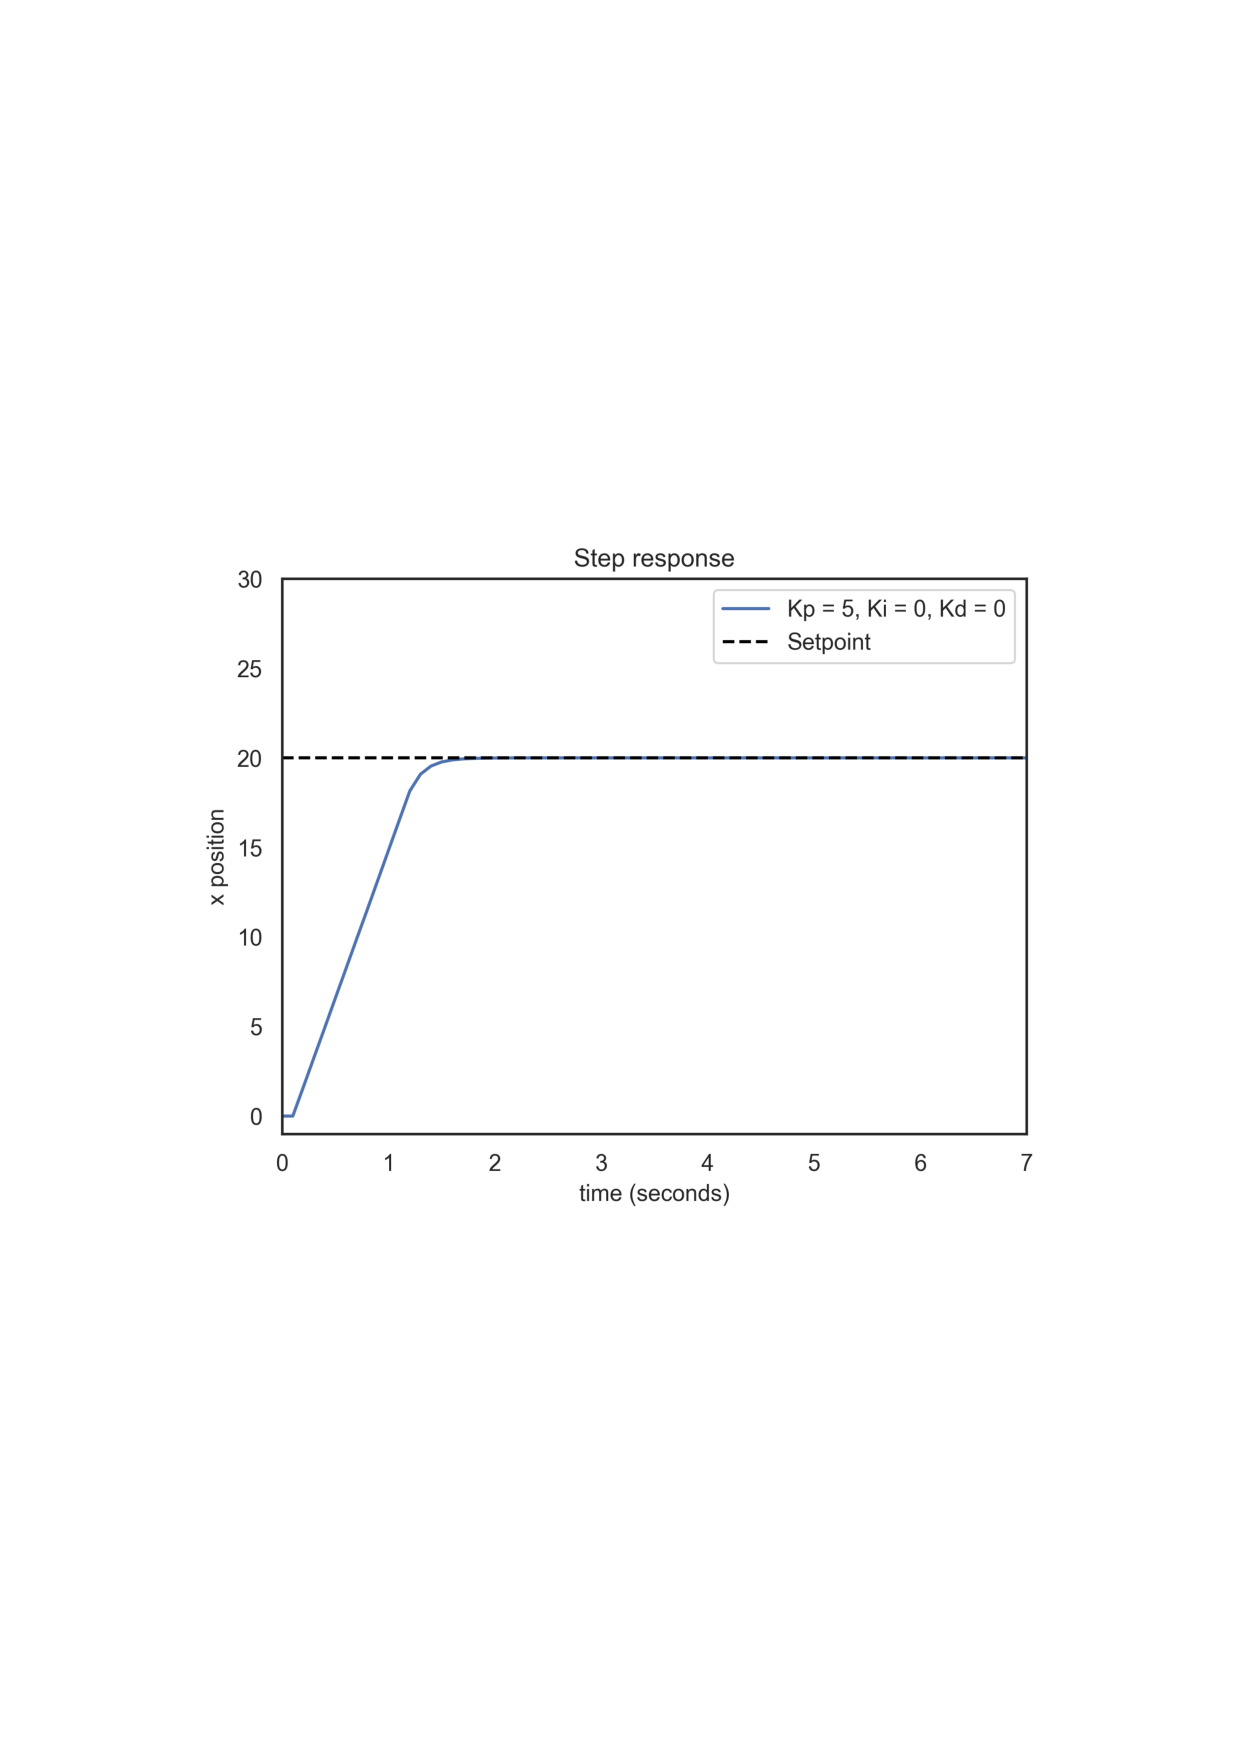
\includegraphics[width=.5\textwidth]{contents/images/Step-responsep=kp5ki0kd0}
	\caption[Step response of the proportinal PID controller.]{Visualisation of the 
	step-response of a P controller with proportional 
	gain $5$.}
	\label{fig:pid}
\end{figure}

It is important to notice that the speed returned by the controller is used to set the 
\texttt{motor\_\{left, right\}\_target}, both with the same value in order to move 
the robots straight ahead. Moreover, the first and the last robots of the line, 
whose sensors never receive a response respectively from the back and from the 
front, never move.

\subsection{Distributed approach}
\label{subsec:ex1distr}

\subsubsection{Experiments}
\label{subsubsec:expdist}

The first group of experiments we carried out, summarised in Table 
\ref{tab:modeln5dist}, examines the behaviour of the control learned in the case 
of the three different inputs, \texttt{prox\_values}, \texttt{prox\_comm} or 
\texttt{all\_sensors}, for a number of robots $N$ and an \texttt{avg\_gap} both 
fixed respectively at $5$ and the second chosen between $8$, $13$ and $24$.
\begin{figure}[!htb]
	\centering
	\begin{tabular}{cccc}
		\toprule
		\textbf{Model} \quad & \textbf{\texttt{network\_input}} & 
		\textbf{\texttt{input\_size}} &
		\textbf{\texttt{avg\_gap}} \\
		\midrule
		\texttt{net-d1} 				 & \texttt{prox\_values}	&  $  7$  &  $  8$  \\
		\texttt{net-d2} 				& \texttt{prox\_values}	    &  $  7$  &  $13$ \\
		\texttt{net-d3} 				& \texttt{prox\_values}	    &  $  7$  &  $24$  \\
		\texttt{net-d4} 				 & \texttt{prox\_comm}	  &  $  7$  &  $  8$  \\
		\texttt{net-d5} 				 & \texttt{prox\_comm}	  &  $  7$  &  $13$  \\
		\texttt{net-d6} 				 & \texttt{prox\_comm}	  &  $  7$  &  $24$  \\
		\texttt{net-d7} 				 & \texttt{all\_sensors}	  &  $14$  &  $  8$  \\
		\texttt{net-d8} 				 & \texttt{all\_sensors}	  &  $14$  &  $13$ 	\\
		\texttt{net-d9} 				 & \texttt{all\_sensors}	  &  $14$  &  $24$ 	\\
		\bottomrule
	\end{tabular}
	\captionof{table}[Experiments with $5$ agents (no communication).]{List of the 
	experiments carried out with $5$ agents.}
	\label{tab:modeln5dist}
\end{figure}

First of all we start by showing in Figure \ref{fig:distloss} an overview of the 
models performance in terms of train and validation losses. 
\begin{figure}[!htb]
	\centering
	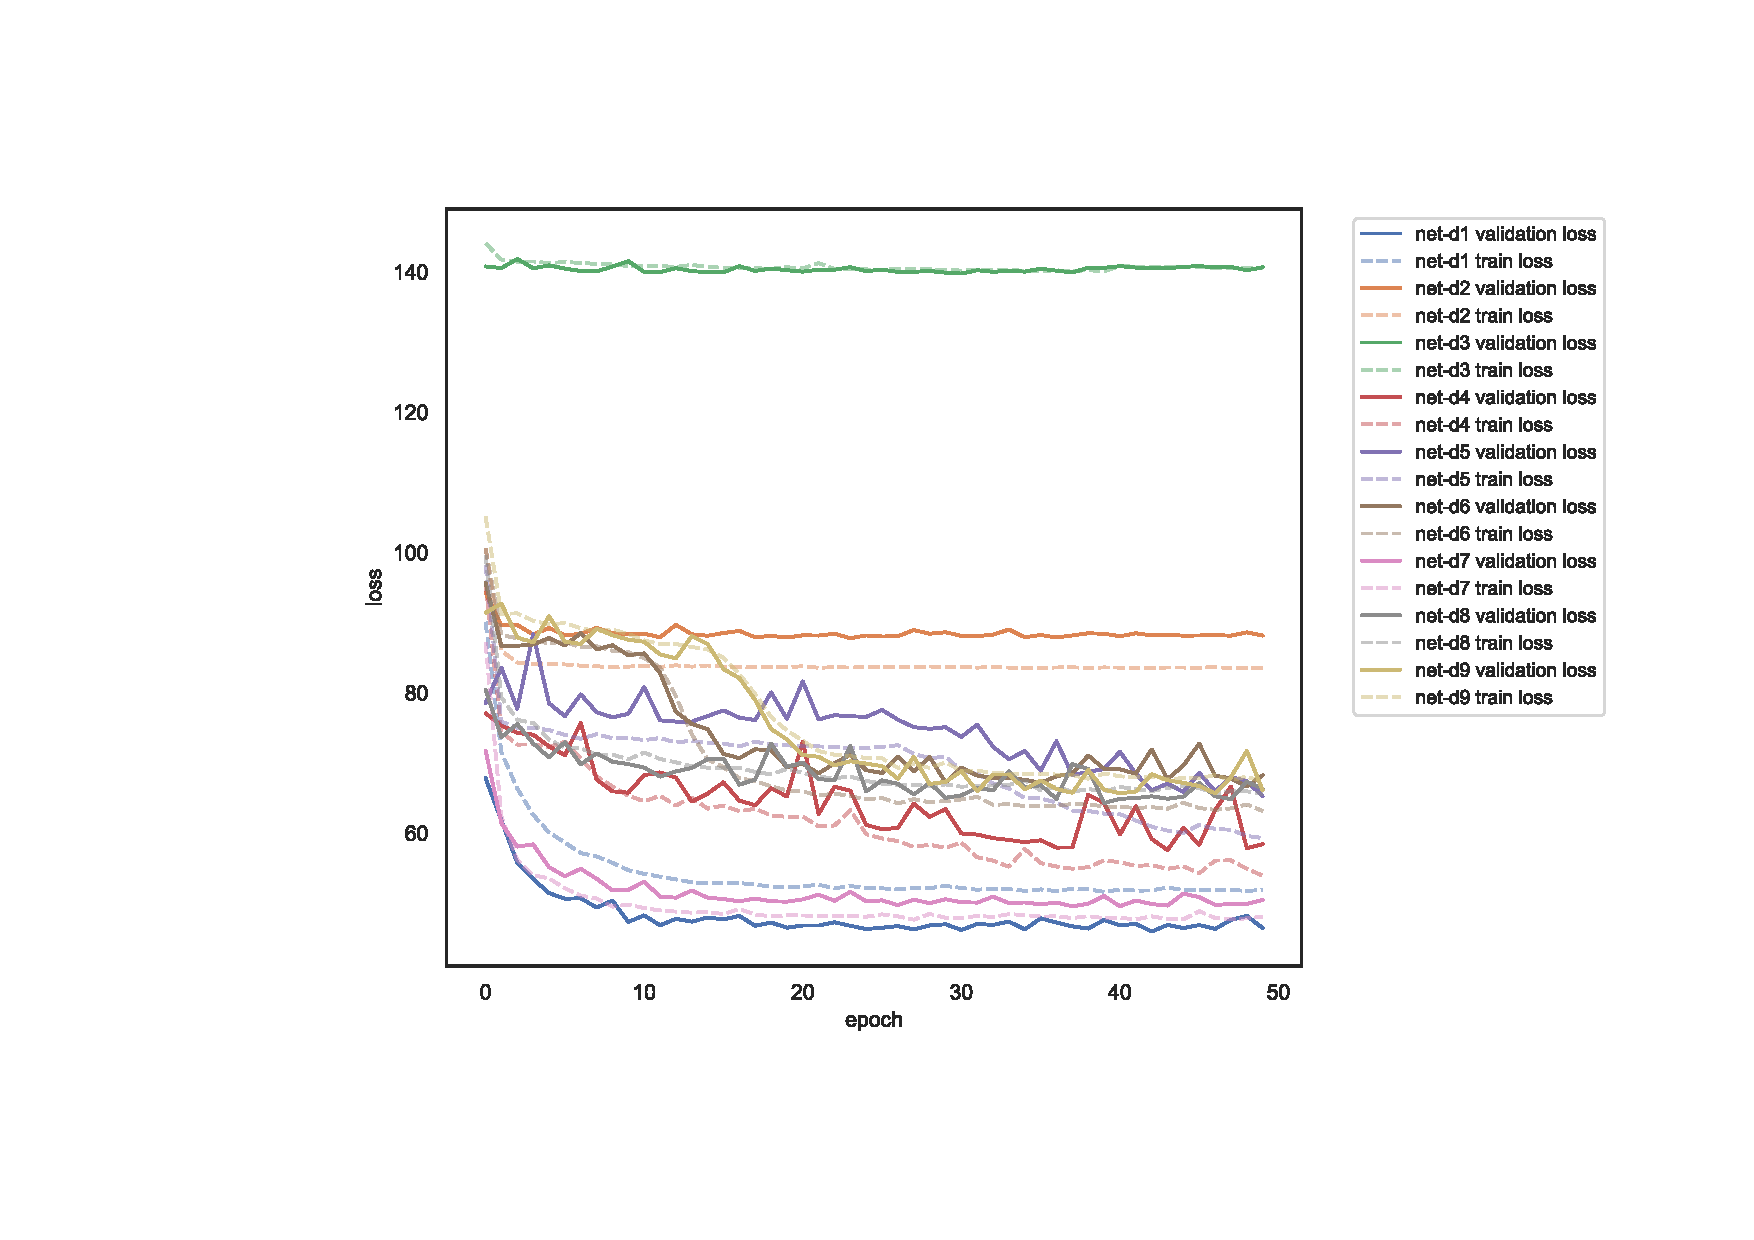
\includegraphics[width=.8\textwidth]{contents/images/task1/loss-distributed-all@}%
	\caption[Comparison of losses of the first set of 
	experiments.]{Comparison of 
	the losses of the models carried out with $5$ agents.}
	\label{fig:distloss}
\end{figure}
It is immediately evident that, in case of \texttt{prox\_values} inputs, the 
experiment performed with an \texttt{avg\_gap} of $24$ is not remarkable since 
the gap exceeds the maximal range of the sensor. In fact, from this analysis we 
generally expect a more stable behaviour using both types of input together, i.e. 
\texttt{all\_sensors}, as they are able to perform with both small and large gaps.

We start the analysis by exploring the results of the experiments obtained 
using the \texttt{prox\_values} readings alone as input of the network, continuing 
the with \texttt{prox\_comm} and concluding with \texttt{all\_sensors}.

The performance of \texttt{net-d1} are shown in the following images. In 
particular, in Figure \ref{fig:net-d1r2} is visualised a comparison of the \gls{r2}, 
or coefficient of determination, of the manual and the learned controllers, on the 
validation set.
This score function evidences how well the regression predictions approximate 
the real data points (groundtruth). Since a model which perfectly predicts the data 
has a score of $1$, we assume that a higher score corresponds to a model that 
performs better.
\begin{figure}[!htb]
	\centering
	\begin{subfigure}[h]{0.49\textwidth}
		\centering
		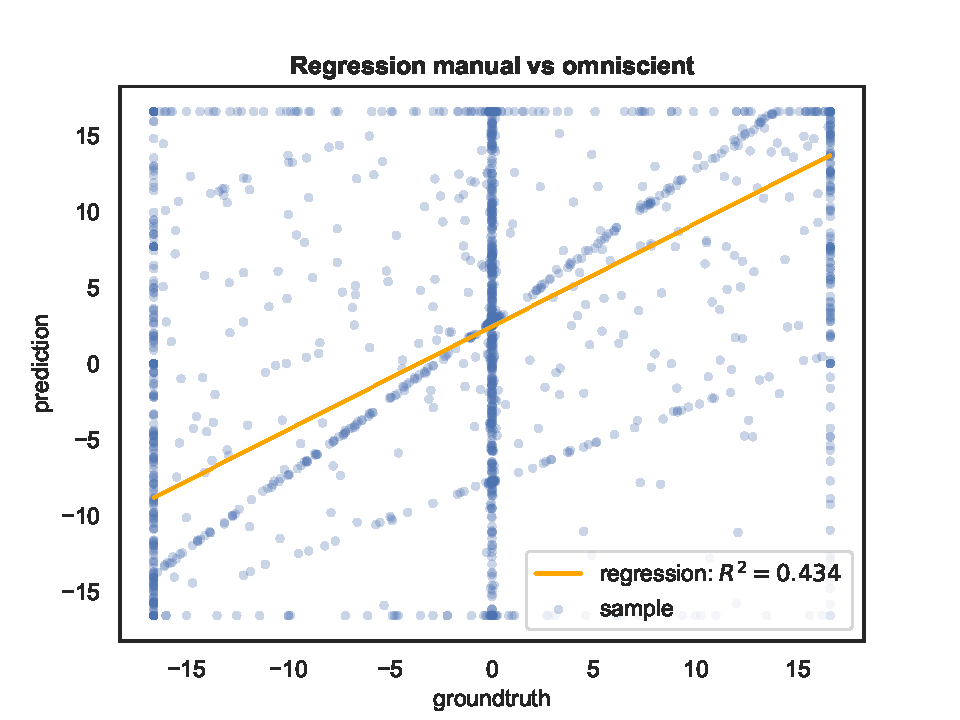
\includegraphics[width=\textwidth]{contents/images/net-d1/regression-manualvsomniscient}%
	\end{subfigure}
	\hfill
	\begin{subfigure}[h]{0.49\textwidth}
		\centering
		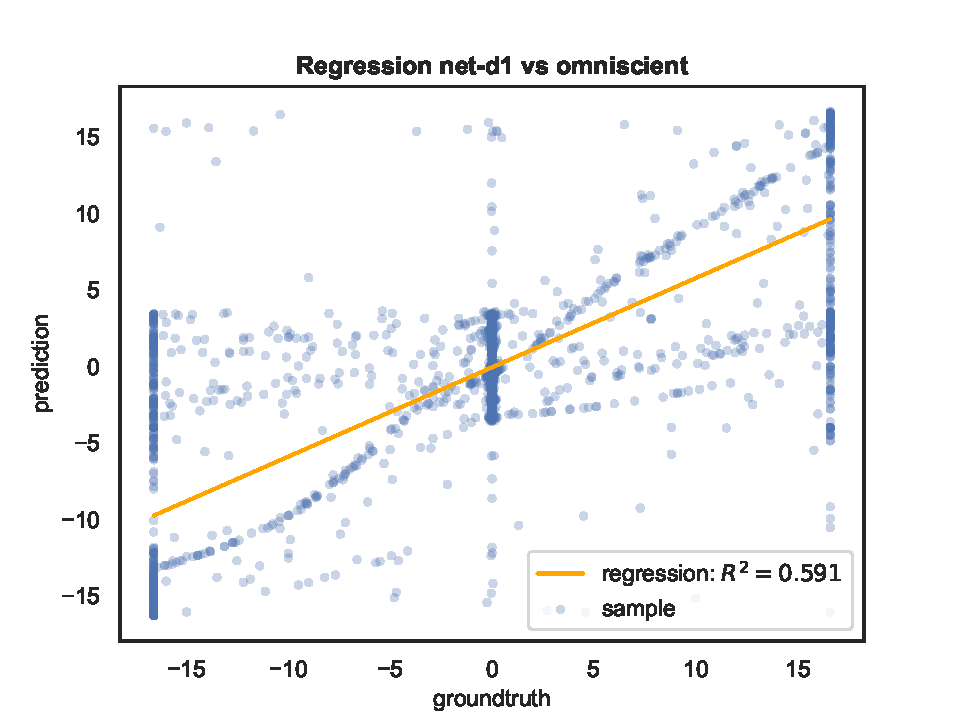
\includegraphics[width=\textwidth]{contents/images/net-d1/regression-net-d1-vs-omniscient}
	\end{subfigure}
	\caption[Evaluation of the \gls{r2} coefficients of \texttt{net-d1} 
	.]{Comparison of 
	the \gls{r2} coefficient of the manual and the controller learned from 
	\texttt{net-d1} with respect to the omniscient one.}
	\label{fig:net-d1r2}
\end{figure}
From these figures we expect that the robots' behaviour using the learned 
controller instead of the manual one is a bit better, even if far from the omniscient 
controller.

In Figure \ref{fig:net-d1traj} we first show a comparison of the expert and the 
learned trajectories, and then between the manual and the learned ones. In 
particular, on the y-axis is visualised the position of each agent over time, while 
on the x-axis the simulation time steps. It is important to notice that the plots 
summarise all the validation runs: at each time step, the position of each agent is 
presented as an average over all the simulation runs, and besides is shown this 
average minus and plus the standard deviation.
\begin{figure}[!htb]
	\begin{center}
		\begin{subfigure}[h]{0.49\textwidth}
			\centering
			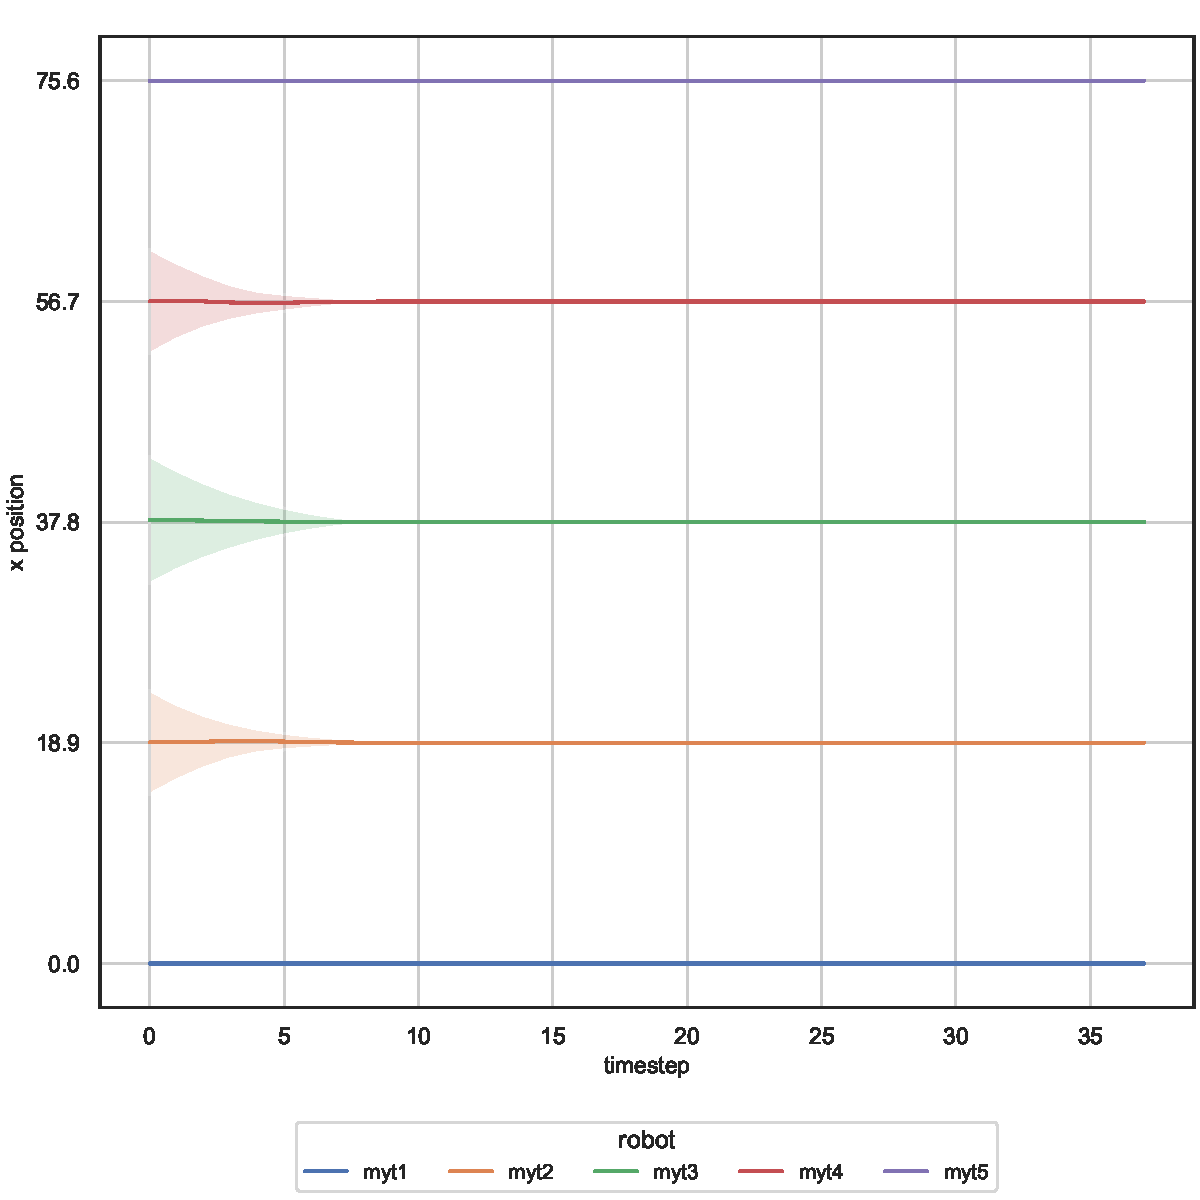
\includegraphics[width=.9\textwidth]{contents/images/net-d1/position-overtime-omniscient}%
			\caption{Expert controller trajectories.}
		\end{subfigure}
		\hfill
		\begin{subfigure}[h]{0.49\textwidth}
			\centering
			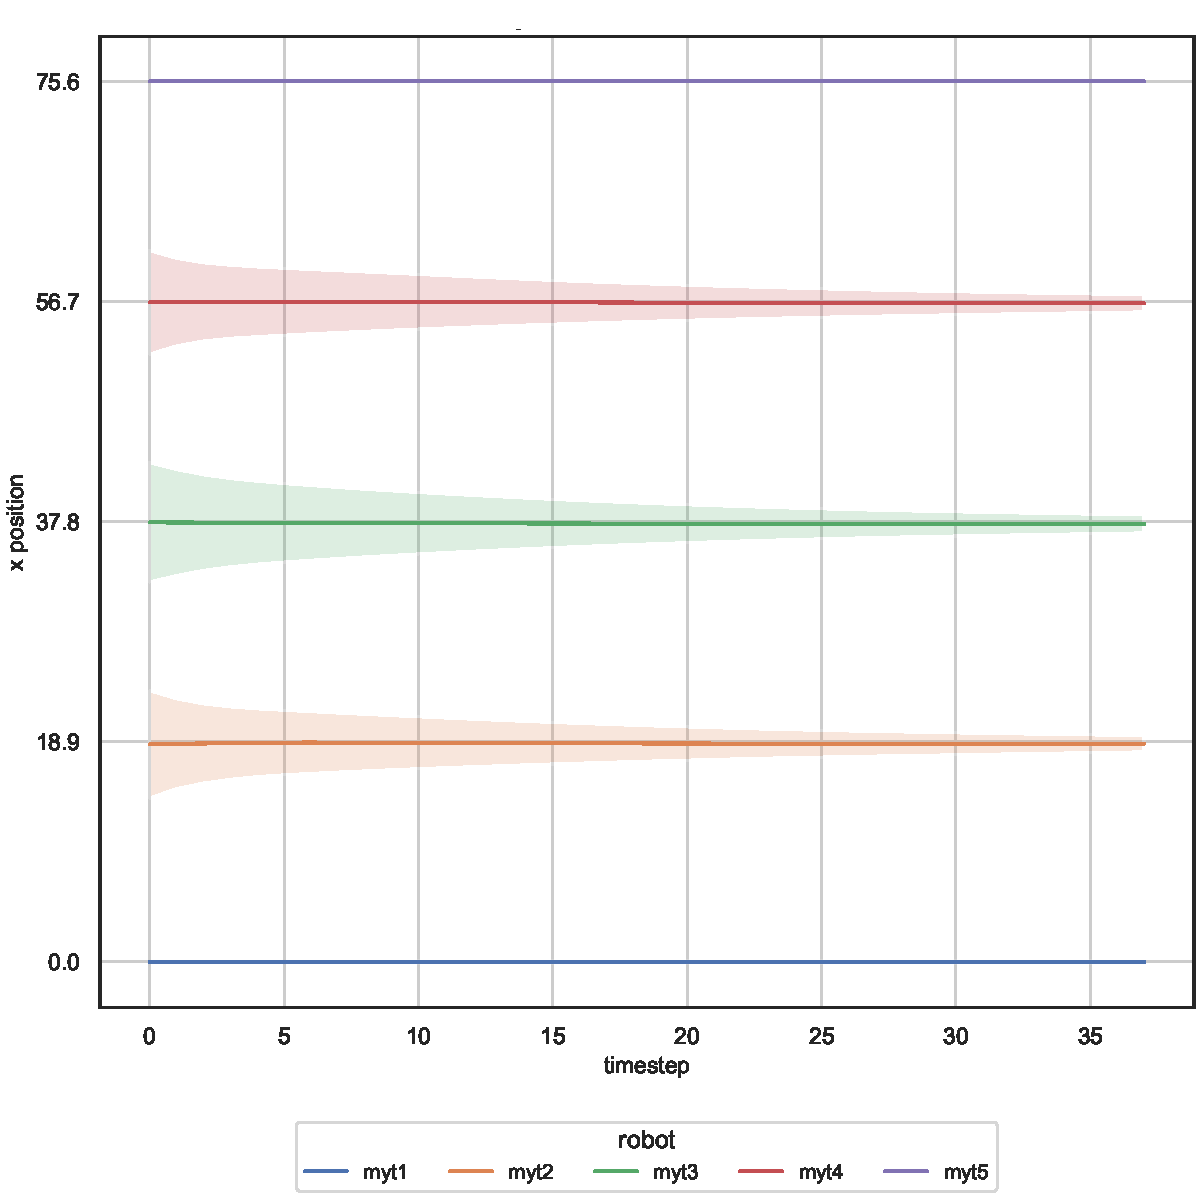
\includegraphics[width=.9\textwidth]{contents/images/net-d1/position-overtime-learned_distributed}
			\caption{Distributed controller trajectories.}
		\end{subfigure}
	\end{center}
	\begin{center}  
		\begin{subfigure}[h]{0.49\textwidth}
			\centering
			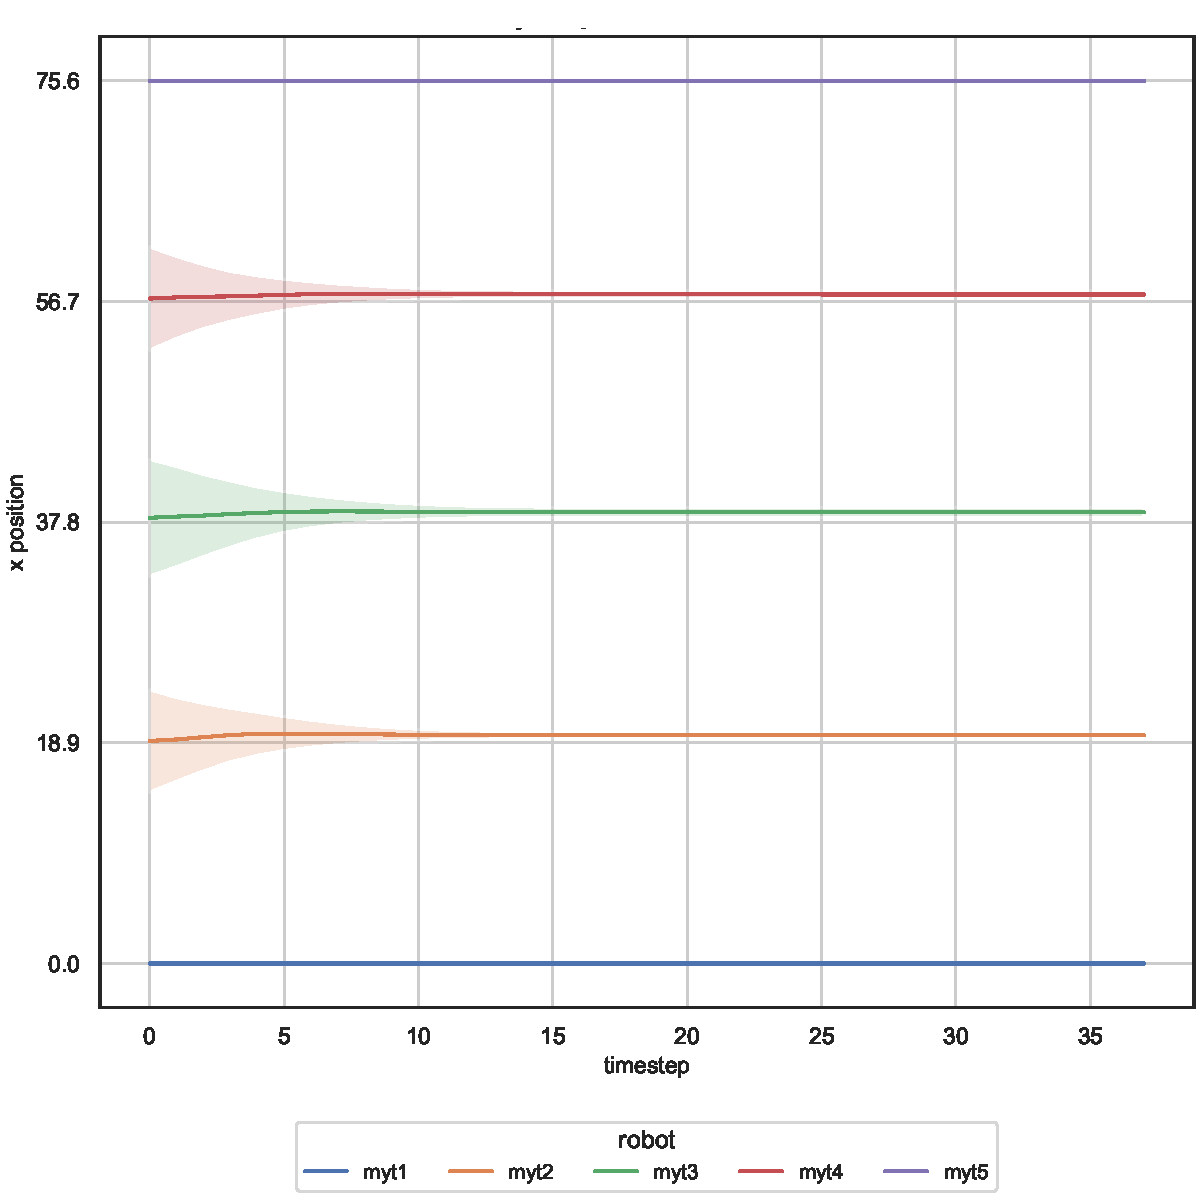
\includegraphics[width=.9\textwidth]{contents/images/net-d1/position-overtime-manual}%
			\caption{Manual controller trajectories.}
		\end{subfigure}
		\hfill
		\begin{subfigure}[h]{0.49\textwidth}
			\centering
			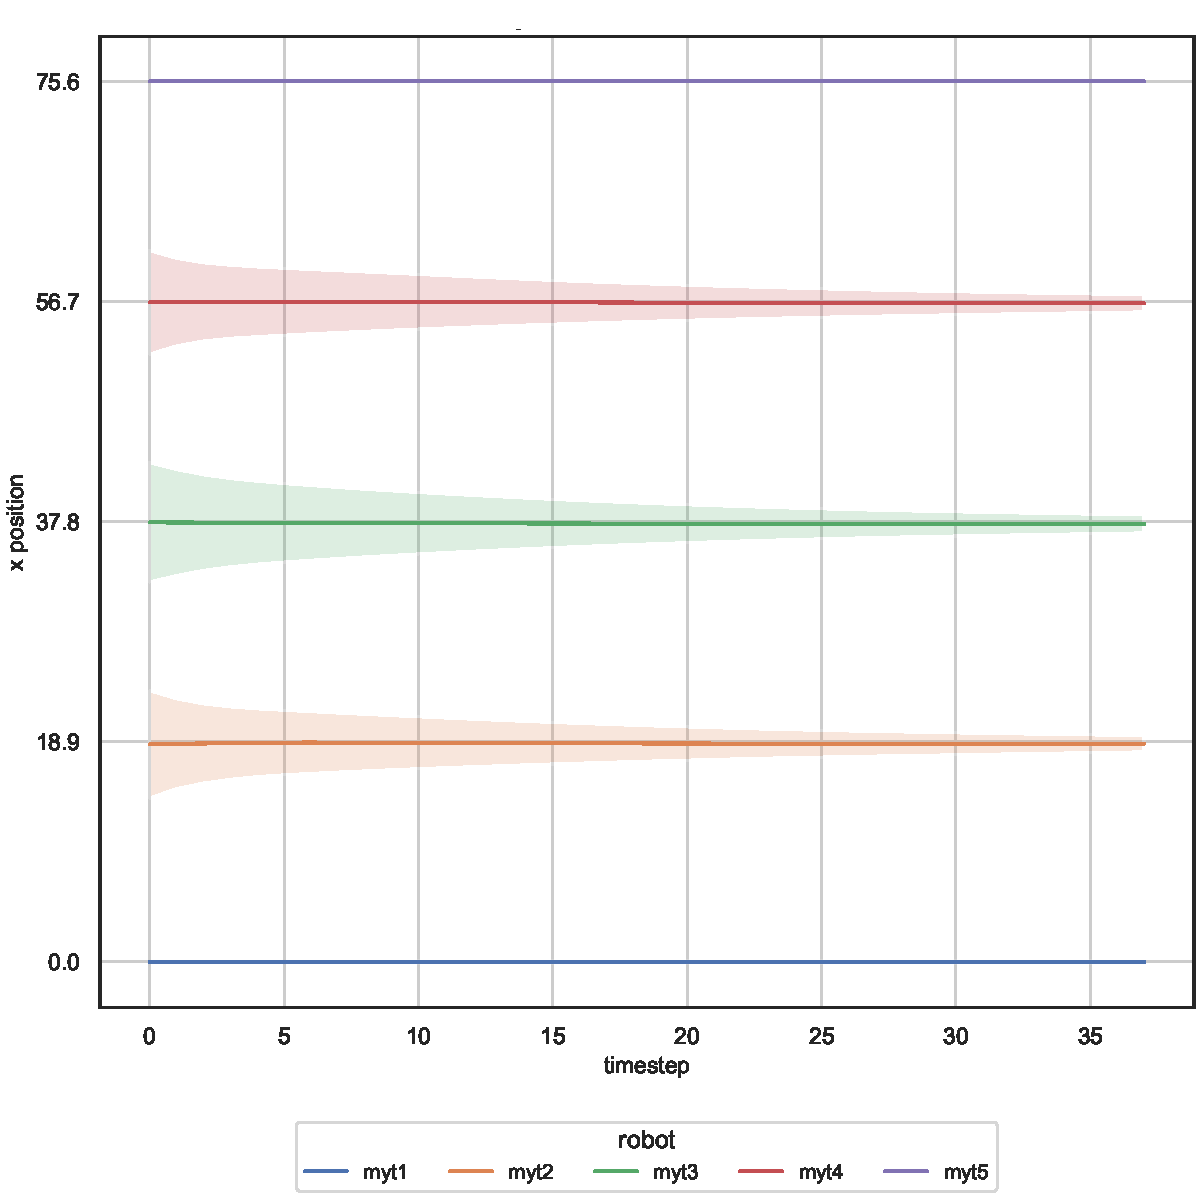
\includegraphics[width=.9\textwidth]{contents/images/net-d1/position-overtime-learned_distributed}
			\caption{Distributed controller trajectories.}
		\end{subfigure}
	\end{center}
	\caption[Evaluation of the trajectories learned by \texttt{net-d1}.]{Comparison 
		of trajectories generated using three controllers: the expert, the manual and 
		the one learned from \texttt{net-d1}.}
	\label{fig:net-d1traj}
\end{figure}
The convergence of the robots to the target using the omniscient controller is 
much faster that with the manual or the learned one. Generally the learned 
trajectories require a higher number of time steps to converge to the correct 
configuration, sometimes even $40$ may be necessary, compared to the two 
others controllers that need less than $10$ time steps.

Indeed, analysing in Figure \ref{fig:net-d1control} the evolution of the control 
over time, it is possible to notice that the omniscient in the first time steps uses a 
higher speed than that chosen by the manual controller or the one predicted by 
the network. 
\begin{figure}[!htb]
	\centering
	\begin{subfigure}[h]{0.3\textwidth}
		\centering
		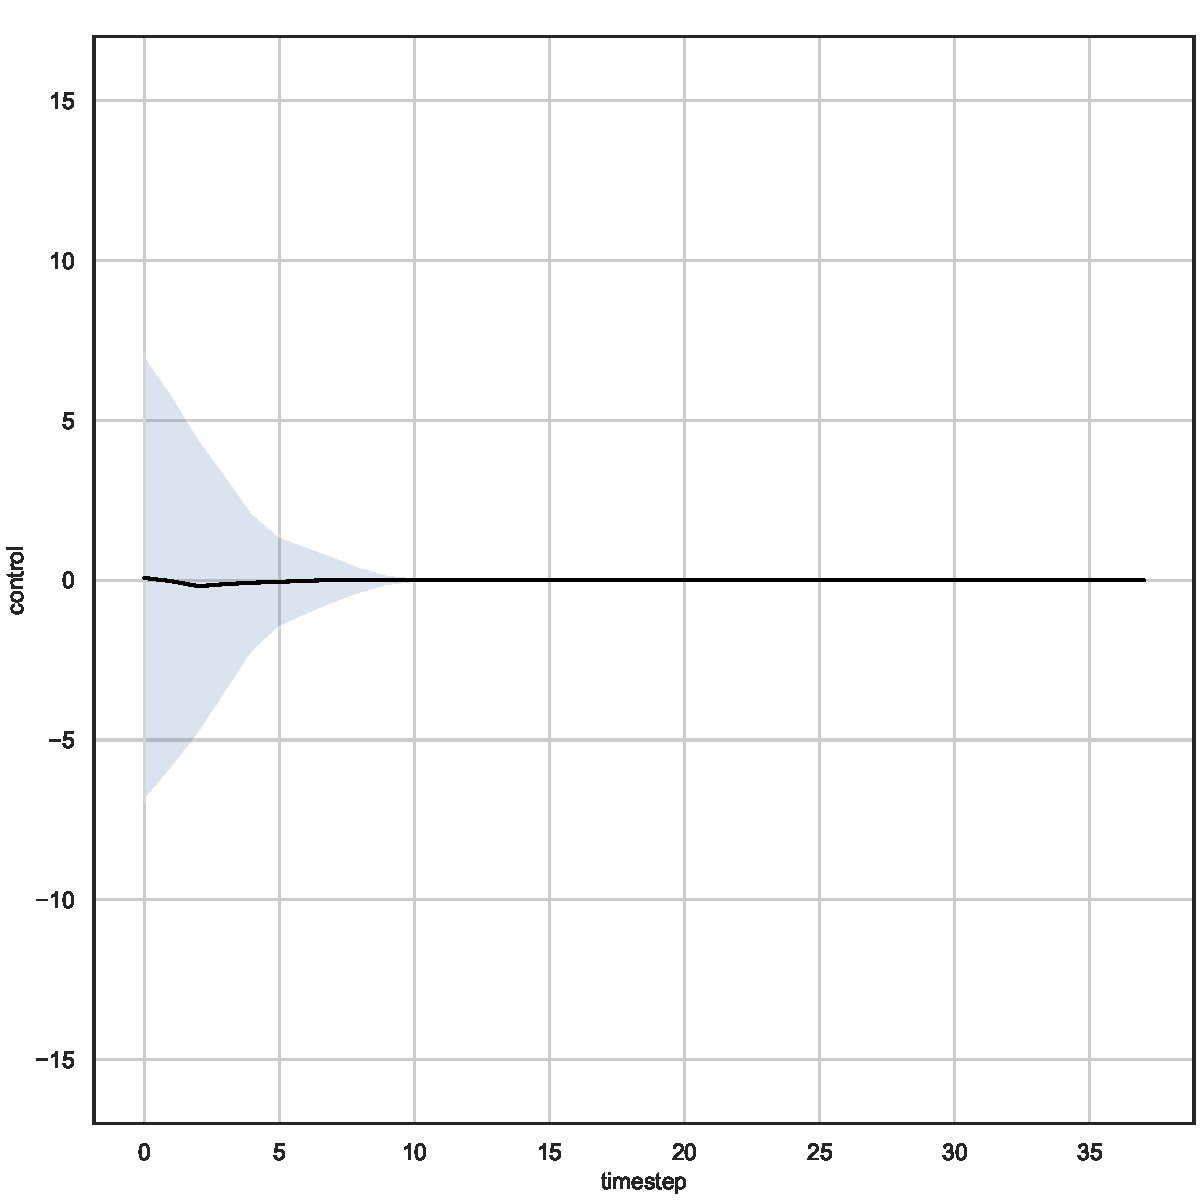
\includegraphics[width=\textwidth]{contents/images/net-d1/control-overtime-omniscient}%
		\caption{Expert controller.}
	\end{subfigure}
	\hfill
	\begin{subfigure}[h]{0.3\textwidth}
		\centering
		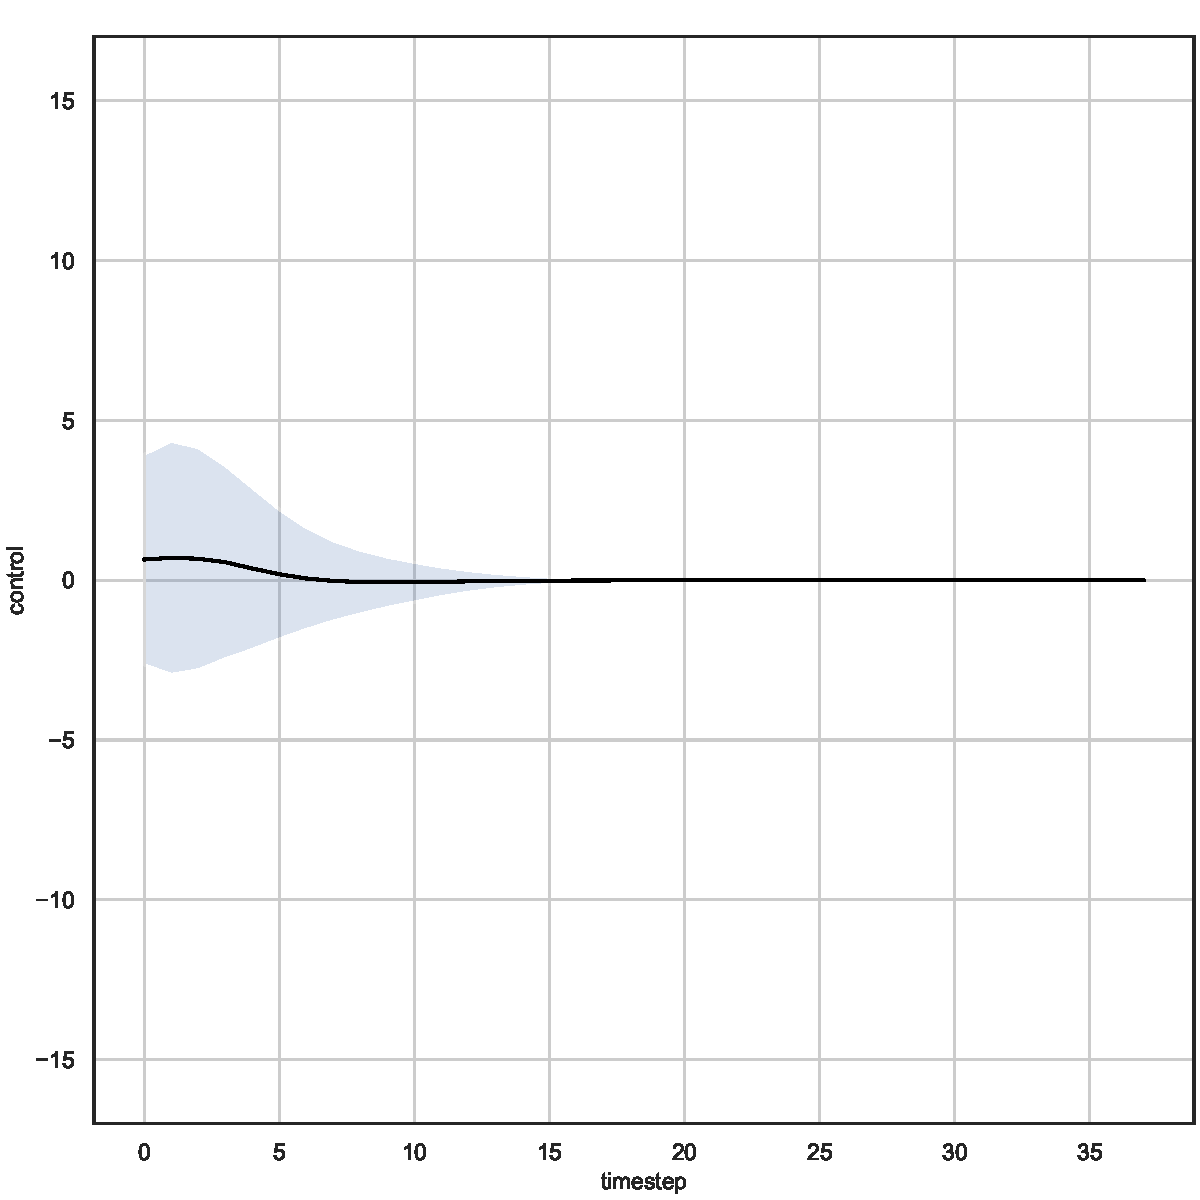
\includegraphics[width=\textwidth]{contents/images/net-d1/control-overtime-manual}%
		\caption{Manual controller.}
	\end{subfigure}
	\hfill
	\begin{subfigure}[h]{0.3\textwidth}
		\centering
		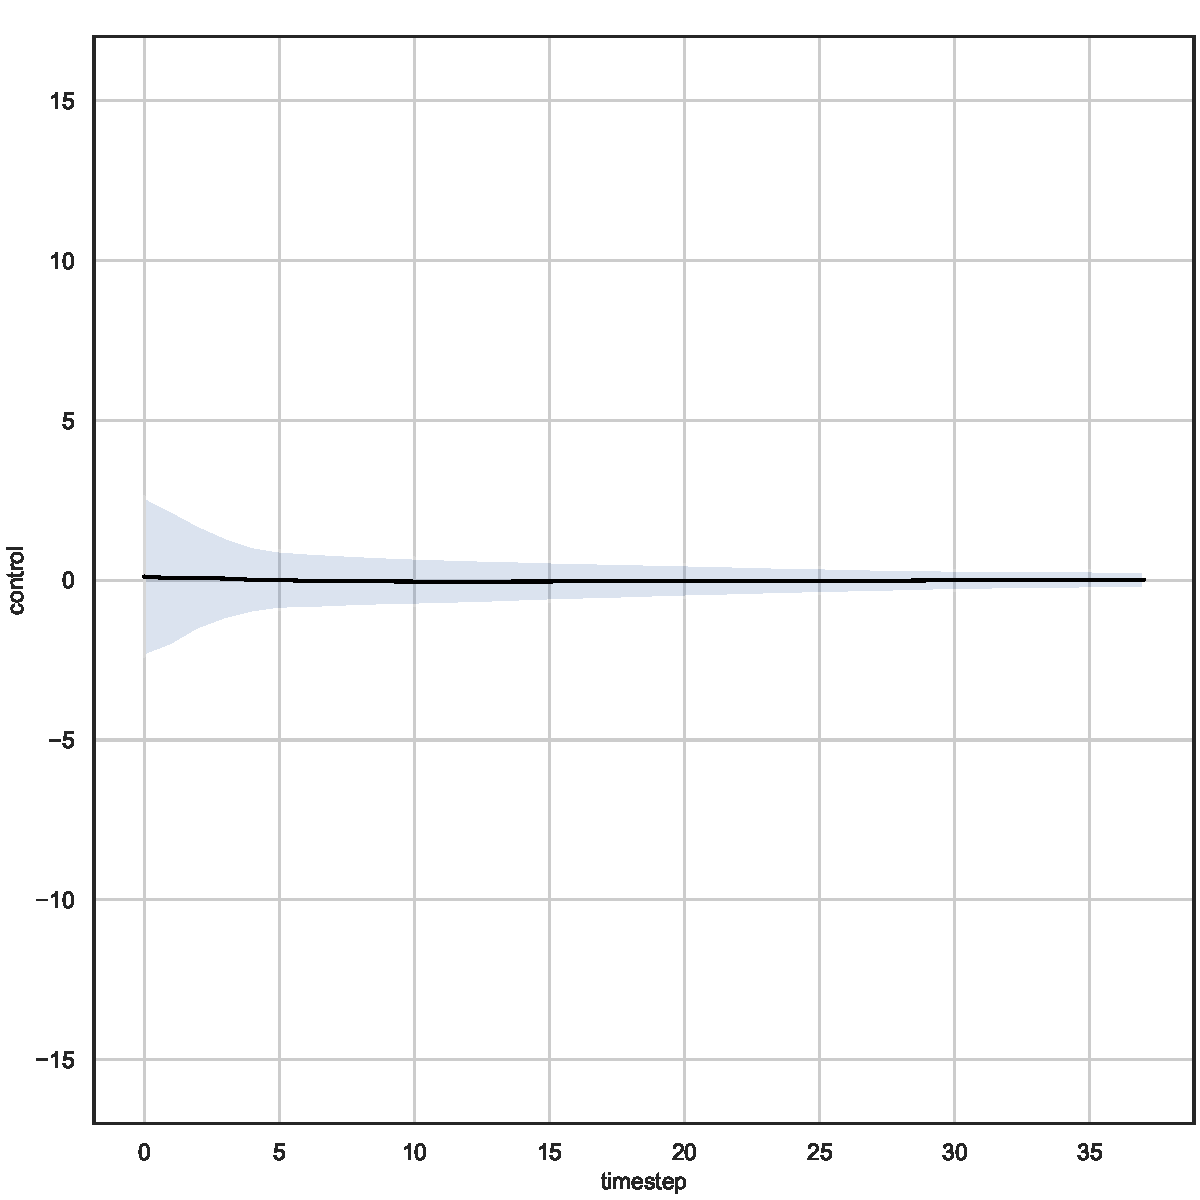
\includegraphics[width=\textwidth]{contents/images/net-d1/control-overtime-learned_distributed}
		\caption{Distributed controller.}
	\end{subfigure}
	\caption[Evaluation of the control learned by \texttt{net-d1}.]{Comparison 
		of output control decided using three controllers: the expert, the manual 
		and the one learned from \texttt{net-d1}.}
	\label{fig:net-d1control}
\end{figure}
After about $10$ time steps the expert reaches the target while the manual need 
about $15$ time steps to arrive to the goal with a certain tolerance, maintaining 
then the speed constant at $0$. Instead, the distributed controller decreases the 
speed of the agents as the time steps pass, reaching zero speed but with a certain 
variance, probably caused by oscillations.

\bigskip
\bigskip
A couple of useful plots are shown below. In Figure 
\ref{fig:net-d1responsesensors} is visualised the response of the learned 
controller as the input sensing changes. 
\begin{figure}[!htb]
	\centering
	\begin{subfigure}[h]{0.49\textwidth}
		\centering
		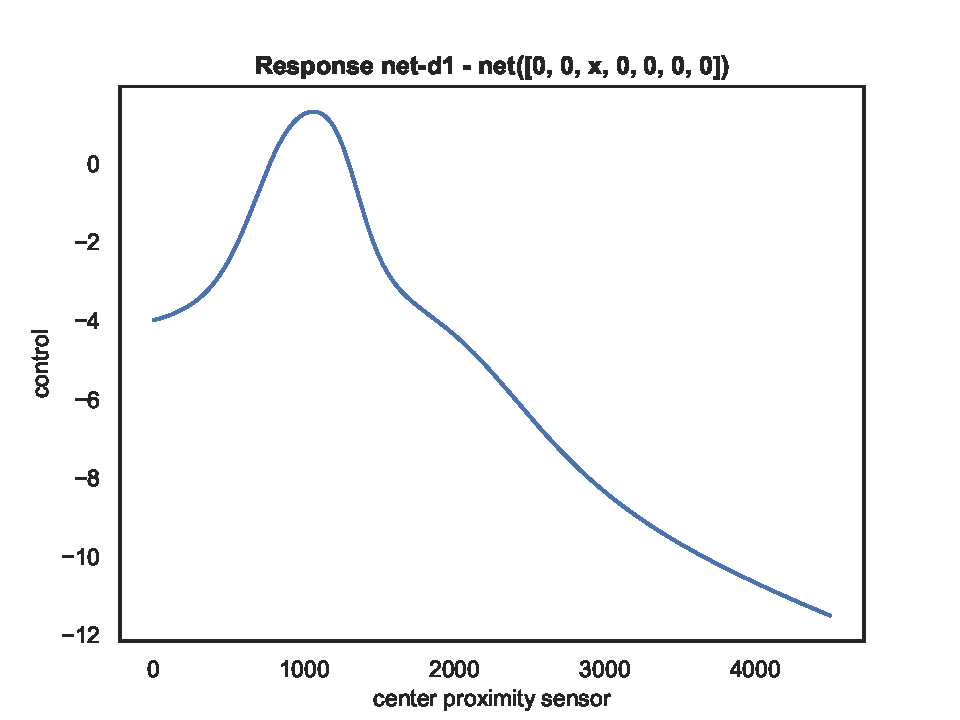
\includegraphics[width=\textwidth]{contents/images/net-d1/response-net-d1-front}%
		%\caption{response-net-d1-net([0, 0, x, 0, 0, 0, 0]).}
	\end{subfigure}
	\hfill
	\begin{subfigure}[h]{0.49\textwidth}
		\centering
		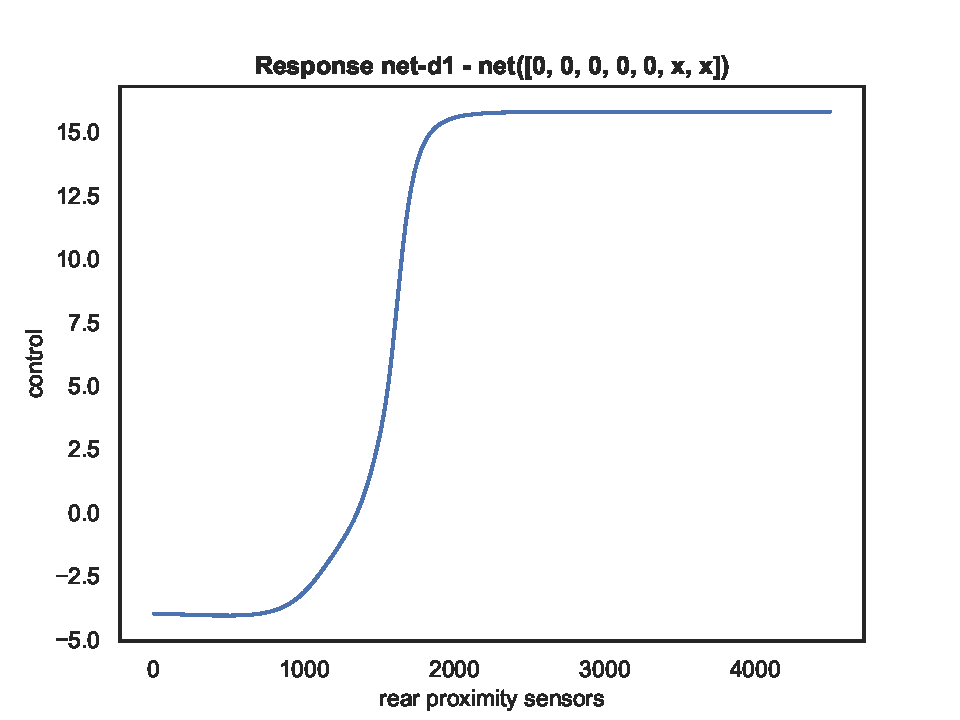
\includegraphics[width=\textwidth]{contents/images/net-d1/response-net-d1-rear}
		%\caption{response-net-d1-net([0, 0, 0, 0, 0, x, x]).}
	\end{subfigure}
	\caption[Response of \texttt{net-d1} by varying the input sensing.]{Response of 
		\texttt{net-d1} by varying the input sensing.}
	\label{fig:net-d1responsesensors}
\end{figure}
In particular we analyse two cases. The first one shows the control predicted by 
the network when the robot sees only in front and nothing behind, more 
specifically when the given input is  $([0, 0, x, 0, 0, 0, 0])$, with $x$ varying in the 
range $[0, 4500]$.
The second shows the control predicted by the network when the robot instead 
sees nothing in front, more specifically when the given input is  $([0, 0, 0, 0, 0,x , 
x])$, with $x$ varying in the range $[0, 4500]$.
The behaviour is almost as expected. When the robot sees nothing behind but 
something in front, the model returns a negative speed, since the robot has to 
move backwards. 
The absolute value of control increases as the proximity to the obstacle increases.
A complementary behaviour is obtained when the robot sees only behind but 
not in front.

\begin{figure}[!htb]
	\centering
	\includegraphics[width=.45\textwidth]{contents/images/net-d1/response-varying_init_position-distributed}%
	\caption{Response of \texttt{net-d1} by varying the initial position.}
	\label{fig:net-d1responseposition}
\end{figure}
In Figure \ref{fig:net-d1responseposition} is displayed the behaviour of a robot 
located between two stationary agents which are already in their place, showing 
the response of the controllers, on the y-axis, by varying the position of the 
moving robot, visualised on the x-axis. The output control is computed as an 
average over $100$ measures in which the pose of the agent $(x, y, \theta)$ 
differs by a certain epsilon uniformly distributed in the range $[-0.5, 0.5]$, thus 
to avoid the effects of noise that would be obtained on a single measurement and 
unrealistic artefacts in which the sensors are not continuous. Besides, are shown 
the bands which represent plus and minus standard deviation. As expected, the 
output is a high value, positive or negative respectively when the robot is close to 
an obstacle on the left or on the right, or it is close to $0$ when the distance from 
right and left is equal.
\begin{figure}[H]
	\centering
	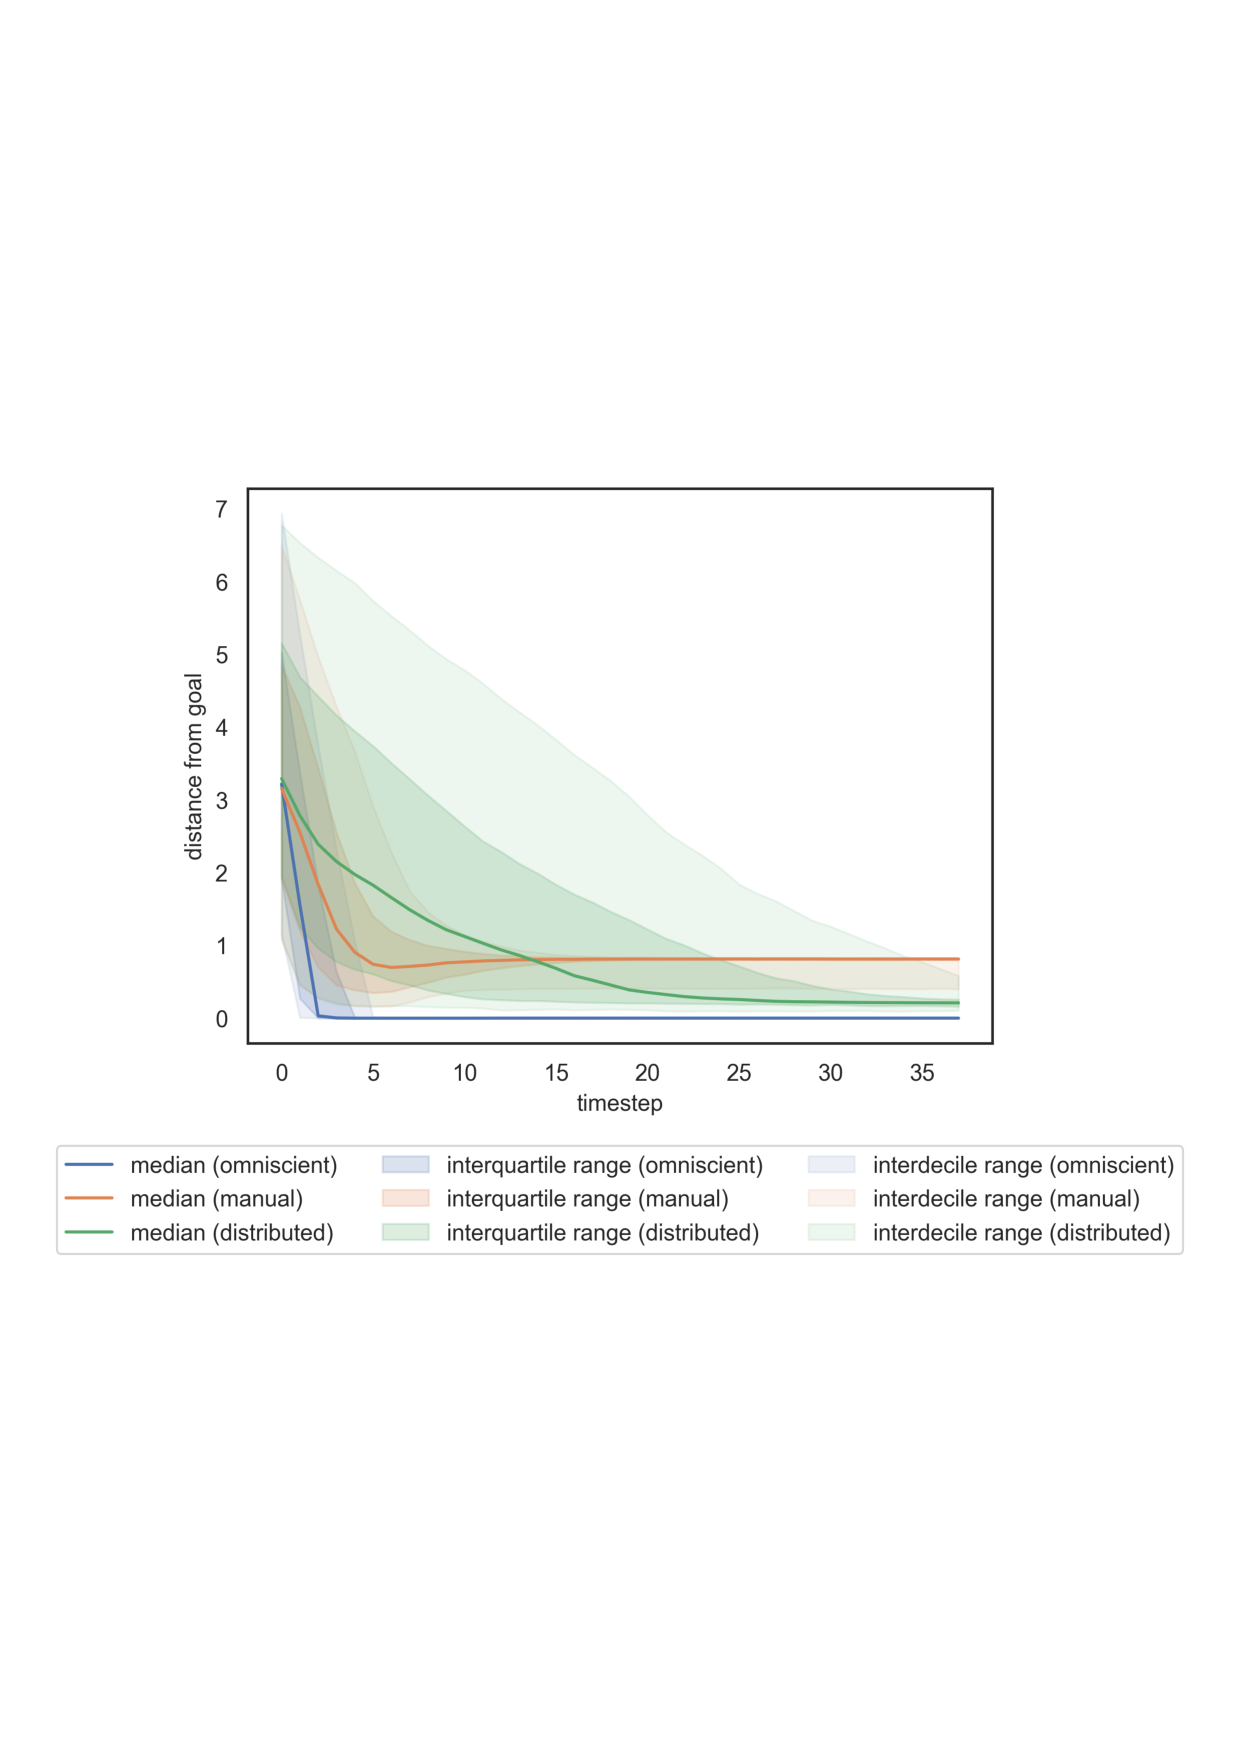
\includegraphics[width=.65\textwidth]{contents/images/net-d1/distances-from-goal-compressed-distributed}%
	\caption[Evaluation of \texttt{net-d1} distances from goal.]{Comparison of 
		performance in terms of distances from goal obtained using three 
		controllers: 
		the expert, the manual and the one learned from \texttt{net-d1}.}
	\label{fig:net-d1distance}
\end{figure}

Finally, in Figure \ref{fig:net-d1distance} is presented another useful metric that 
measures the absolute distance of each robot from the target, visualised on the 
y-axis, over time. This value is averaged on all robots among all the simulation 
runs. The median value is shown as well as the interquartile and interdecile ranges.
On average, the distance from goal of the learned controller is lower than the one 
obtained with the manual controller, meaning that in the final configuration 
the robots moved following the learned controller are closer to the target than 
those moved with the manual one, which are on average at a distance of about 
$1$\gls{cm} from the goal position. 

As mentioned before, in case of \texttt{prox\_values} inputs the 
experiment performed with an \texttt{avg\_gap} of $24$ is not meaningful since 
this value exceeds the maximal range of the sensor. Similarly, since $14$ is the 
maximum range, it is difficult to use this type of input when the \texttt{avg\_gap}  
is $13$, as shown by the losses in Figure \ref{fig:distlossprox_values}.
\begin{figure}[!htb]
	\centering
	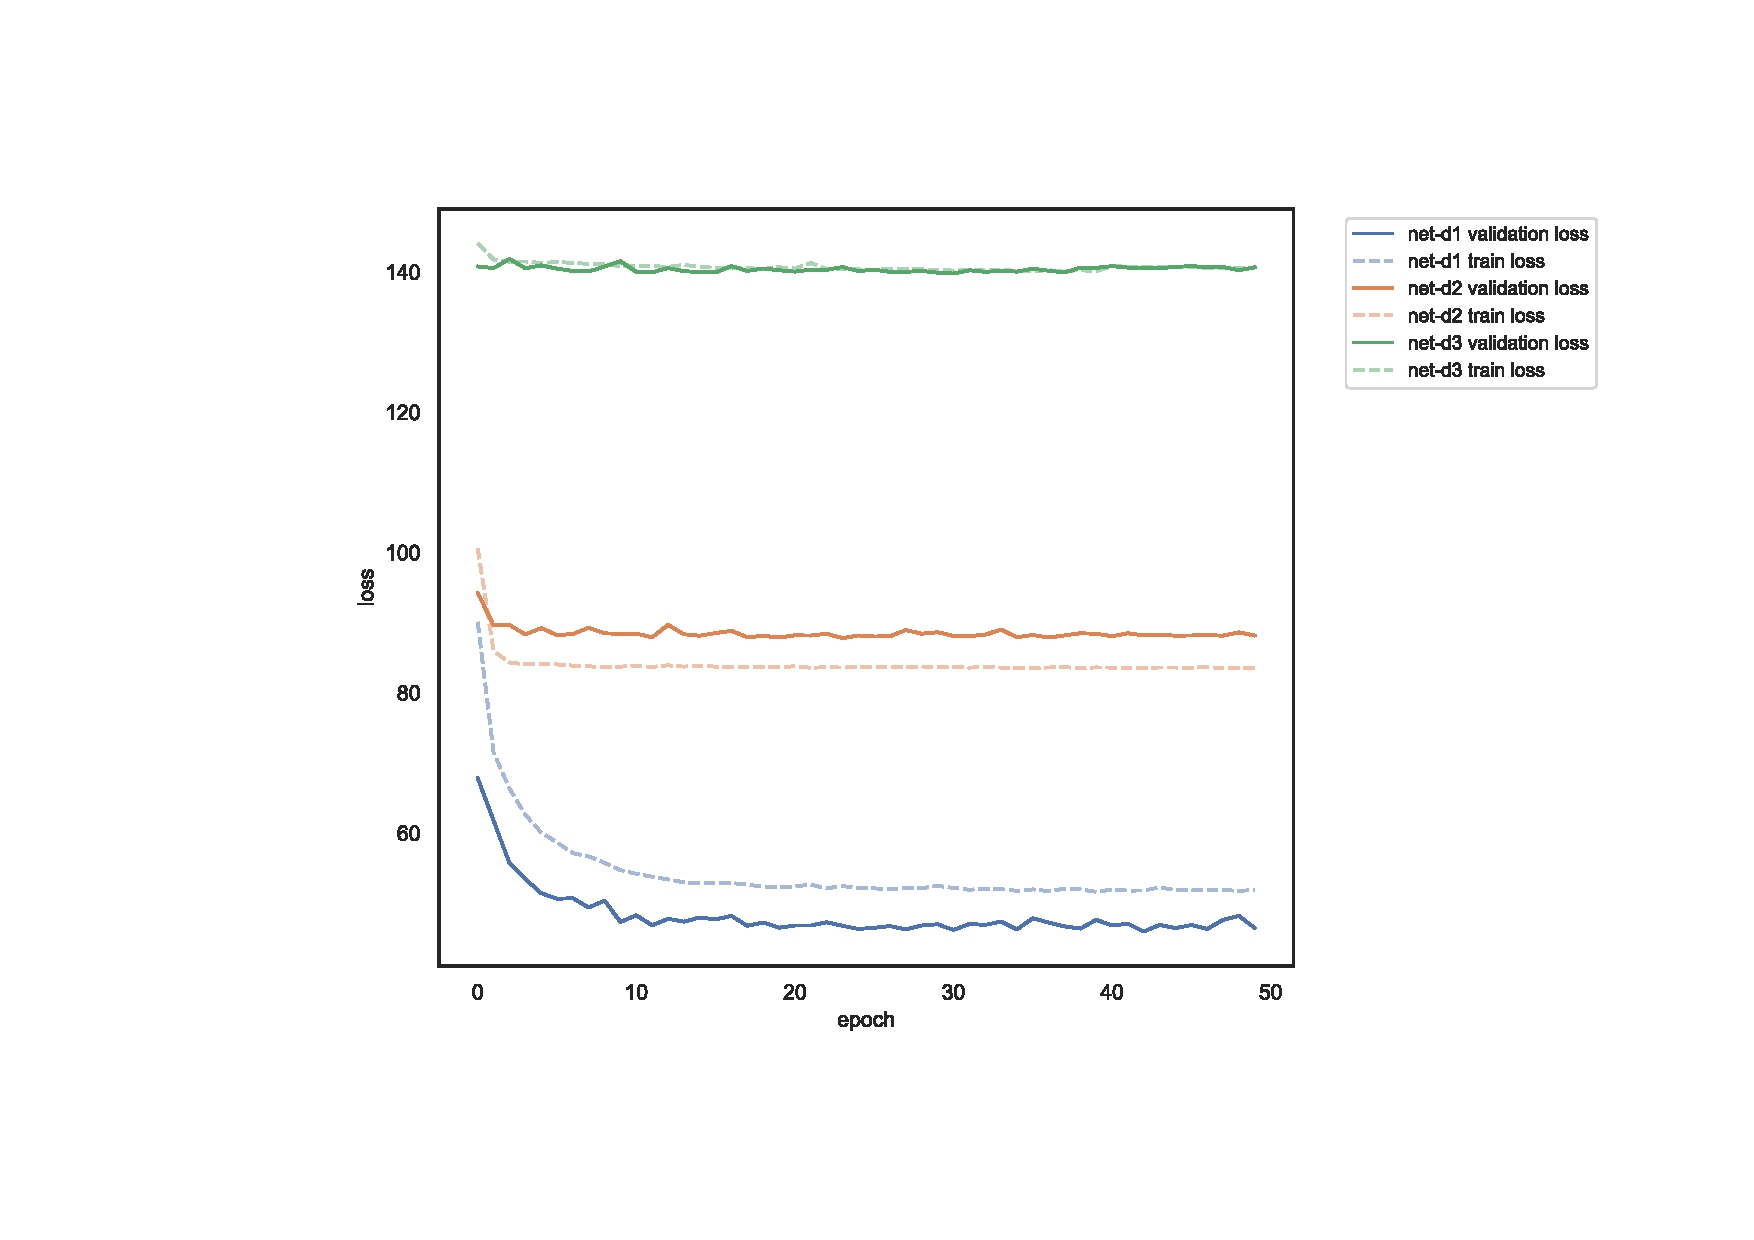
\includegraphics[width=.8\textwidth]{contents/images/task1/loss-distributed-prox_values@}%
	\caption{Comparison of the losses of the models that use \texttt{prox\_values} 
		readings.}
	\label{fig:distlossprox_values}
\end{figure}

Following are shown the results of the experiments obtained using the 
\texttt{prox\_comm} readings. 
\begin{figure}[!htb]
	\centering
	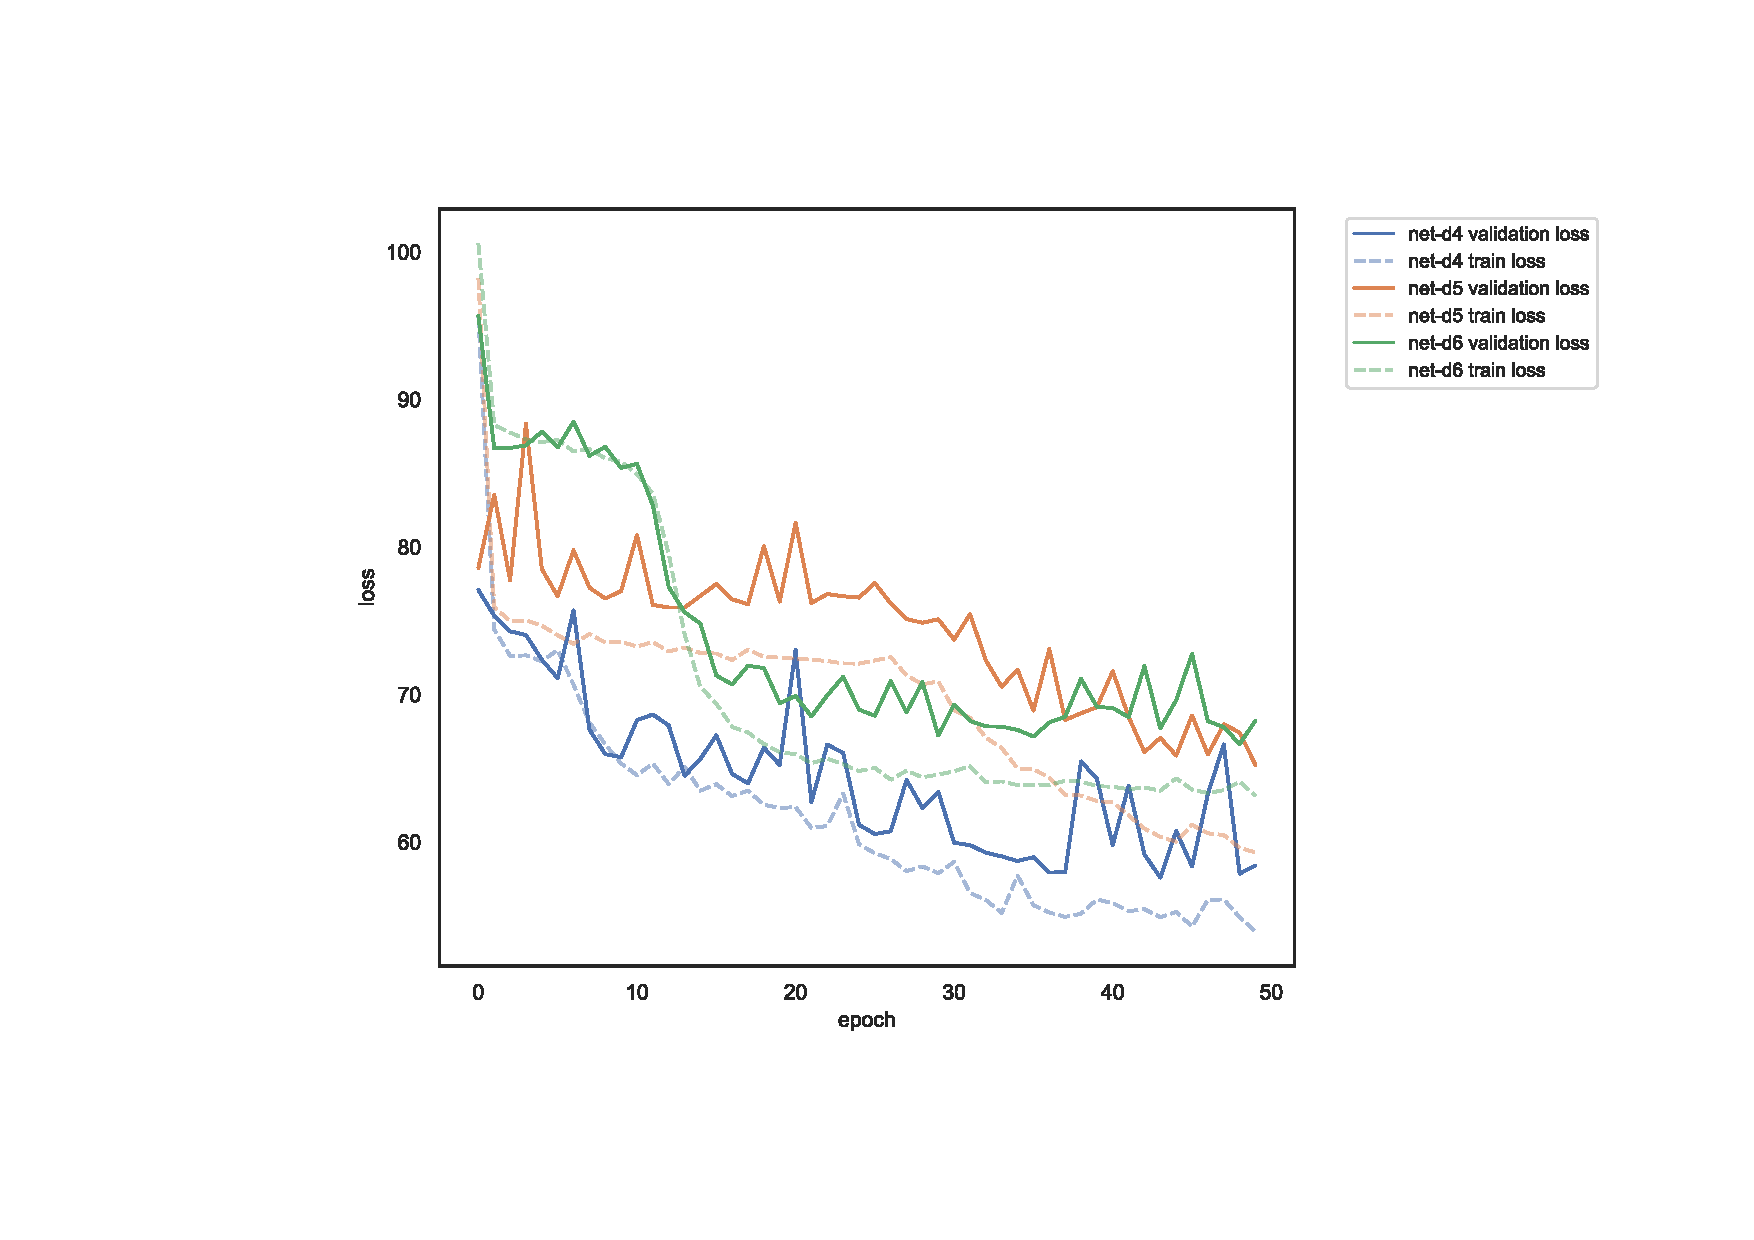
\includegraphics[width=.8\textwidth]{contents/images/task1/loss-distributed-prox_comm@}%
	\caption{Comparison of the losses of the models that use \texttt{prox\_comm} 
		readings.}
	\label{fig:distlossprox_comm}
\end{figure}
In Figure \ref{fig:distlossprox_comm}, are analysed the losses by varying the 
average gap. From a first observation the network seems to be able to work with 
all the gaps.

Examining the \gls{r2} coefficients in Figure \ref{fig:net-d456r2}, the higher 
value is obtained with \texttt{net-d6}. For the assumptions made before we 
believe that this model is more promising. 
\begin{figure}[!htb]
	\begin{center}
		\begin{subfigure}[h]{0.49\textwidth}
			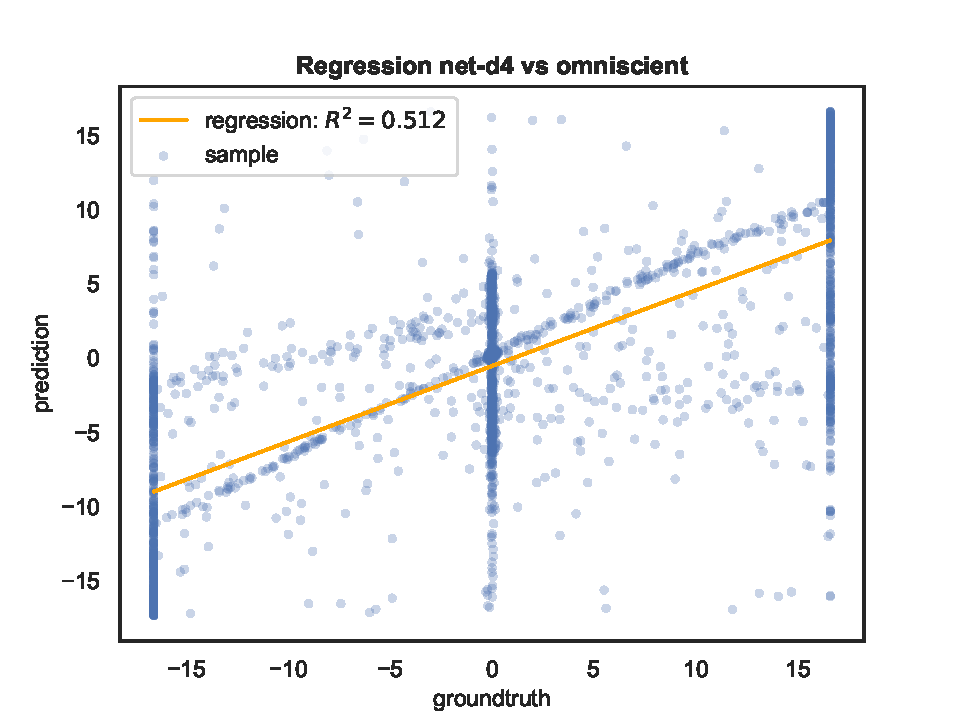
\includegraphics[width=\textwidth]{contents/images/net-d4/regression-net-d4-vs-omniscient}%
		\end{subfigure}
		\hfill\vspace{-0.5cm}
		\begin{subfigure}[h]{0.49\textwidth}
			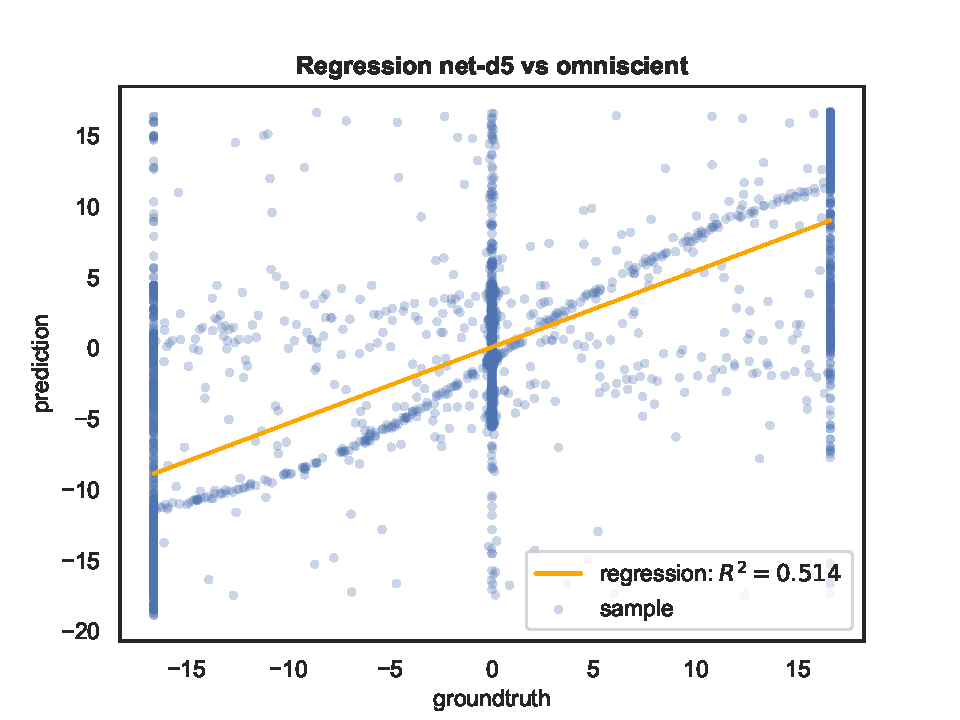
\includegraphics[width=\textwidth]{contents/images/net-d5/regression-net-d5-vs-omniscient}%
		\end{subfigure}
	\end{center}
	\begin{center}
		\begin{subfigure}[h]{0.49\textwidth}
			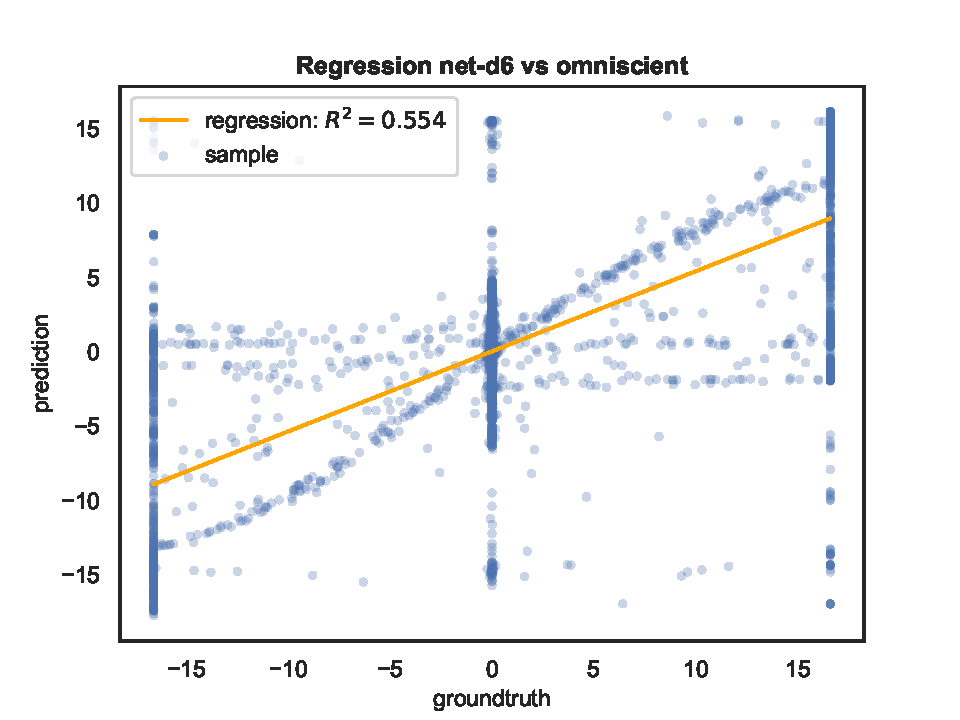
\includegraphics[width=\textwidth]{contents/images/net-d6/regression-net-d6-vs-omniscient}
		\end{subfigure}
	\end{center}
	\caption[Comparison of the \gls{r2} coefficients for \texttt{prox\_comm} 
	readings.]{Comparison of the \gls{r2} coefficients of the models that use 
	\texttt{prox\_comm} readings.}
	\label{fig:net-d456r2}
\end{figure}
\begin{figure}[H]
	\centering
	\begin{subfigure}[h]{0.49\textwidth}
		\centering
		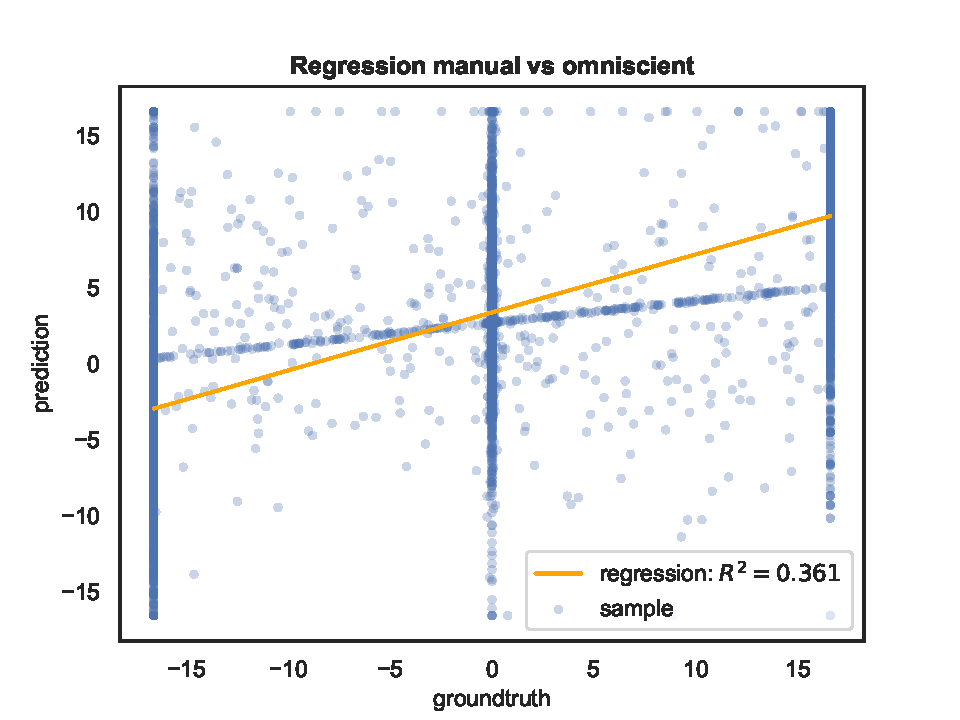
\includegraphics[width=\textwidth]{contents/images/net-d6/regression-manualvsomniscient}%
	\end{subfigure}
	\hfill
	\begin{subfigure}[h]{0.49\textwidth}
		\centering
		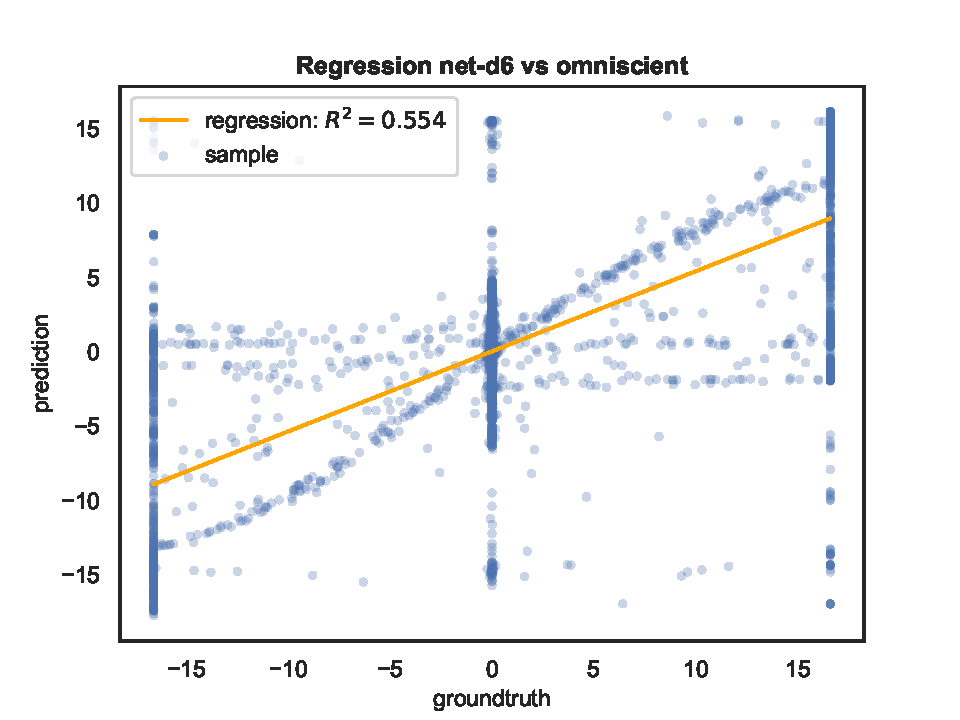
\includegraphics[width=\textwidth]{contents/images/net-d6/regression-net-d6-vs-omniscient}
	\end{subfigure}
	\caption[Evaluation of the \gls{r2} coefficients of \texttt{net-d6} .]{Comparison 
	of the \gls{r2} coefficient of the manual and the controller learned from 
	\texttt{net-d6} with respect to the omniscient one.}
	\label{fig:net-d6r2}
\end{figure}

Moreover, as shown in Figure \ref{fig:net-d6r2}, we expect that the robots’ 
behaviour using the learned instead of the manual controller is better, even if far 
from the expert.

In Figure \ref{fig:net-d6traj} are shown the trajectories obtained employing the 
three controllers. 
\begin{figure}[!htb]
	\begin{center}
		\begin{subfigure}[h]{0.49\textwidth}
			\centering
			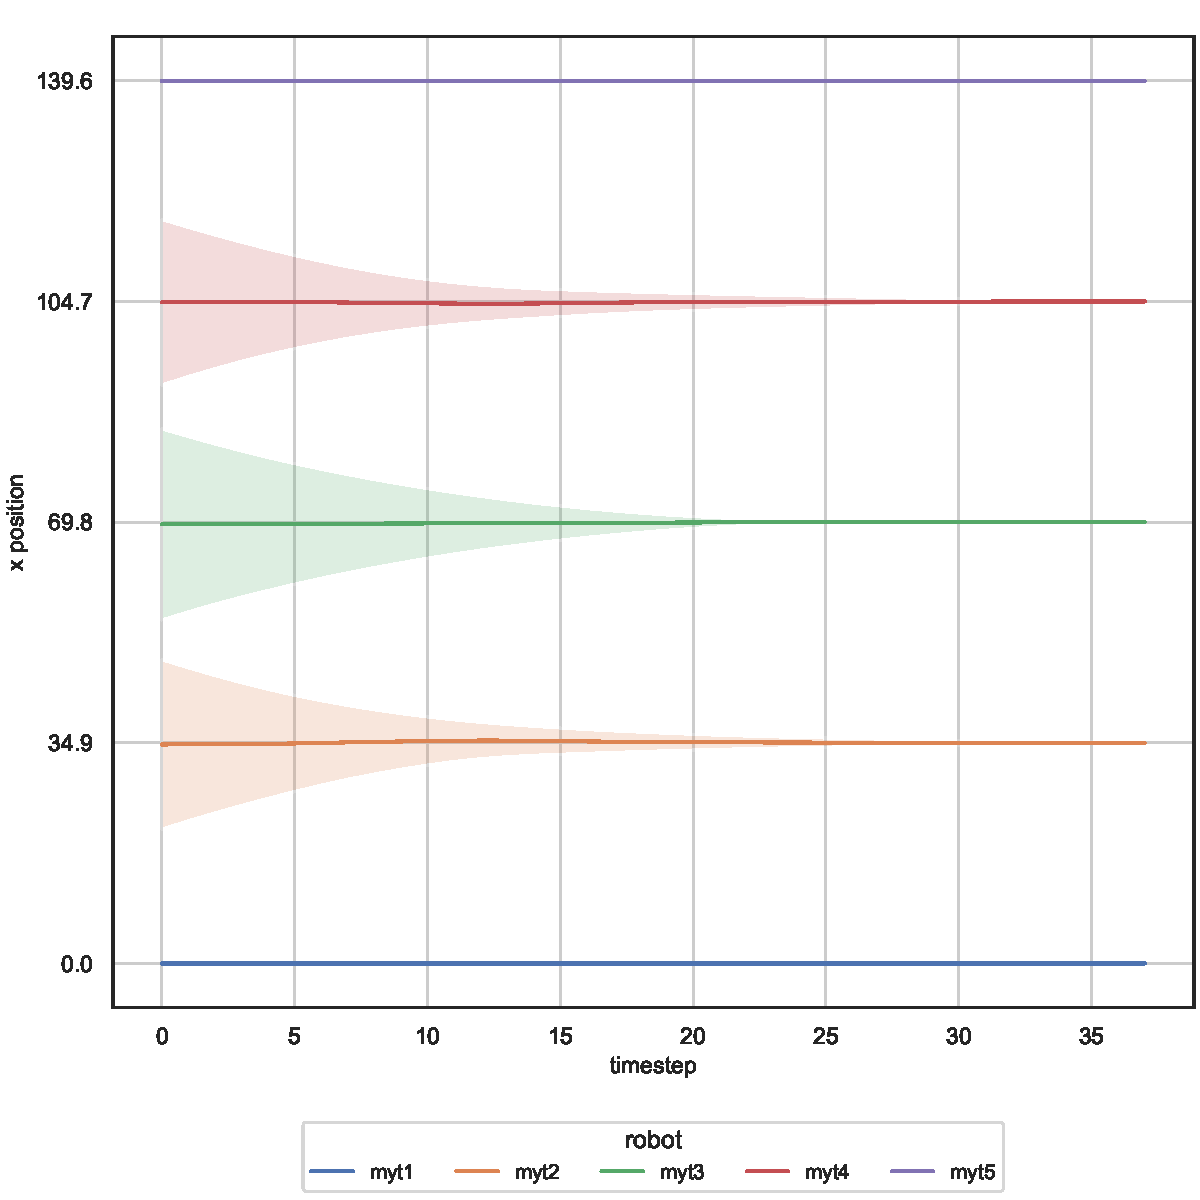
\includegraphics[width=.95\textwidth]{contents/images/net-d6/position-overtime-omniscient}%
			\caption{Expert controller trajectories.}
		\end{subfigure}
		\hfill
		\begin{subfigure}[h]{0.49\textwidth}
			\centering
			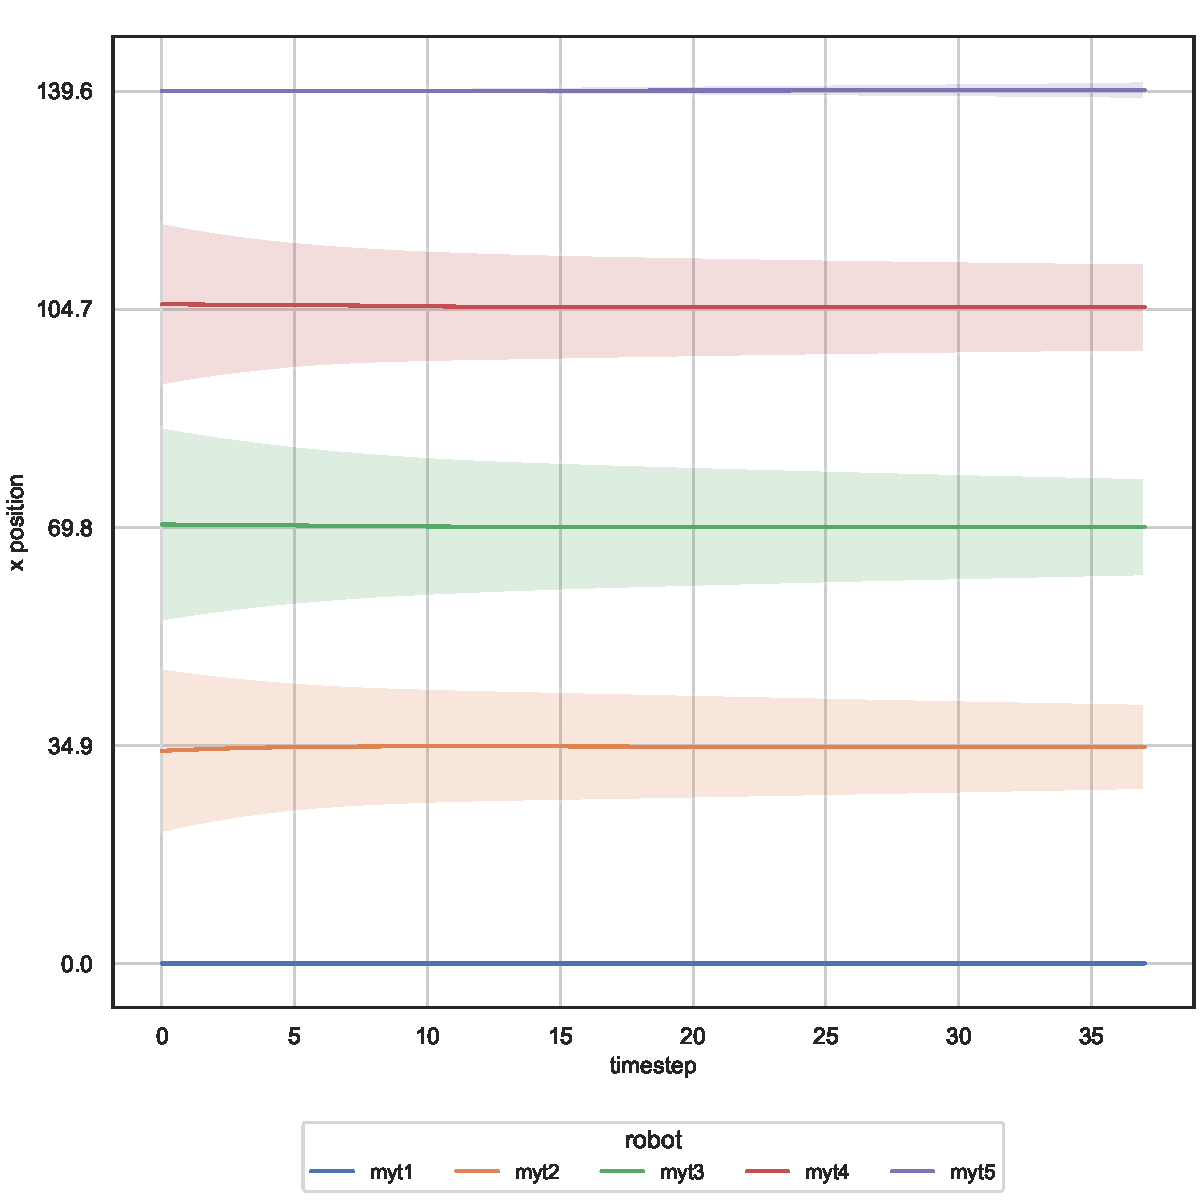
\includegraphics[width=.95\textwidth]{contents/images/net-d6/position-overtime-learned_distributed}
			\caption{Distributed controller trajectories.}
		\end{subfigure}
	\end{center}
	\begin{center}
	\begin{subfigure}[h]{0.49\textwidth}
		\centering			
		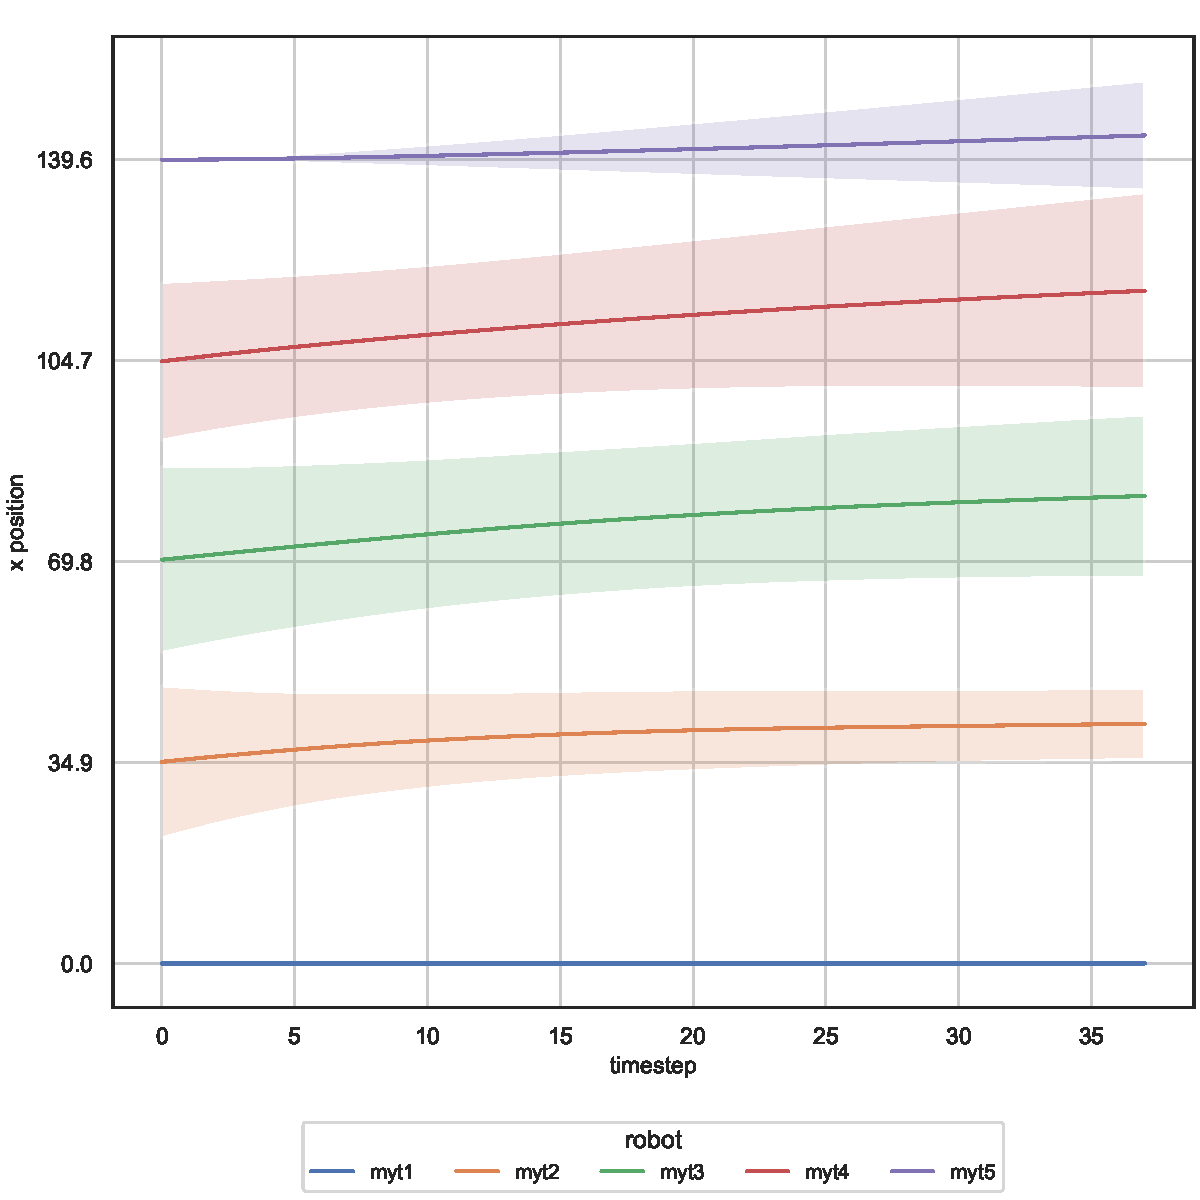
\includegraphics[width=.95\textwidth]{contents/images/net-d6/position-overtime-manual}%
		\caption{Manual controller trajectories.}
	\end{subfigure}
	\hfill
	\begin{subfigure}[h]{0.49\textwidth}
		\centering
		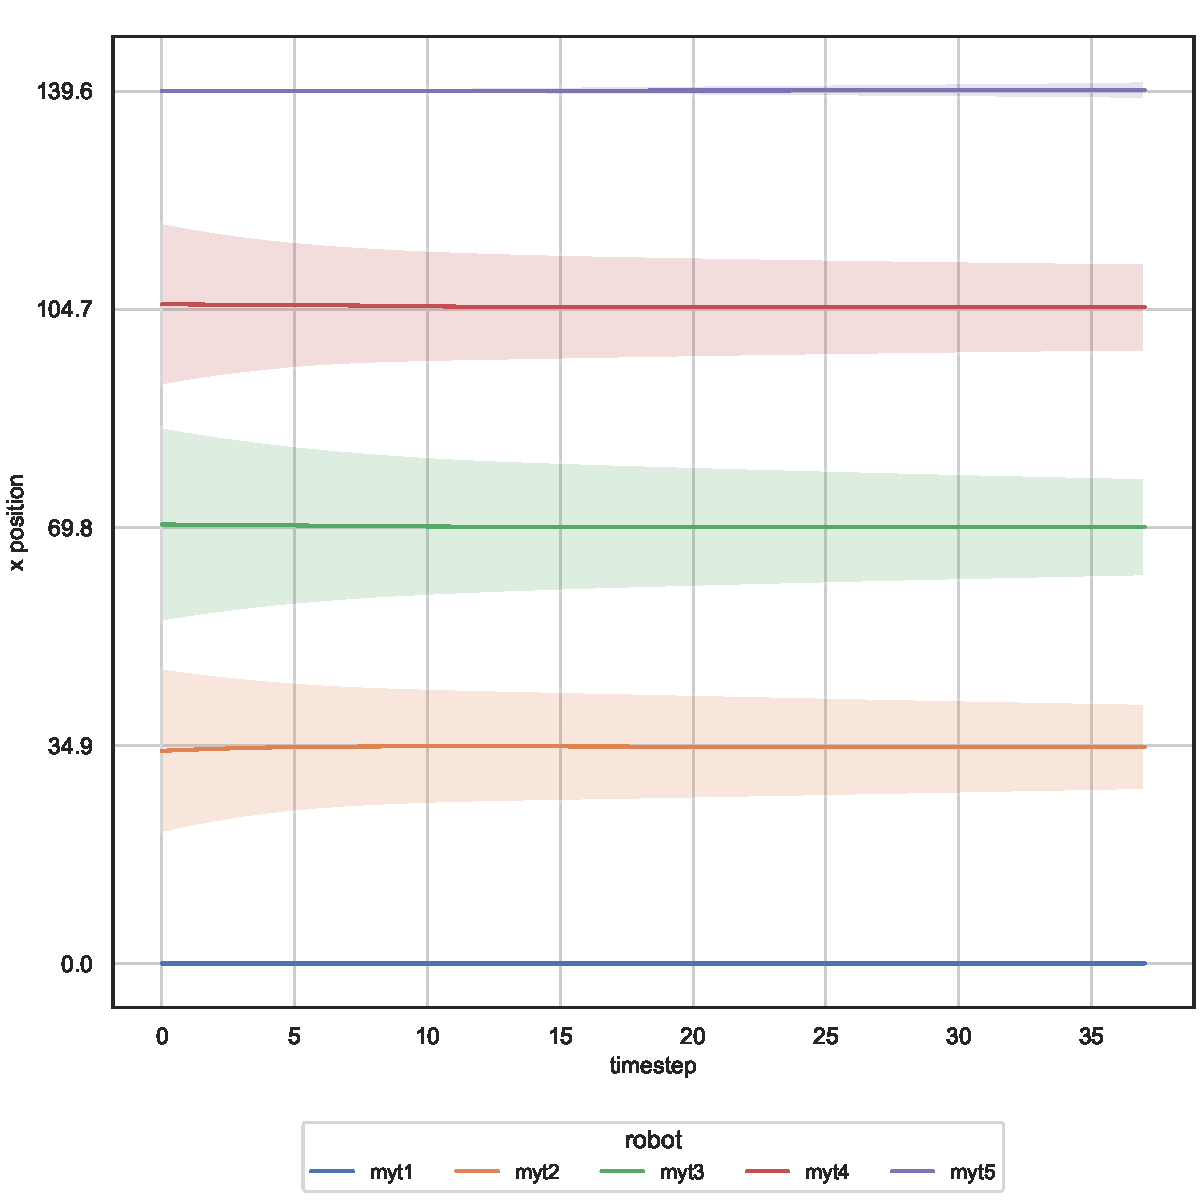
\includegraphics[width=.95\textwidth]{contents/images/net-d6/position-overtime-learned_distributed}
		\caption{Distributed controller trajectories.}
	\end{subfigure}
	\end{center}
	\caption[Evaluation of the trajectories learned by \texttt{net-d6}.]{Comparison 
	of trajectories generated using three controllers: the expert, the manual and 
	the one learned from \texttt{net-d6}.}
	\label{fig:net-d6traj}
\end{figure}
As before, the robot positions are averaged over all the runs. 
Even for the expert, the convergence to the target is slower than before, 
as expected since the distance between the robots is greater, but it is much faster 
than with the other two controllers.
The manual controller has serious problems in reaching the goal: even if the 
agents try to position themselves at equal distances, they tend to increase the 
average gap between them, creating situations in which the last robot in motion 
hits the fixed one. 
Surprisingly, the learned controller allows the agents to converge to the correct 
configuration by taking more time than the expert does.

An immediate examination of the evolution of the control over time, in Figure 
\ref{fig:net-d6control}, highlights the speed of the expert controller, which in all 
the simulation runs after $25$ time steps has reached the goal. 
In addition, the manual controller always sets a positive speed, which leads to the 
wrong behaviour mentioned earlier, while the slowness of the distributed 
control is explained by the use of a low speed.
\begin{figure}[!htb]
	\centering
	\begin{subfigure}[h]{0.3\textwidth}
		\centering
		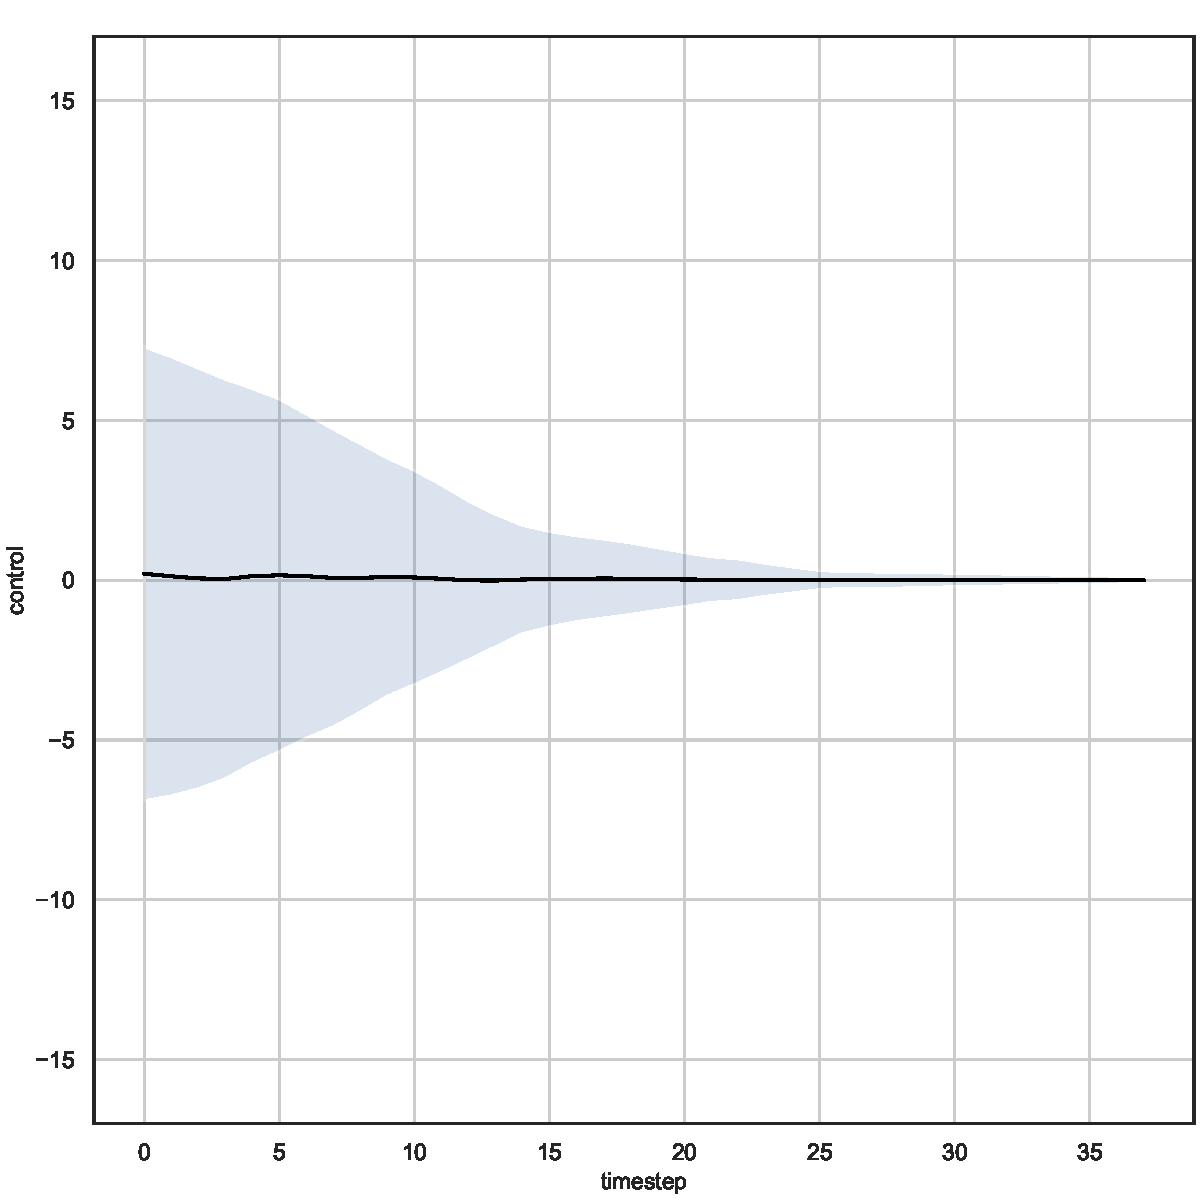
\includegraphics[width=\textwidth]{contents/images/net-d6/control-overtime-omniscient}%
		\caption{Expert controller.}
	\end{subfigure}
	\hfill
	\begin{subfigure}[h]{0.3\textwidth}
		\centering
		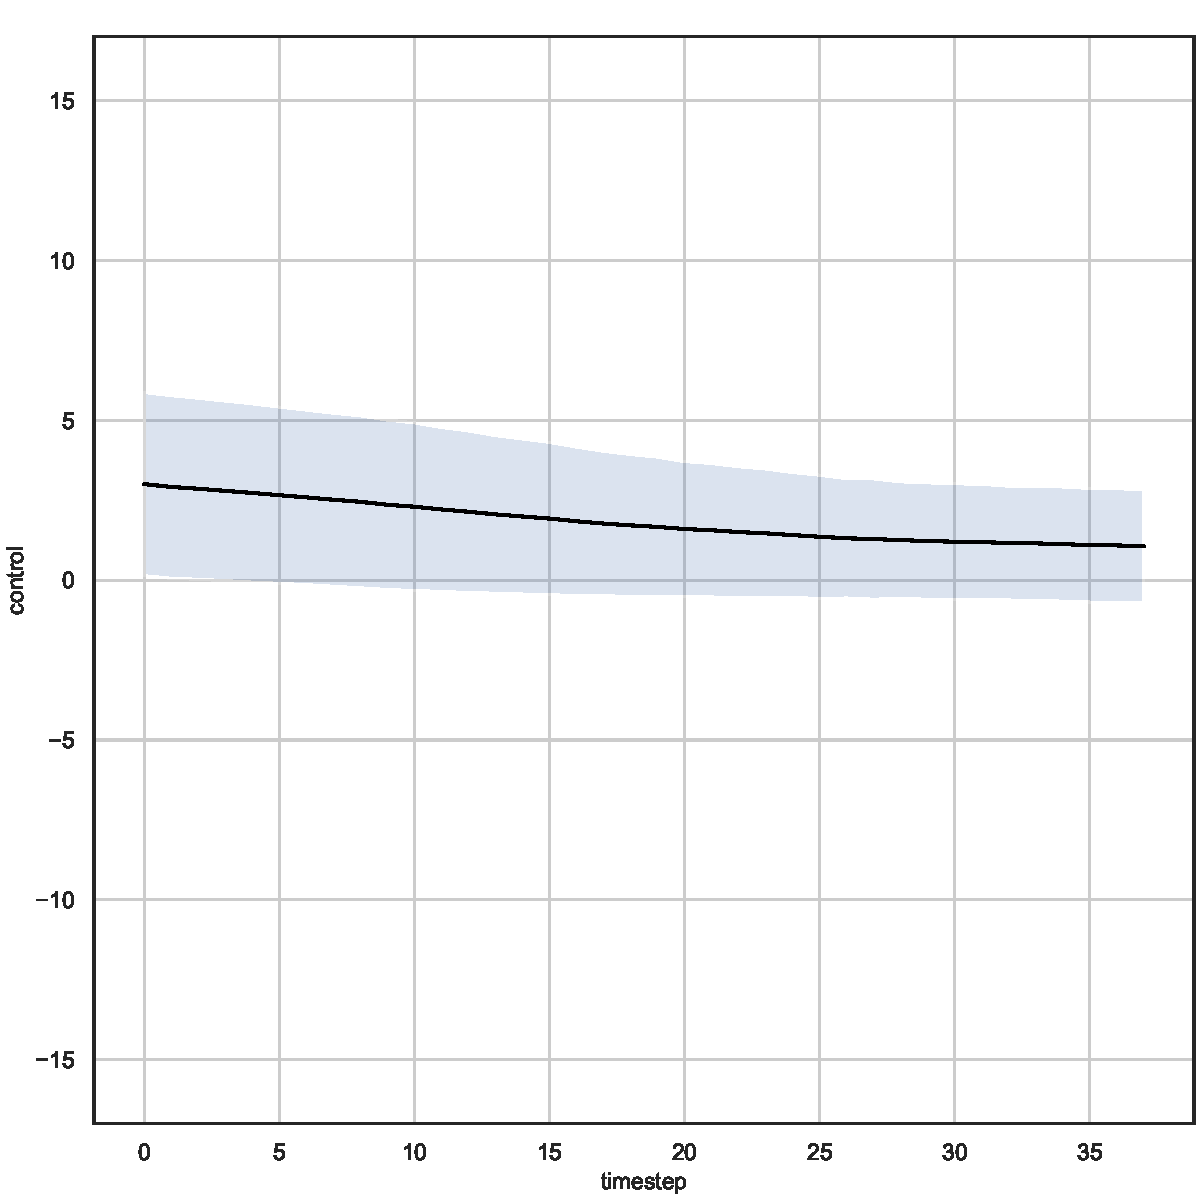
\includegraphics[width=\textwidth]{contents/images/net-d6/control-overtime-manual}%
		\caption{Manual controller.}
	\end{subfigure}
	\hfill
	\begin{subfigure}[h]{0.3\textwidth}
		\centering
		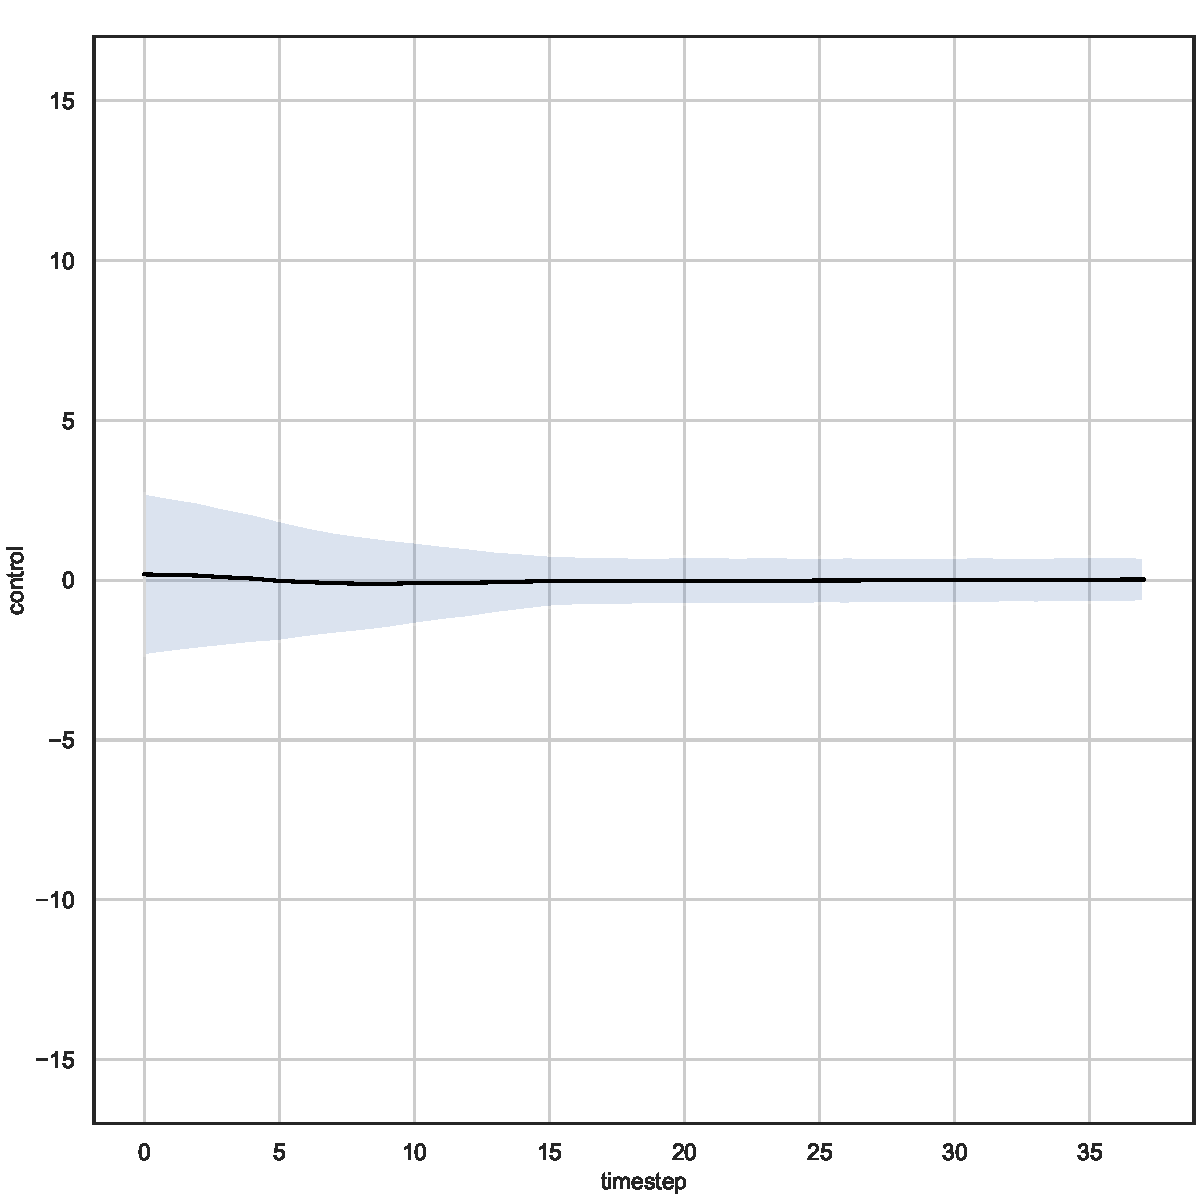
\includegraphics[width=\textwidth]{contents/images/net-d6/control-overtime-learned_distributed}
		\caption{Distributed controller.}
	\end{subfigure}
	\caption[Evaluation of the control decided by \texttt{net-d6}.]{Comparison 
		of output control decided using three controllers: the expert, the manual 
		and the one learned from \texttt{net-d6}.}
	\label{fig:net-d6control}
\end{figure}

Figure \ref{fig:net-d6responsesensors} visualises the response of the learned 
controller as the input sensing changes, analysing the same two cases as before. 
Despite the behaviour is the same obtained using \texttt{prox\_values} when the 
robot sees only behind, this time the trend is different when the robot sees 
nothing behind: since the robot has to move backwards, a negative speed is 
always returned, that is higher when the obstacle is far. 
\begin{figure}[!htb]
	\centering
	\begin{subfigure}[h]{0.49\textwidth}
		\centering
		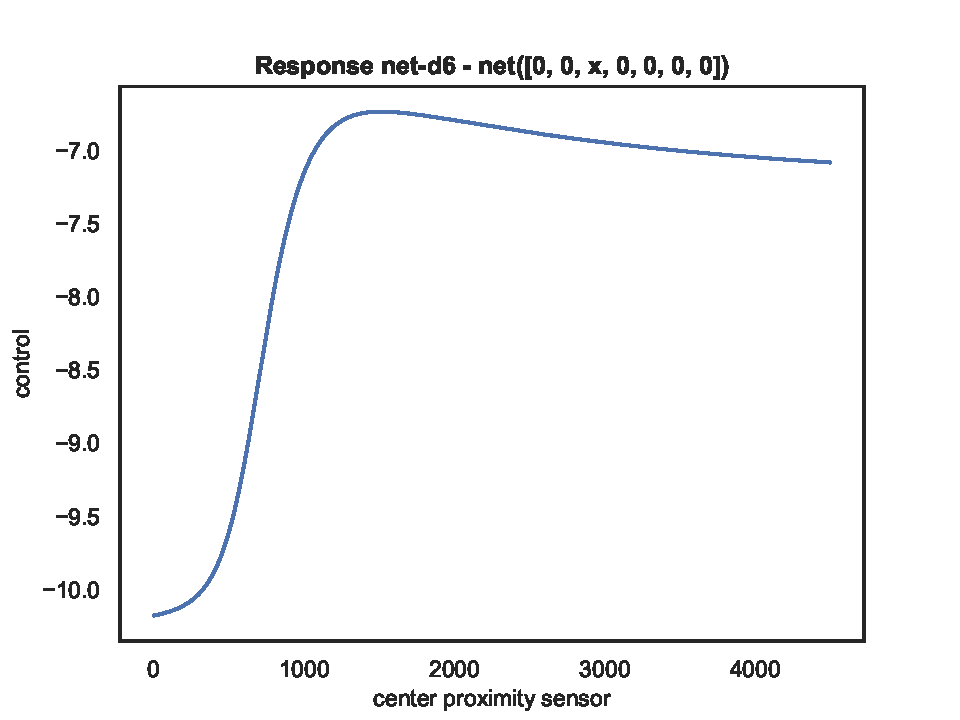
\includegraphics[width=\textwidth]{contents/images/net-d6/response-net-d6-front}%
	\end{subfigure}
	\hfill
	\begin{subfigure}[h]{0.49\textwidth}
		\centering
		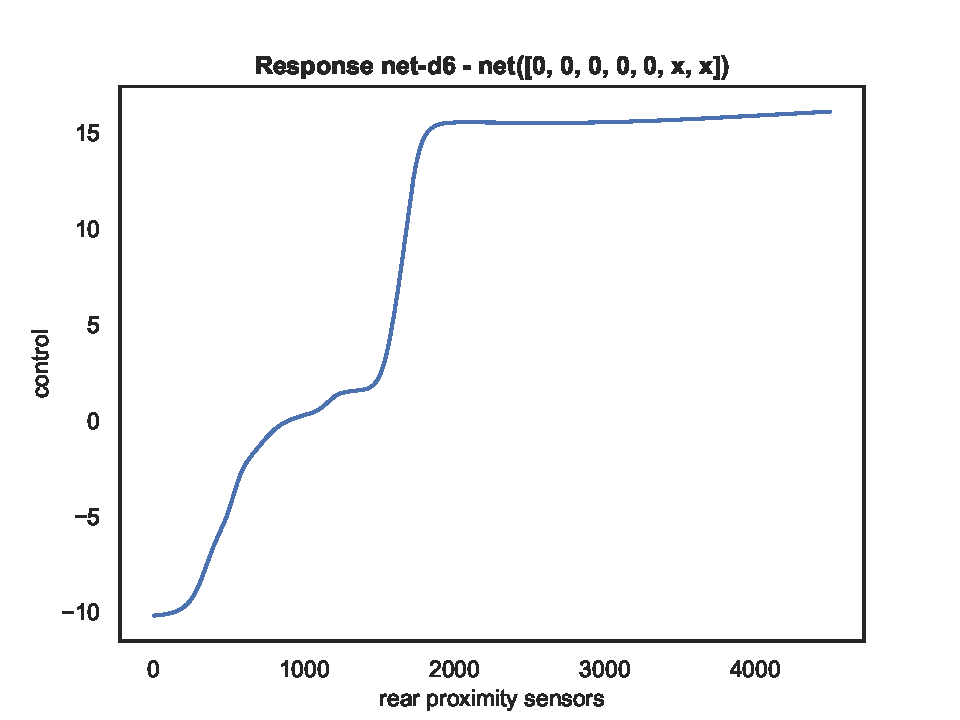
\includegraphics[width=\textwidth]{contents/images/net-d6/response-net-d6-rear}
	\end{subfigure}
	\caption{Response of \texttt{net-d6} by varying the input sensing.}
	\label{fig:net-d6responsesensors}
\end{figure}

In Figure \ref{fig:net-d6responseposition} is displayed the behaviour of a robot 
located between two that are already in their place.
\begin{figure}[!htb]
	\centering
	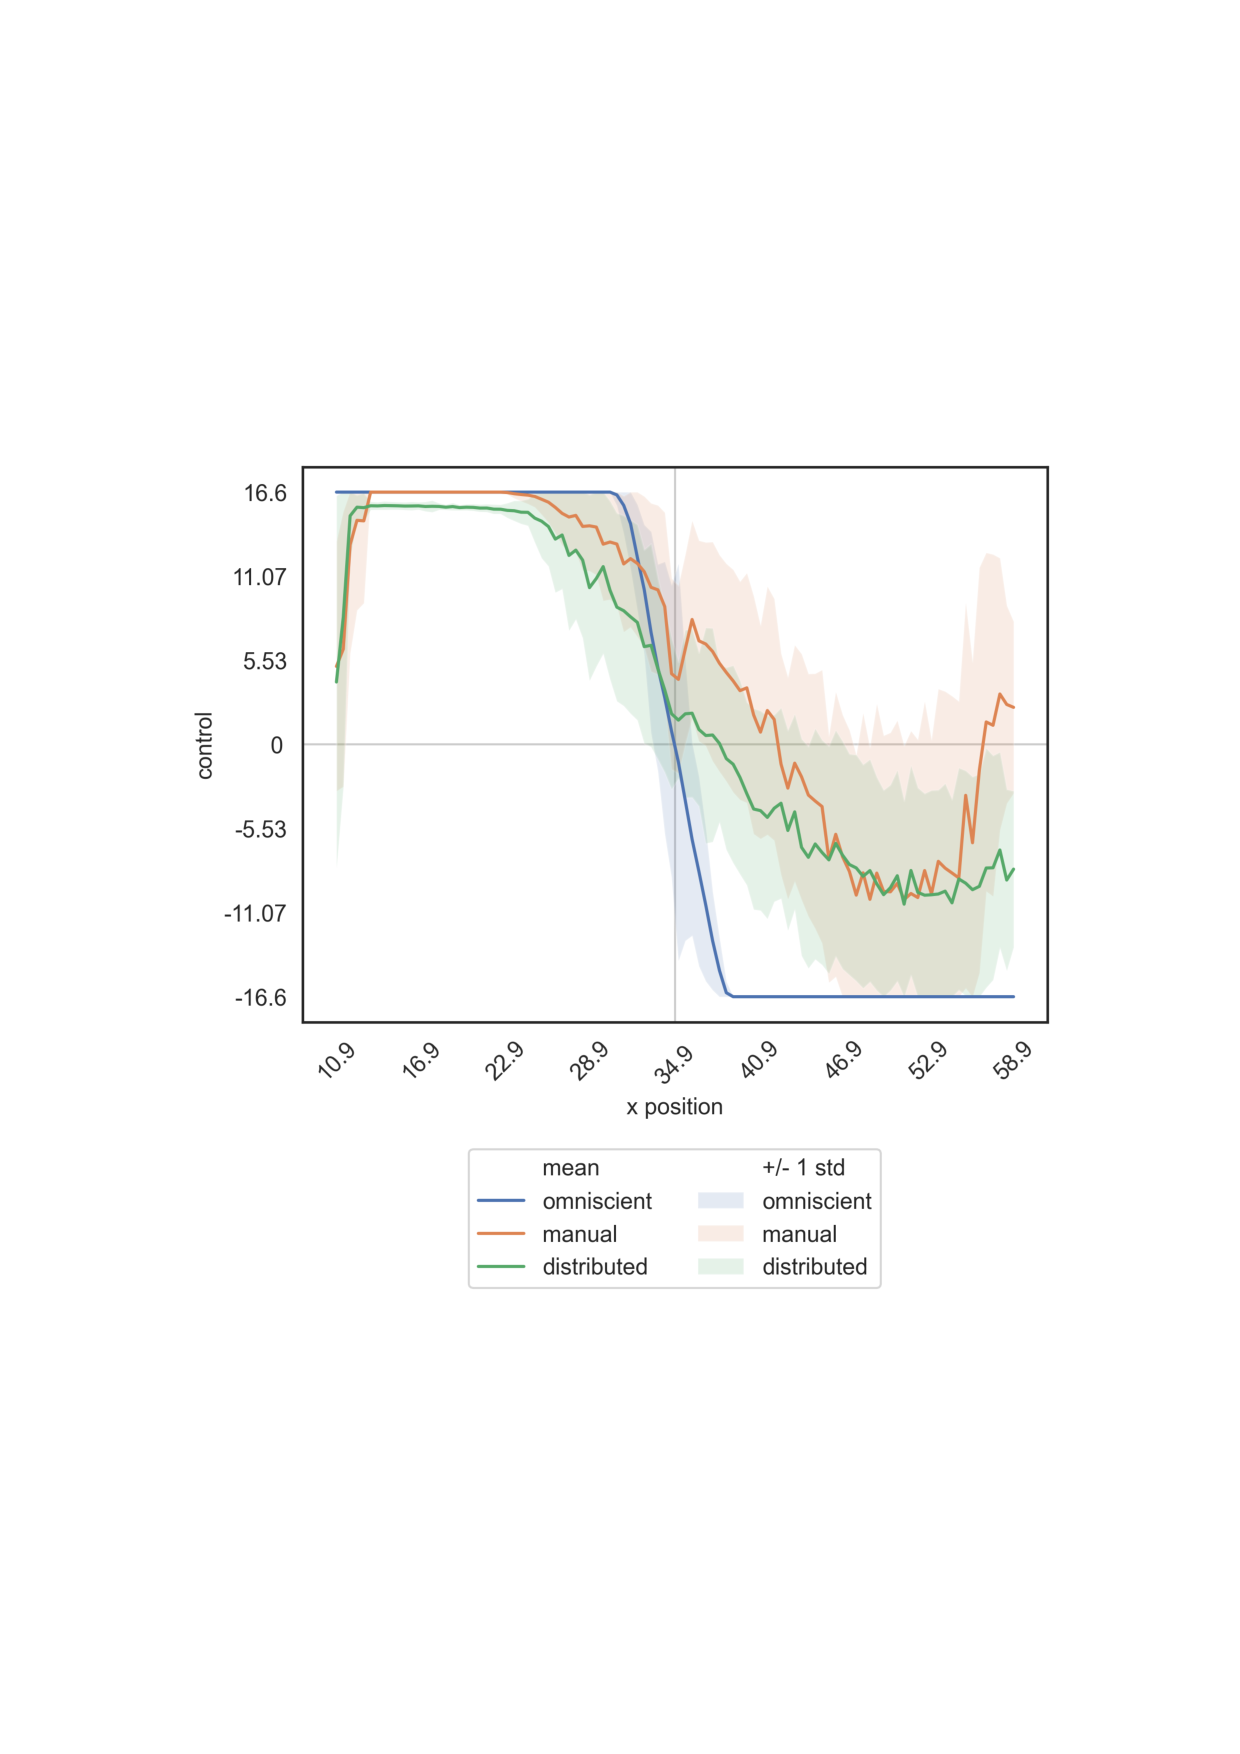
\includegraphics[width=.45\textwidth]{contents/images/net-d6/response-varying_init_position-distributed}%
	\caption{Response of \texttt{net-d6} by varying the initial position.}
	\label{fig:net-d6responseposition}
\end{figure}
It visualises the response of the learned controller by varying the distance 
between two stationary agents and a robot located among them.
As expected, the output is a high positive value when the robot is close to an 
obstacle on the left, it decreases and reaches $0$ when the distance from 
right and left is equal, and finally becomes negative when there is an obstacle in 
front and not behind. 

Finally, in Figure \ref{fig:net-d6distance} is presented the average distance of the 
robots from the target among all the simulations. 
\begin{figure}[!htb]
	\centering
	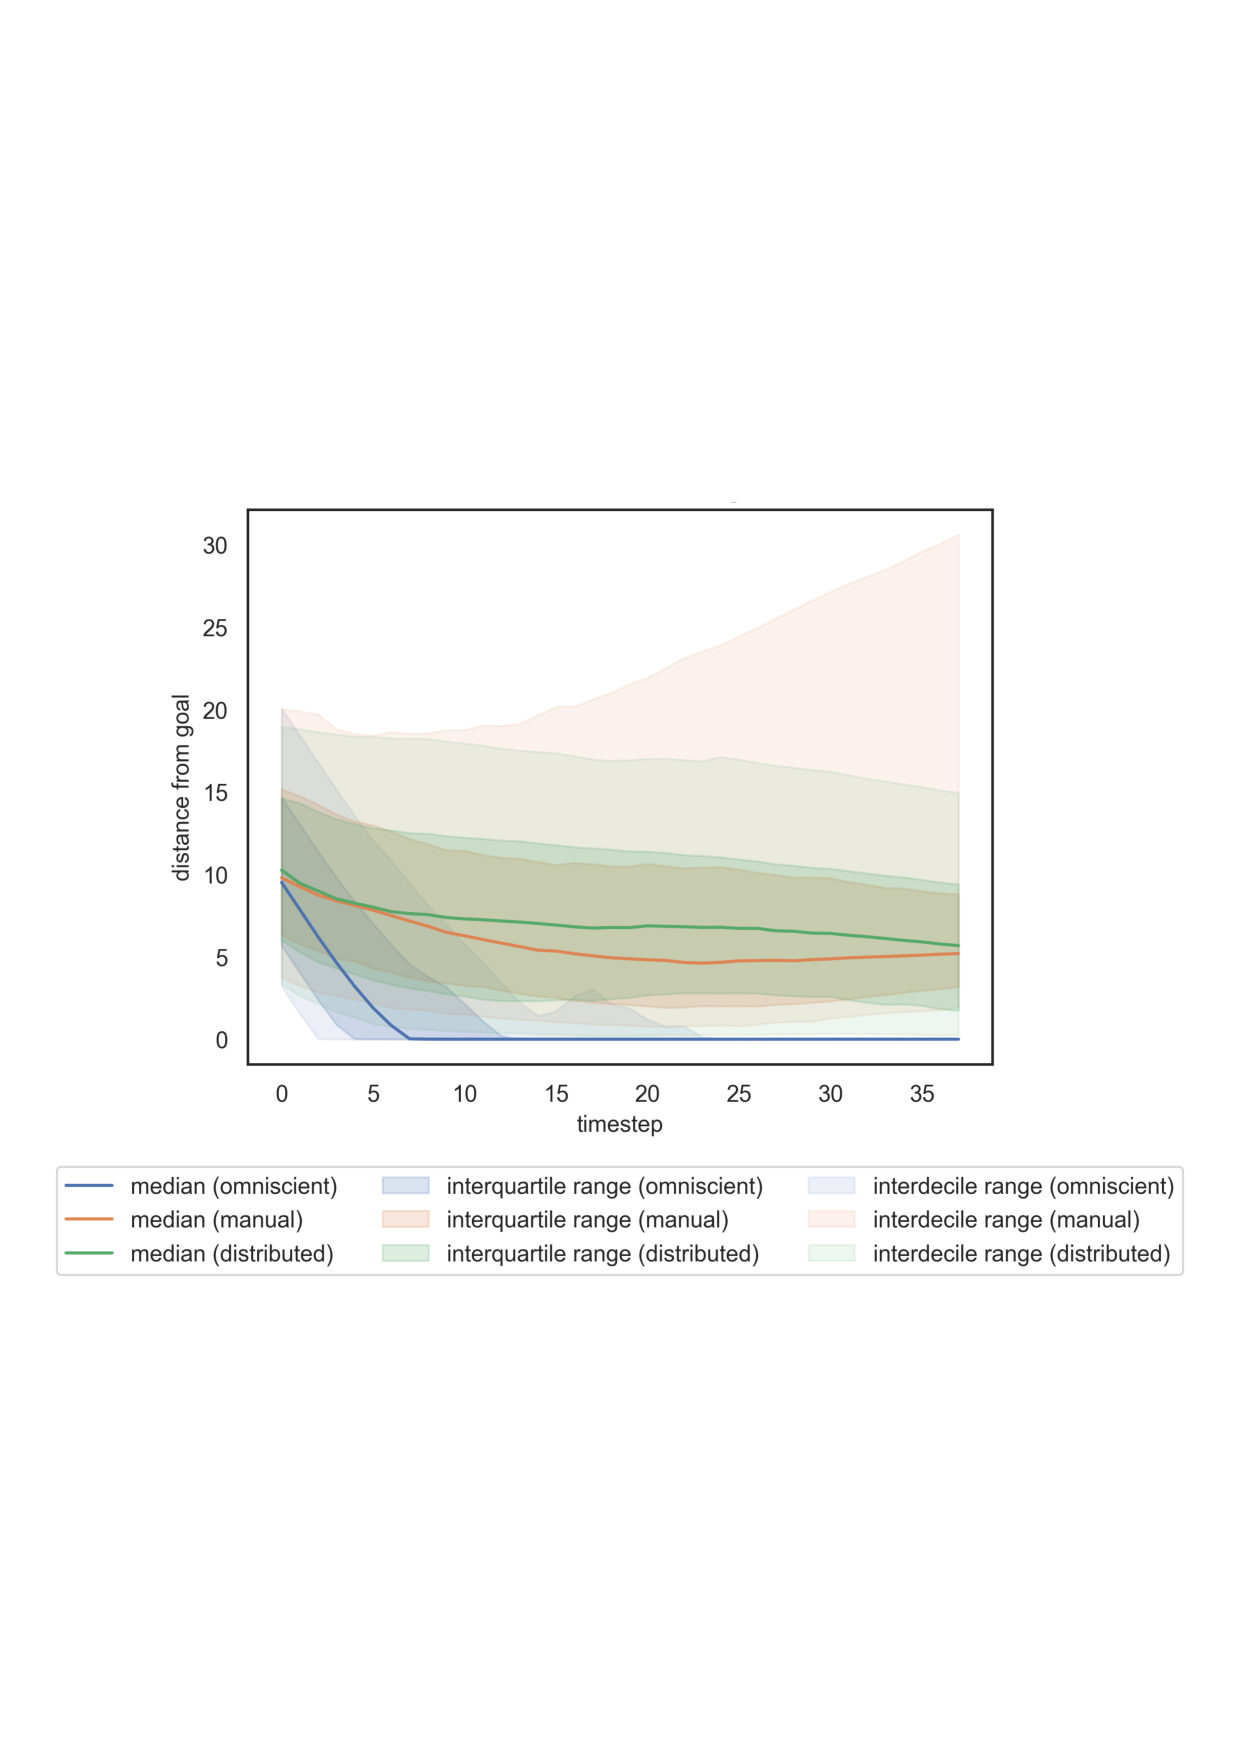
\includegraphics[width=.65\textwidth]{contents/images/net-d6/distances-from-goal-compressed-distributed}%
		\caption[Evaluation of \texttt{net-d6} distances from goal.]{Comparison of 
		performance in terms of distances from goal obtained using three 
		controllers: the expert, the manual and the one learned from \texttt{net-d6}.}
	\label{fig:net-d6distance}
\end{figure}
The performance of the learned and the manual controllers are similar: in the 
final configuration they both are at about $5$\gls{cm} from the target. 

We conclude the first group of experiments presenting the results obtained 
using both types of input together from which we expect a more stable and 
robust behaviour. 
In Figure \ref{fig:distlossall} an analysis of the losses shows that using 
\texttt{all\_sensors} inputs the network is able to work well with all the 
gaps. 
\begin{figure}[!htb]
	\centering
	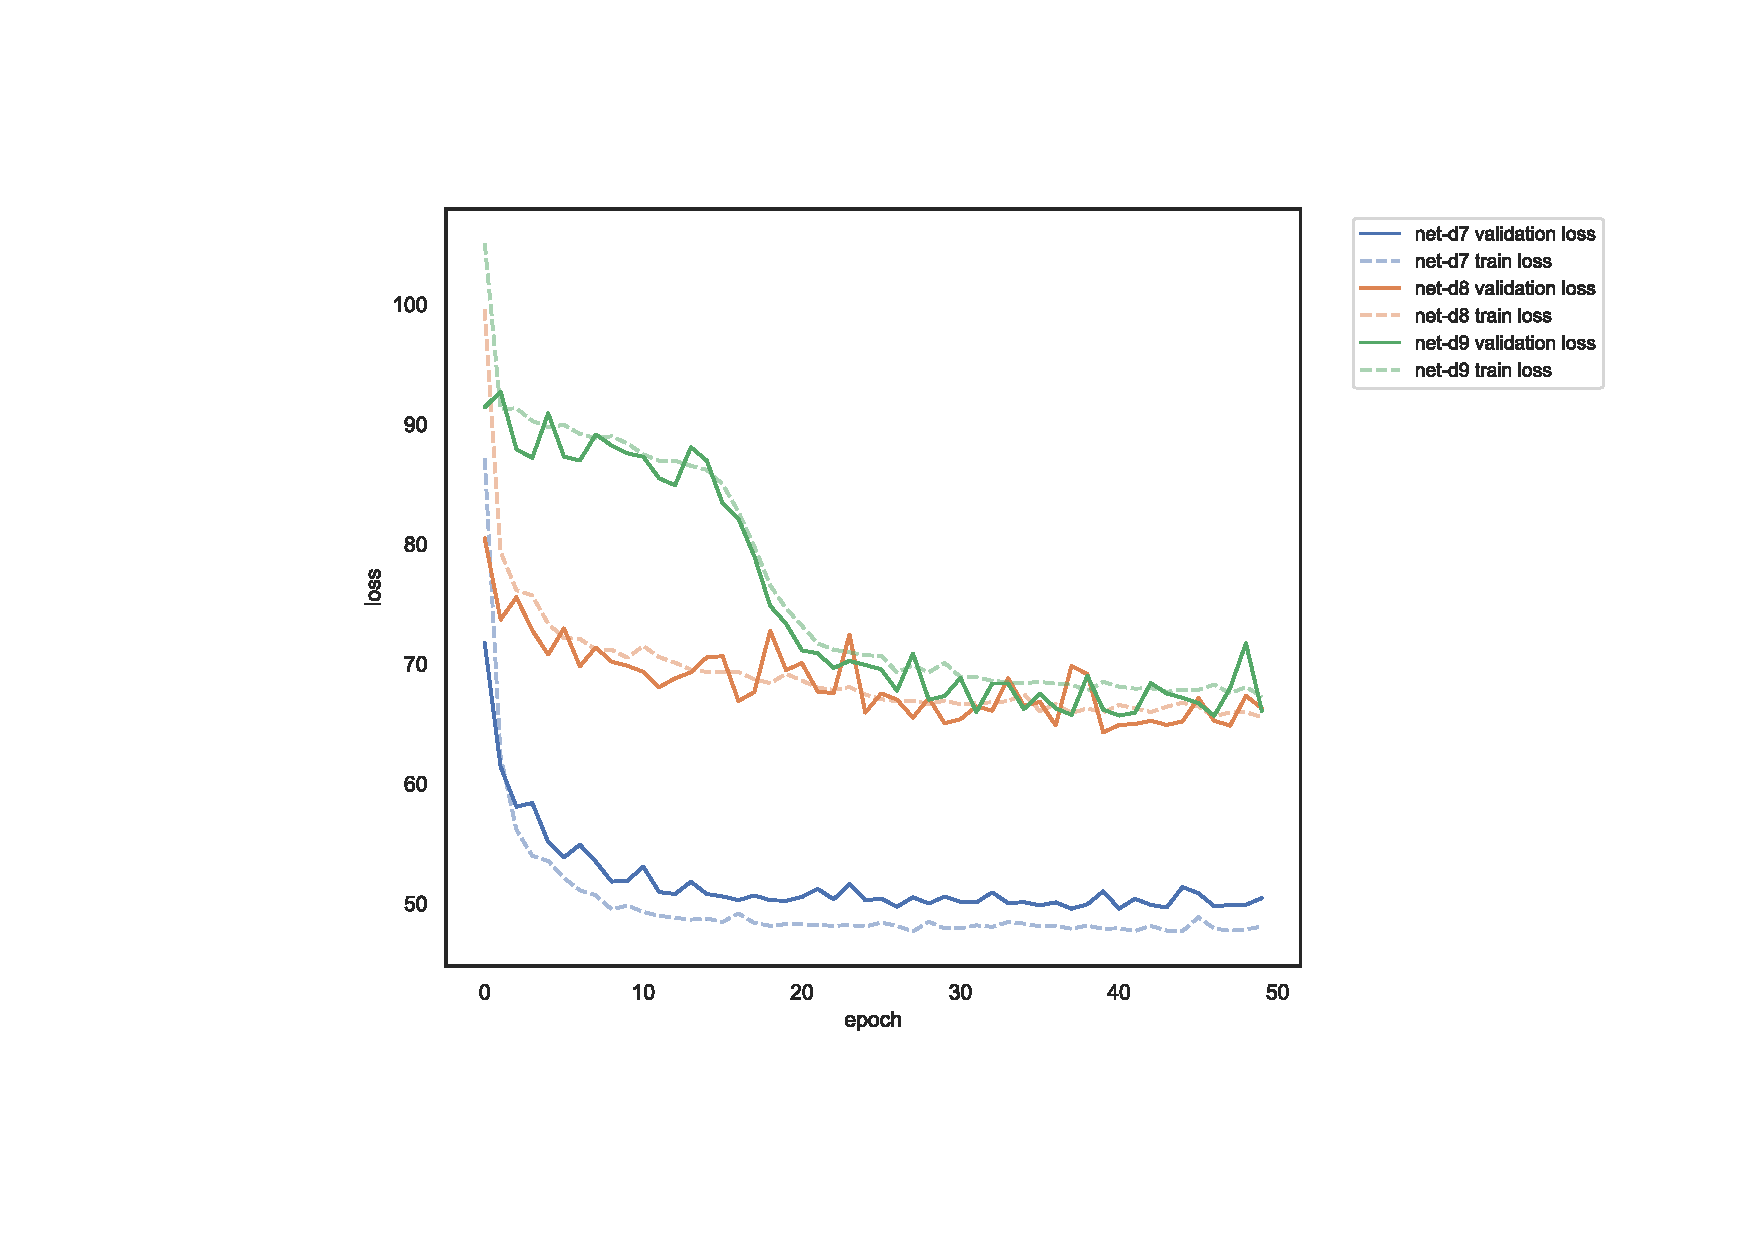
\includegraphics[width=.8\textwidth]{contents/images/task1/loss-distributed-all_sensors@}%
	\caption{Comparison of the losses of the models that use \texttt{all\_sensors} 
		readings.}
	\label{fig:distlossall}
\end{figure}

Examining the \gls{r2} coefficients in Figure \ref{fig:net-d789r2}, the behaviour 
obtained with \texttt{net-d7} and \texttt{net-d9} are the more promising. 
\begin{figure}[!htb]
	\begin{center}
		\begin{subfigure}[h]{0.49\textwidth}
 			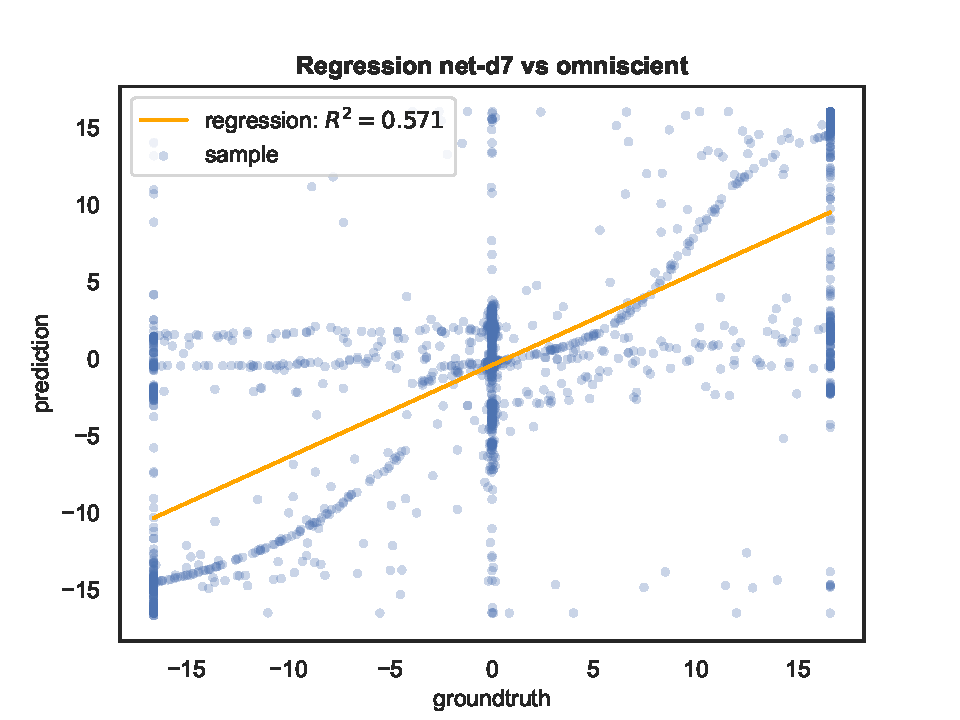
\includegraphics[width=\textwidth]{contents/images/net-d7/regression-net-d7-vs-omniscient}%
		\end{subfigure}
		\hfill
		\begin{subfigure}[h]{0.49\textwidth}
			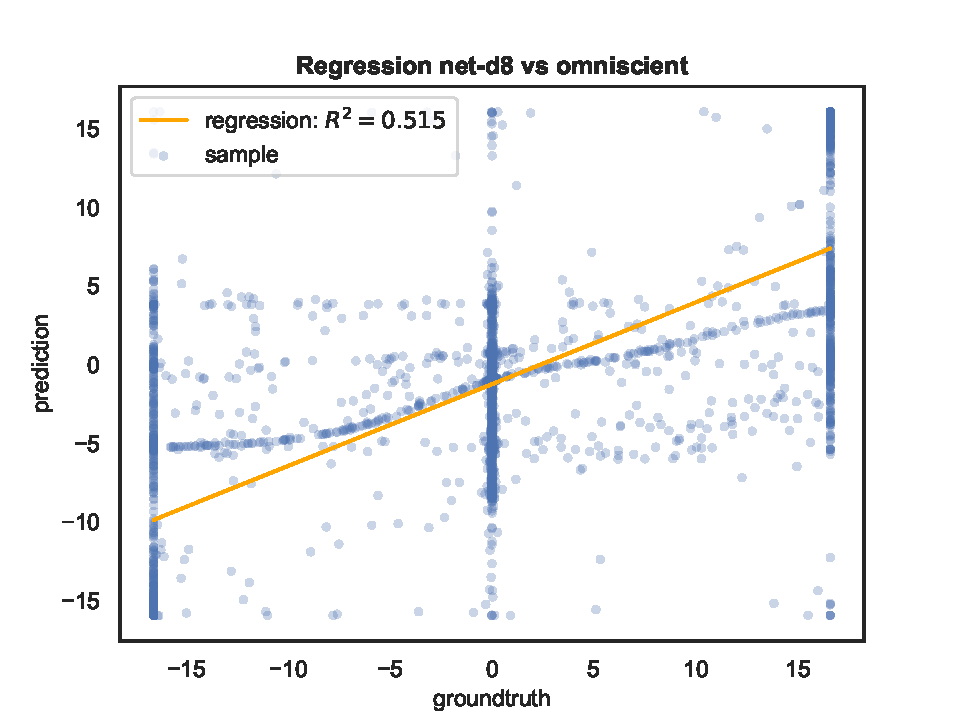
\includegraphics[width=\textwidth]{contents/images/net-d8/regression-net-d8-vs-omniscient}%
		\end{subfigure}
	\end{center}
	\hfil\vspace{-0.8cm}
	\begin{center}
		\begin{subfigure}[h]{0.49\textwidth}
			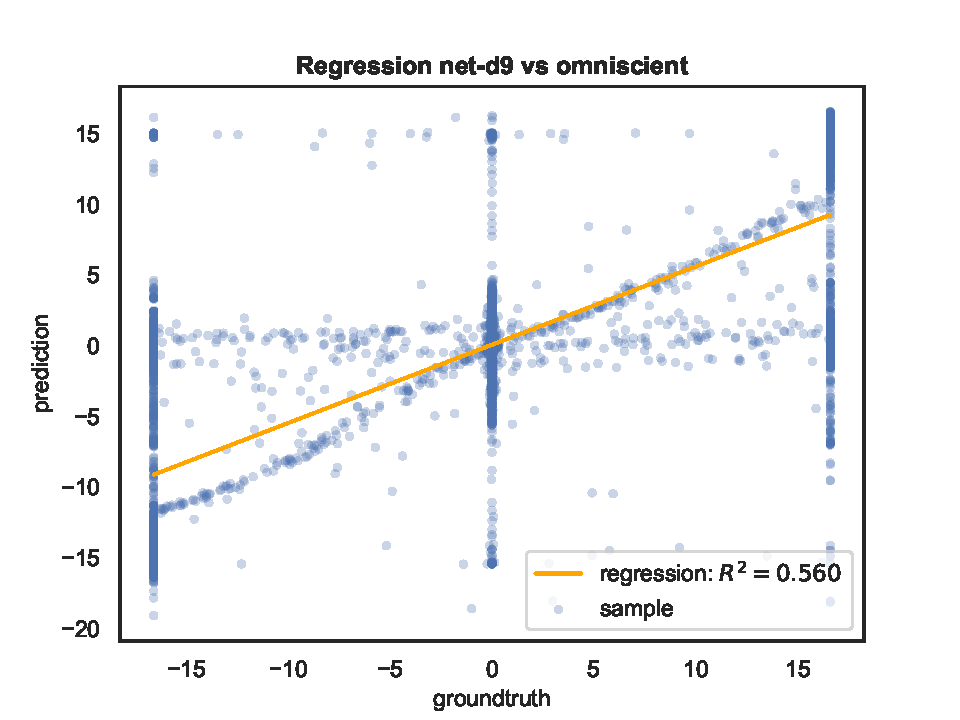
\includegraphics[width=\textwidth]{contents/images/net-d9/regression-net-d9-vs-omniscient}
		\end{subfigure}
	\end{center}
	\caption[Comparison of the \gls{r2} coefficients for \texttt{prox\_comm} 
	readings.]{Comparison of the \gls{r2} coefficients of the models that use 
		\texttt{prox\_comm} readings.}
	\label{fig:net-d789r2}
\end{figure}

\bigskip
Considering the more complex case, that is the one with the greatest average gap,
the superiority of this controller is further supported by the comparisons in Figure
\ref{fig:net-d9r2}. 
\begin{figure}[!htb]
	\centering
	\begin{subfigure}[h]{0.49\textwidth}
		\centering
		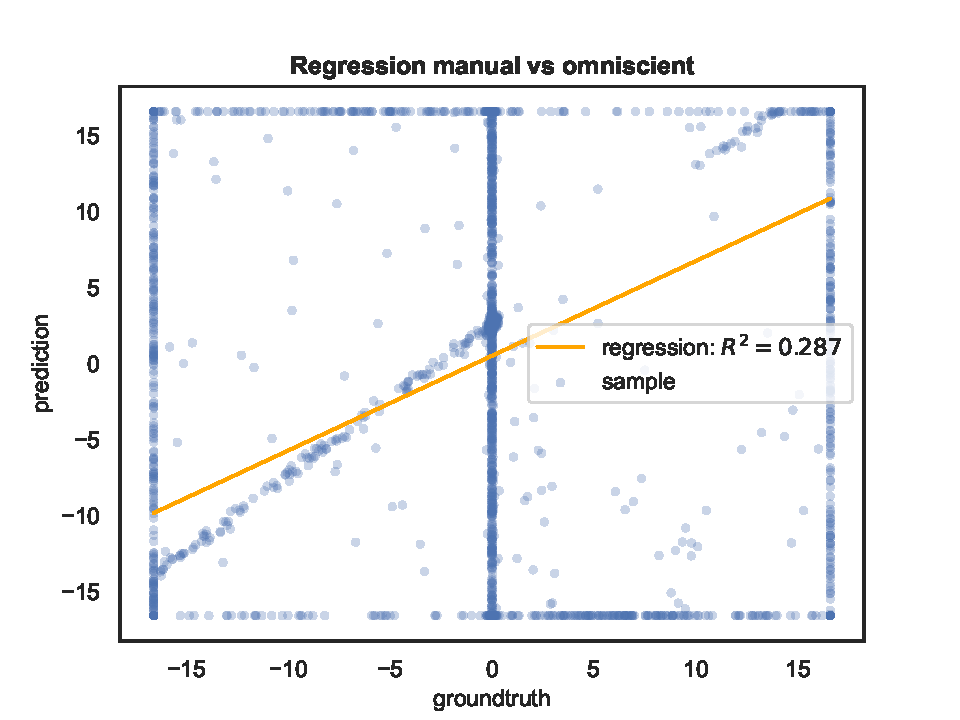
\includegraphics[width=\textwidth]{contents/images/net-d9/regression-manualvsomniscient}%
	\end{subfigure}
	\hfill
	\begin{subfigure}[h]{0.49\textwidth}
		\centering
		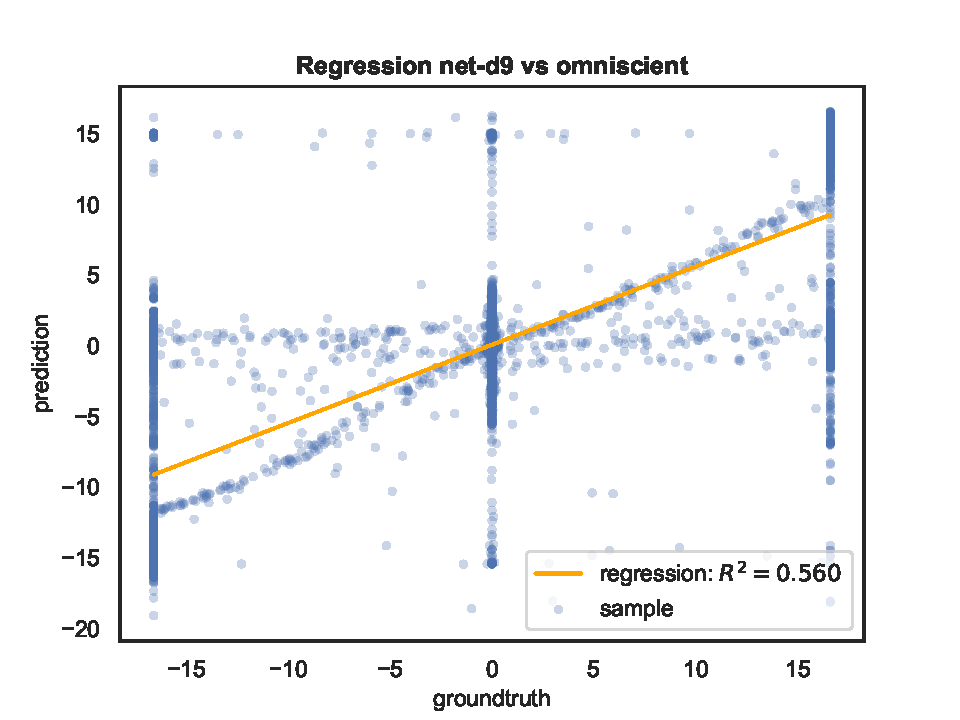
\includegraphics[width=\textwidth]{contents/images/net-d9/regression-net-d9-vs-omniscient}
	\end{subfigure}
	\caption[Evaluation of the \gls{r2} coefficients of \texttt{net-d9}.]{Comparison 
	of the \gls{r2} coefficient of the manual and the controller learned from 
	\texttt{net-d9} with respect to the omniscient one.}
	\label{fig:net-d9r2}
\end{figure}

In Figure \ref{fig:net-d9traj} are shown trajectories obtained employing the three 
controllers. The convergence to the target is still slow, even if this time the expert 
need less time steps than before. 
The manual controller does not shows the same problem has before, while the 
learned controller is still the slowest to end up in the correct configuration.

Examining the evolution of the output control, in Figure \ref{fig:net-d9control}, 
the plots of the expert and the learned controller are similar, although the speed 
in the second is much lower.

In Figure \ref{fig:net-d9responseposition} is displayed the behaviour of a robot 
located between two that are already in their place.
This time the trend of the three curves shows how the behaviour of the model 
learned and of the manual controller are similar to that of the expert.

\begin{figure}[!htb]
	\begin{center}
		\begin{subfigure}[h]{0.49\textwidth}
			\centering
			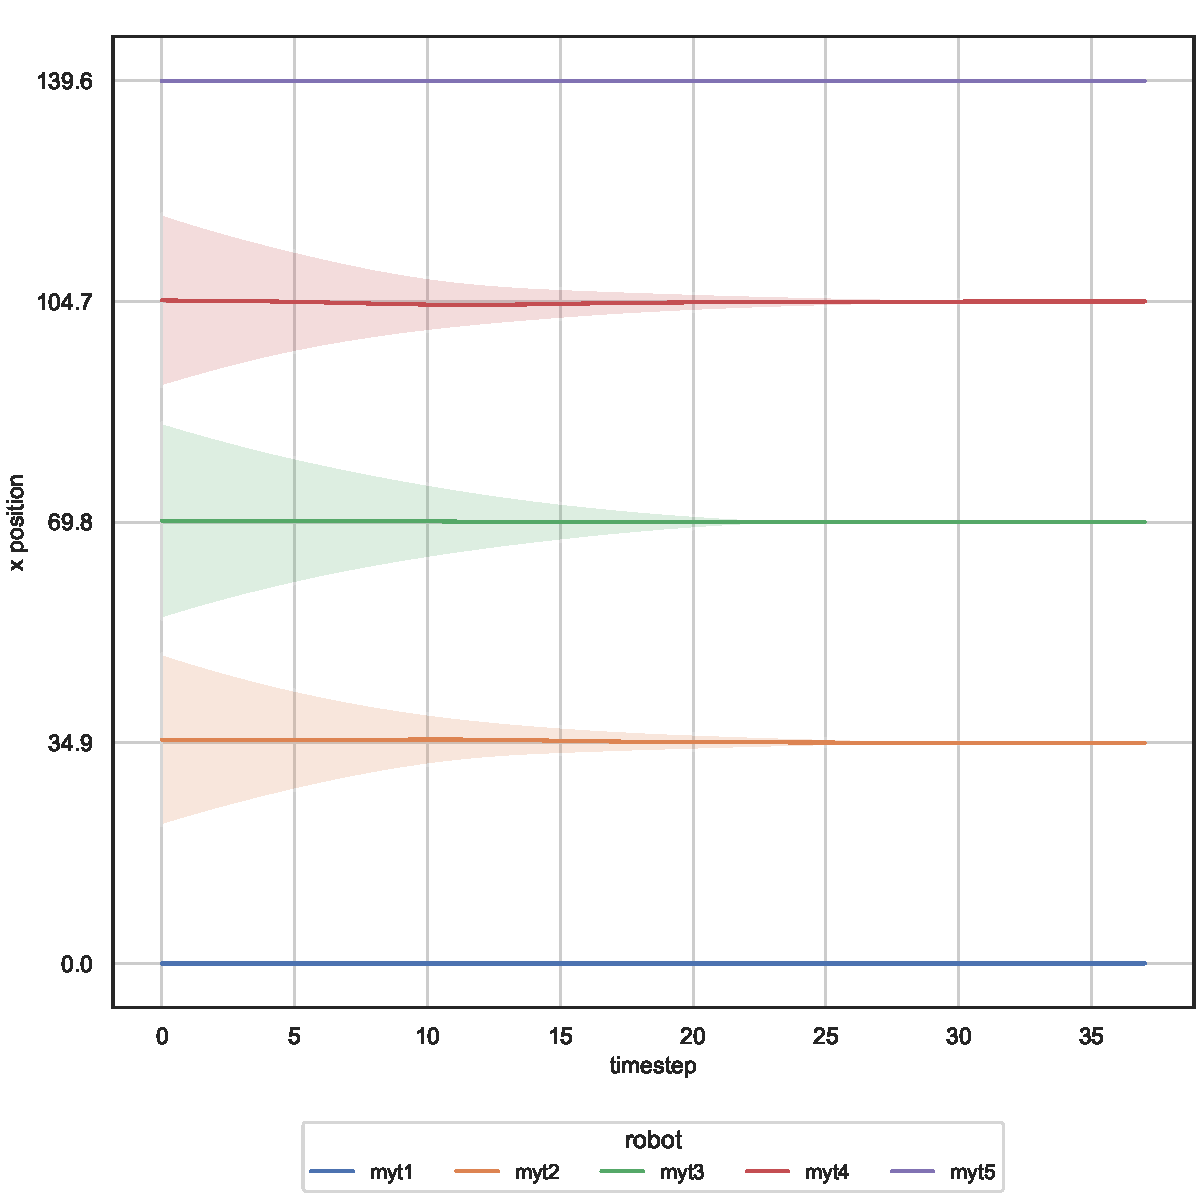
\includegraphics[width=.95\textwidth]{contents/images/net-d9/position-overtime-omniscient}%
			\caption{Expert controller trajectories.}
		\end{subfigure}
		\hfill
		\begin{subfigure}[h]{0.49\textwidth}
			\centering
			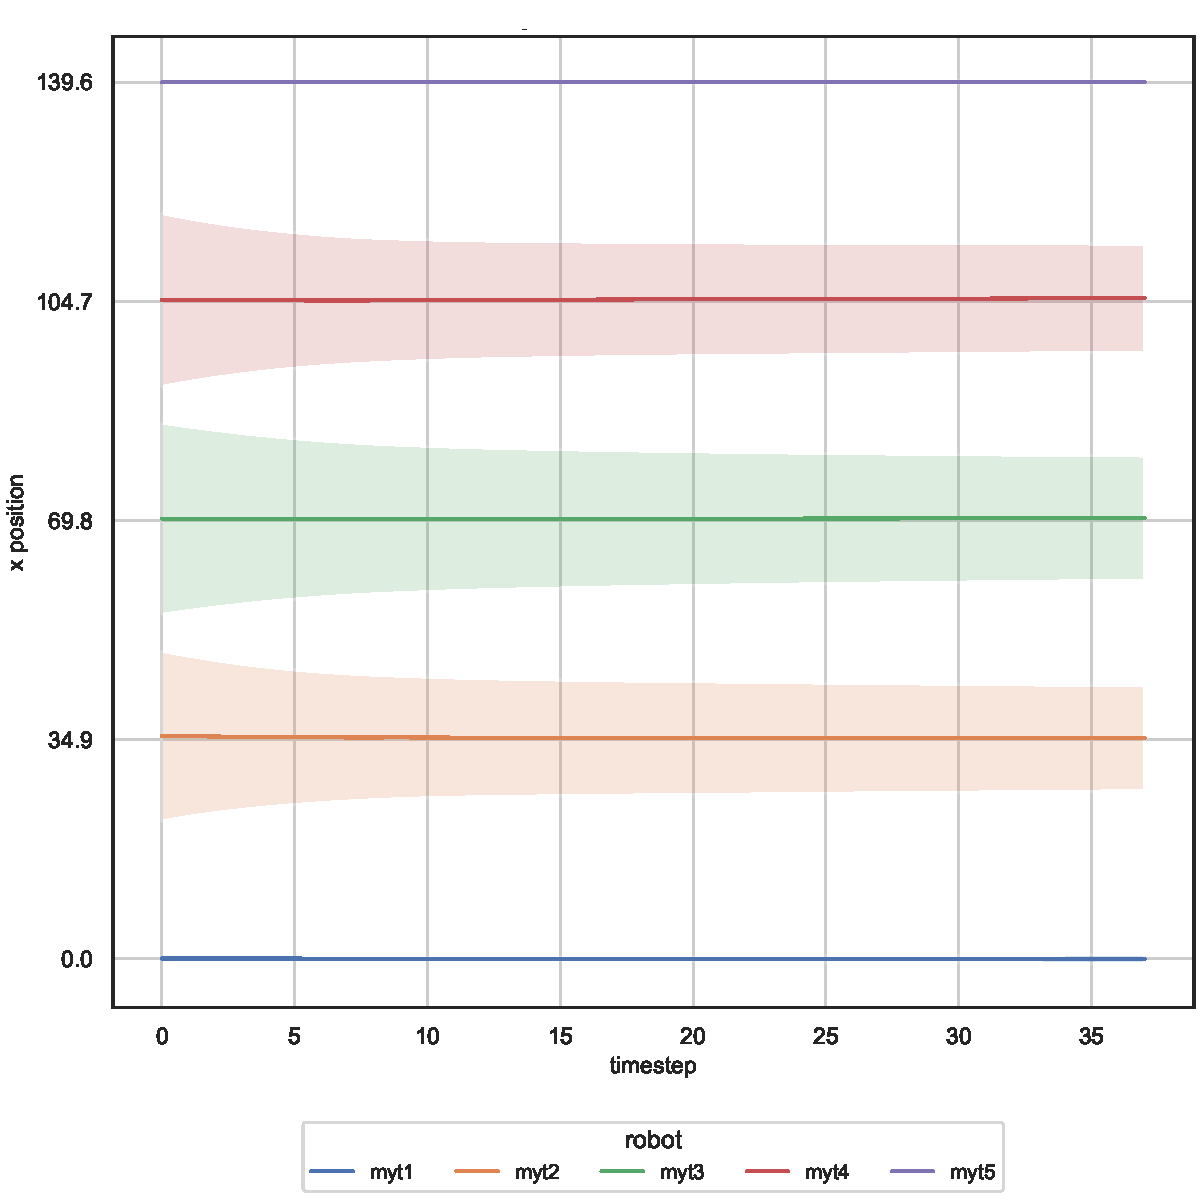
\includegraphics[width=.95\textwidth]{contents/images/net-d9/position-overtime-learned_distributed}
			\caption{Distributed controller trajectories.}
		\end{subfigure}
	\end{center}
	\caption[Evaluation of the trajectories learned by 
	\texttt{net-d9}.]{Comparison of trajectories generated using three controllers: 
	the expert, the manual and the one learned from \texttt{net-d9}.}
\end{figure}
\bigskip
\begin{figure}[!htb]\ContinuedFloat
	\centering
	\begin{subfigure}[h]{0.49\textwidth}
		\centering
		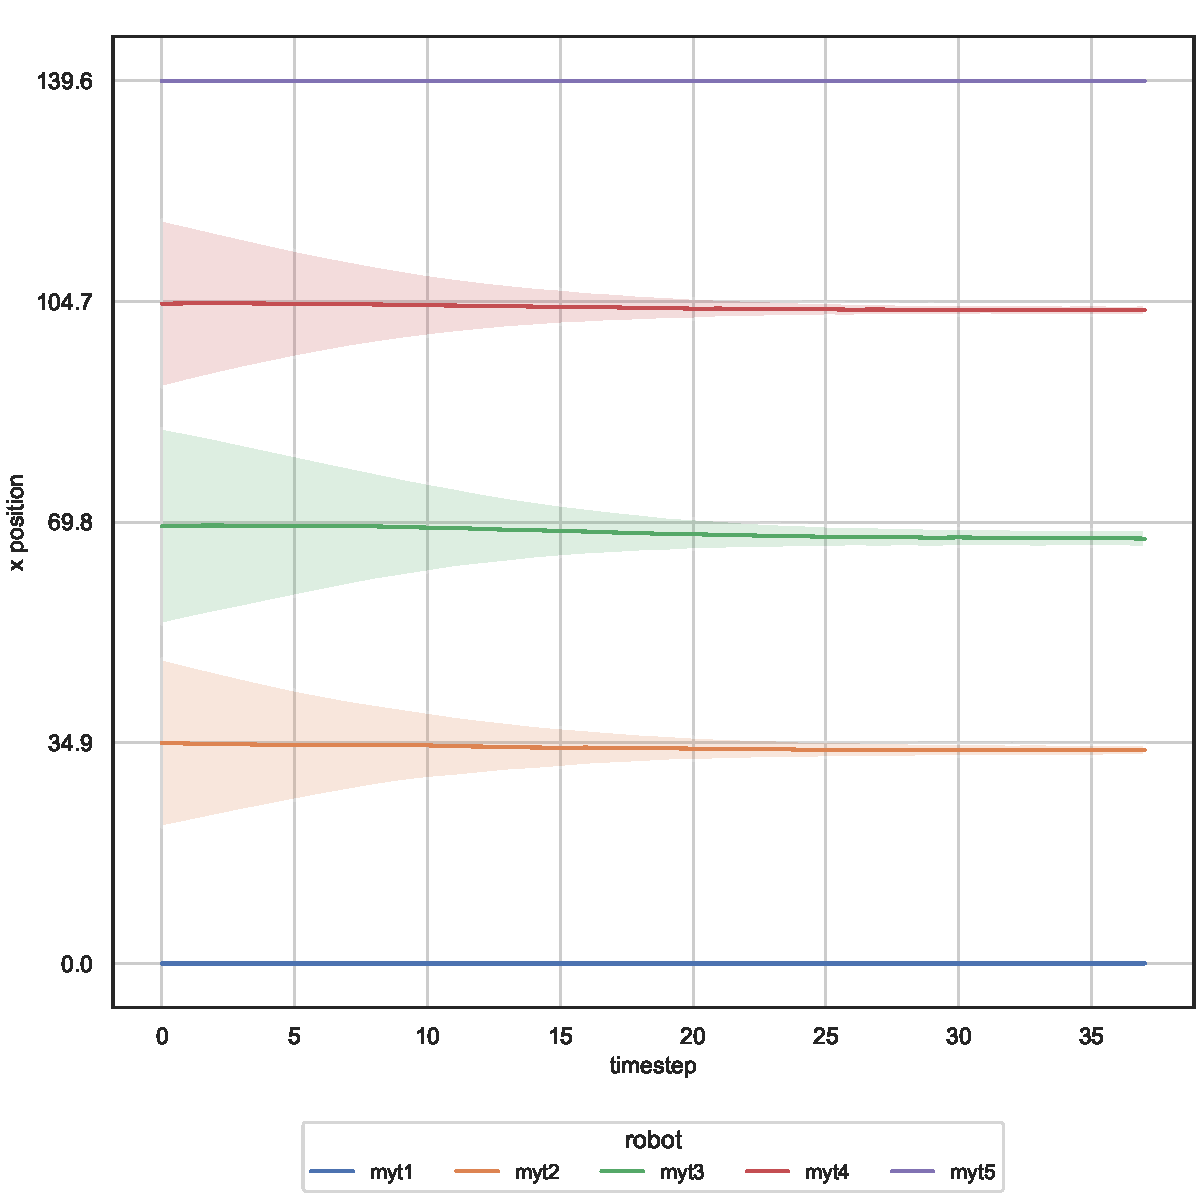
\includegraphics[width=.95\textwidth]{contents/images/net-d9/position-overtime-manual}%
		\caption{Manual controller trajectories.}
	\end{subfigure}
	\hfill
	\begin{subfigure}[h]{0.49\textwidth}
		\centering
		\includegraphics[width=.95\textwidth]{contents/images/net-d9/position-overtime-learned_distributed}
		\caption{Distributed controller trajectories.}
	\end{subfigure}
	\caption[]{Comparison of trajectories generated using three controllers: the 
	expert, the manual and the one learned from \texttt{net-d9} (cont.).}
	\label{fig:net-d9traj}
\end{figure}
\begin{figure}[!htb]
	\centering
	\begin{subfigure}[h]{0.3\textwidth}
		\centering
		\includegraphics[width=\textwidth]{contents/images/net-d9/control-overtime-omniscient}%
		\caption{Expert controller.}
	\end{subfigure}
	\hfill
	\begin{subfigure}[h]{0.3\textwidth}
		\centering
		\includegraphics[width=\textwidth]{contents/images/net-d9/control-overtime-manual}%
		\caption{Manual controller.}
	\end{subfigure}
	\hfill
	\begin{subfigure}[h]{0.3\textwidth}
		\centering
		\includegraphics[width=\textwidth]{contents/images/net-d9/control-overtime-learned_distributed}
		\caption{Distributed controller.}
	\end{subfigure}
	\caption[Evaluation of the control decided by \texttt{net-d9}.]{Comparison 
		of output control decided using three controllers: the expert, the manual 
		and the one learned from \texttt{net-d9}.}
	\label{fig:net-d9control}
\end{figure}


\begin{figure}[!htb]
	\centering
	\includegraphics[width=.45\textwidth]{contents/images/net-d9/response-varying_init_position-distributed}%
	\caption{Response of \texttt{net-d9} by varying the initial position.}
	\label{fig:net-d9responseposition}
\end{figure}


Finally, in Figure \ref{fig:net-d9distance} is presented the absolute distance of 
each robot from the target, averaged on all robots among all the simulation runs. 
The median value is shown as well as the interquartile and interdecile ranges.
\begin{figure}[!htb]
	\centering
	\includegraphics[width=.65\textwidth]{contents/images/net-d9/distances-from-goal-compressed-distributed}%
	\caption[Evaluation of \texttt{net-d9} distances from goal.]{Comparison of 
		performance in terms of distances from goal obtained using three 
		controllers: the expert, the manual and the one learned from \texttt{net-d9}.}
	\label{fig:net-d9distance}
\end{figure}
As anticipated by the trajectories in Figure \ref{fig:net-d9traj}, the controller 
learned from \texttt{net-d9} is slower to converge than the manual one. In fact, 
this plot confirms that the agents moved following a manual controller in the final 
configuration are closer to the target than those moved by the distributed 
controller, respectively, they are on average $2$ or $7$\gls{cm} away from the 
goal position.

\begin{figure}[!htb]
	\centering
	\begin{subfigure}[h]{0.3\textwidth}
		\centering
		\includegraphics[width=\textwidth]{contents/images/task1/loss-distributed-gap_8@copy}%
		\caption{\texttt{avg\_gap} of $8$\gls{cm}.}
	\end{subfigure}
	\hfill
	\begin{subfigure}[h]{0.3\textwidth}
		\centering
		\includegraphics[width=\textwidth]{contents/images/task1/loss-distributed-gap_13@copy}%
		\caption{\texttt{avg\_gap} of $13$\gls{cm}.}
	\end{subfigure}
	\hfill
	\begin{subfigure}[h]{0.3\textwidth}
		\centering
		\includegraphics[width=\textwidth]{contents/images/task1/loss-distributed-gap_24@copy}
		\caption{\texttt{avg\_gap} of $24$\gls{cm}.}
	\end{subfigure}
	\caption[Losses summary of the first set of experiments.]{Comparison 
	of the losses by varying the input of the networks for the three gaps.}
	\label{fig:distloss81324}
\end{figure}

\medskip
To summarise the performance, as the different inputs of the network vary, for 
each gap, we show once again in the figures below the losses of the trained 
models. In all the figures the blue line represents the loss using 
\texttt{prox\_values} as input, in orange \texttt{prox\_comm} and finally in green 
\texttt{all\_sensors}.
In case of an \texttt{avg\_gap} of $8$\gls{cm}, the model trained using 
\texttt{prox\_values} as input has a lower loss, following is the network that 
employ \texttt{all\_sensors}, with a very similar value, and at the end the model 
that works with \texttt{prox\_comm}.
It is quite obvious that the performance obtained using as inputs 
\texttt{prox\_values} and \texttt{all\_sensors} are the best, as well as the fact that 
\texttt{all\_sensors} cannot perform better than \texttt{prox\_values} with small 
gaps, since in this case the data coming from \texttt{prox\_comm} contains only 
zeros in the the second half of the array, making it unusable.
In a complementary way, by increasing the gap to $13$\gls{cm},  
\texttt{prox\_values} alone is not able to achieve satisfactory results, while used 
together with \texttt{prox\_comm}, \texttt{all\_sensors} reaches good 
performances that on the validation set are comparable to those obtained using 
\texttt{prox\_comm} alone.
Finally, by increasing the gap even more, up to $24$\gls{cm}, 
\texttt{prox\_values} becomes completely unusable, while \texttt{prox\_comm} 
and \texttt{all\_sensors} still have excellent performances similar to each other.

The last group of experiments we carried out using a distributed approach, 
examines the behaviour of the control learned using \texttt{all\_sensors} 
inputs. In this situation the simulation runs use a different number of robots $N$, 
that can be fixed at $5$ or $8$ for the entire simulation, or even vary in the range 
$[5, 10]$. The same reasoning is applied for the choice of the \texttt{avg\_gap}, 
that can be a fixed value in all the runs, chosen between $8$ or $20$, but also 
vary in the range $[5, 24]$. 
The objective of this set of experiments, summarised in Table \ref{tab:modeldist}, 
is to verify the robustness of the models, proving that it is possible to train 
networks that handle a variable number of agents. 
\begin{figure}[H]
	\centering
	\begin{tabular}{ccccc}
		\toprule
		\textbf{Model} \quad & \textbf{\texttt{network\_input}} & 
		\textbf{\texttt{input\_size}} & \textbf{\texttt{avg\_gap}} & \textbf{\texttt{N}}\\
		\midrule
		\texttt{net-d10} 	& \texttt{all\_sensors}		&  $14$  &  $8$		 	 &	$5$ \\
		\texttt{net-d11} 	& \texttt{all\_sensors}		&  $14$  &  $20$		&	$5$ \\
		\texttt{net-d12} 	& \texttt{all\_sensors}		&  $14$  &  variable   &	$5$ \\
		\texttt{net-d13} 	& \texttt{all\_sensors}	  	&  $14$  &  $8$			 &	  $8$ \\
		\texttt{net-d14} 	& \texttt{all\_sensors}	  	&  $14$  &  $20$   		&	 $8$ \\
		\texttt{net-d15} 	& \texttt{all\_sensors}	  	&  $14$  &  variable	&	 $8$ \\
		\texttt{net-d16} 	& \texttt{all\_sensors}	  	&  $14$  &  $ 8$		  &	 variable\\
		\texttt{net-d17} 	& \texttt{all\_sensors}	  	&  $14$  &  $20$		 &	variable\\
		\texttt{net-d18} 	& \texttt{all\_sensors}	  	&  $14$  &  variable	 &	
		variable\\
		\bottomrule
	\end{tabular}
	\captionof{table}[Experiments with variable agents and gaps (no 
	communication).]{List of the experiments carried out using a variable 
	number of agents and of gap.}
	\label{tab:modeldist}
\end{figure}

First of all we start by showing in Figure \ref{fig:distlossext} an overview of the 
models performance in terms of train and validation losses and in Figure 
\ref{fig:distlossn5} an analysis on the experiments performed using a fixed 
number of agents, the same used for the group of experiments presented above, 
i.e. $5$, in order to show the difference of performance using a gap that is first 
small, then large and finally variable.
\begin{figure}[!htb]
	\centering
	\includegraphics[width=.8\textwidth]{contents/images/task1-extension/loss-distributed-all@}%
	\caption[Comparison of losses of the second set of 
	experiments.]{Comparison of the losses of the models carried out using a 
	variable number of agents and of average gap.}
	\label{fig:distlossext}
\end{figure}
\begin{figure}[!htb]
	\centering
	\includegraphics[width=.8\textwidth]{contents/images/task1-extension/loss-distributed-N5@}%
	\caption{Comparison of the losses of the models that use $5$ agents as the gap 
	varies.}
	\label{fig:distlossn5}
\end{figure}

\begin{figure}[!htb]
	\centering
	\begin{subfigure}[h]{0.49\textwidth}
		\centering
		\includegraphics[width=\textwidth]{contents/images/net-d12/regression-manualvsomniscient}%
	\end{subfigure}
	\hfill
	\begin{subfigure}[h]{0.49\textwidth}
		\centering
		\includegraphics[width=\textwidth]{contents/images/net-d12/regression-net-d12-vs-omniscient}
	\end{subfigure}
	\caption[Evaluation of the \gls{r2} coefficients of \texttt{net-d12} 
	.]{Comparison 
		of the \gls{r2} coefficients of the manual and the controller learned from 
		\texttt{net-d12} with respect to the omniscient one.}
	\label{fig:net-d12r2}
\end{figure}

Examining more in detail the case in which the model is trained using a 
variable average gap, in Figure \ref{fig:net-d12r2} is visualised a comparison of 
the \gls{r2} of the manual and the learned controllers, on the validation set. 
The robots' behaviour using the learned instead of the manual controller is a 
bit better, even if far from the expert.

In Figure \ref{fig:net-d12traj} we show first a comparison of the expert and the 
learned trajectories, and then between the manual and the learned ones. 
In particular, on the y-axis is visualised the position of each agent over time, 
averaged over all the simulation runs, while on the x-axis the simulation 
time steps. 
\begin{figure}[!htb]
	\begin{center}
		\begin{subfigure}[h]{0.49\textwidth}
			\centering
			\includegraphics[width=.95\textwidth]{contents/images/net-d12/position-overtime-omniscient}%
			\caption{Expert controller trajectories.}
		\end{subfigure}
		\hfill
		\begin{subfigure}[h]{0.49\textwidth}
			\centering
			\includegraphics[width=.95\textwidth]{contents/images/net-d12/position-overtime-learned_distributed}
			\caption{Distributed controller trajectories.}
		\end{subfigure}
	\end{center}
	\begin{center}
		\begin{subfigure}[h]{0.49\textwidth}
			\centering			
			\includegraphics[width=.95\textwidth]{contents/images/net-d12/position-overtime-manual}%
			\caption{Manual controller trajectories.}
		\end{subfigure}
		\hfill
		\begin{subfigure}[h]{0.49\textwidth}
			\centering
			\includegraphics[width=.95\textwidth]{contents/images/net-d12/position-overtime-learned_distributed}
			\caption{Distributed controller trajectories.}
		\end{subfigure}
	\end{center}
	\vspace{-0.5cm}
	\caption[Evaluation of the trajectories learned by 
	\texttt{net-d12}.]{Comparison of trajectories generated using three controllers: 
		the expert, the manual and the one learned from \texttt{net-d12} (cont.).}
	\label{fig:net-d12traj}
\end{figure}
It is important to note that there is a difference in these graphs compared to 
those of the previous group of experiments. Observing the deviation of the 
position of the robots with respect to the average, the last agent of the row did 
not maintain the same initial and goal positions throughout the simulations since 
the average gap set is different for every run.
The convergence of the robots to the target is guaranteed in 20 time steps using 
the expert, while the manual and learned controller still manage to reach the 
correct configuration with more time.

Analysing the evolution of the control over time, in Figure 
\ref{fig:net-d12control}, we observe that the speeds set by the manual controller 
and the one learned from the network are significantly lower and therefore do 
not allow to reach the target in a satisfactory time.
\begin{figure}[!htb]
	\centering
	\begin{subfigure}[h]{0.3\textwidth}
		\centering
		\includegraphics[width=\textwidth]{contents/images/net-d12/control-overtime-omniscient}%
		\caption{Expert controller.}
	\end{subfigure}
	\hfill
	\begin{subfigure}[h]{0.3\textwidth}
		\centering
		\includegraphics[width=\textwidth]{contents/images/net-d12/control-overtime-manual}%
		\caption{Manual controller.}
	\end{subfigure}
	\hfill
	\begin{subfigure}[h]{0.3\textwidth}
		\centering
		\includegraphics[width=\textwidth]{contents/images/net-d12/control-overtime-learned_distributed}
		\caption{Distributed controller.}
	\end{subfigure}
	\caption[Evaluation of the control decided by \texttt{net-d12}.]{Comparison 
		of output control decided using three controllers: the expert, the 
		manual and the one learned from \texttt{net-d12}.}
	\label{fig:net-d12control}
\end{figure}

In Figure \ref{fig:net-d12responseposition} another informative plot displays 
the behaviour of a robot located between two that are already in their place.
As expected, the trend of the three curves shows how the behaviour of the 
model learned and of the manual controller are similar.
\begin{figure}[!htb]
	\centering
	\includegraphics[width=.45\textwidth]{contents/images/net-d12/response-varying_init_position-distributed}%
	\caption{Response of \texttt{net-d12} by varying the initial position.}
	\label{fig:net-d12responseposition}
\end{figure}


Finally, in Figure \ref{fig:net-d12distance} is shown the absolute distance of 
each robot from the target, averaged on all robots among all the simulation runs, 
over time. 
Despite we expected performances similar to those presented in the Figure 
\ref{fig:net-d9distance}, in this circumstance the agents moved following the 
distributed controller are closer to the target, in particular in the final 
configuration they are on average $2$\gls{cm} away from the goal position. 
Furthermore, it is shown that there are far fewer cases far from average 
behaviour.
\begin{figure}[!htb]
	\centering
	\includegraphics[width=.65\textwidth]{contents/images/net-d12/distances-from-goal-compressed-distributed}%
	\caption[Evaluation of \texttt{net-d1} distances from goal.]{Comparison of 
		performance in terms of distances from goal obtained using three 
		controllers: 
		the expert, the manual and the one learned from \texttt{net-d12}.}
	\label{fig:net-d12distance}
\end{figure}

Following are shown the losses of the models trained using an higher number of 
agents, i.e. 8, by varying the average gap.
In Figure \ref{fig:distlossprox_comm}, are analysed. From a first observation 
the network seems to be able to work with all the gaps.
\begin{figure}[!htb]
	\centering
	\includegraphics[width=.75\textwidth]{contents/images/task1-extension/loss-distributed-n8@}%
	\caption{Comparison of the losses of the models that use $8$ agents as 
	the gap 
	varies.}
	\label{fig:distlossn8}
\end{figure}
As before, for the network it is easier to perform a task using a smaller gap.
For this reason, it is more interesting to analyse the case in which the model 
is trained using a variable gap.

In Figure \ref{fig:net-d15r2} is visualised a comparison of the \gls{r2} 
coefficients of the manual and the learned controller. In both cases, the 
coefficients are very low, since in most of the cases in which the controllers have 
to decide a zero or maximum speed a wrong value is predicted, however, the 
coefficient obtained from the network is slightly better.
\begin{figure}[!htb]
	\centering
	\begin{subfigure}[h]{0.49\textwidth}
		\centering
		\includegraphics[width=\textwidth]{contents/images/net-d15/regression-manualvsomniscient}%
	\end{subfigure}
	\hfill
	\begin{subfigure}[h]{0.49\textwidth}
		\centering
		\includegraphics[width=\textwidth]{contents/images/net-d15/regression-net-d15-vs-omniscient}
	\end{subfigure}
	\caption[Evaluation of the \gls{r2} coefficients of \texttt{net-d15} 
	.]{Comparison of the \gls{r2} coefficients of the manual and the controller 
		learned from \texttt{net-d15} with respect to the omniscient one.}
	\label{fig:net-d15r2}
\end{figure}

In Figure \ref{fig:net-d15traj} are shown the trajectories obtained employing 
the three controllers. 
Compared to the previous case, a greater number of robots implies a 
slowdown in reaching the correct position, even when using an expert 
controller.
As before, the convergence of the robots using the manual and learned 
controllers needs more time.

Examining in Figure \ref{fig:net-d15control} the evolution of the control over 
time, the graph of the distributed controller highlights how the speed decided by 
the model has further decreased due to the increase in the amount of agents in 
the simulation.

\begin{figure}[!htb]
	\begin{center}
		\begin{subfigure}[h]{0.49\textwidth}
			\centering
			\includegraphics[width=.9\textwidth]{contents/images/net-d15/position-overtime-omniscient}%
			\caption{Expert controller trajectories.}
		\end{subfigure}
		\hfill
		\begin{subfigure}[h]{0.49\textwidth}
			\centering
			\includegraphics[width=.9\textwidth]{contents/images/net-d15/position-overtime-learned_distributed}
			\caption{Distributed controller trajectories.}
		\end{subfigure}
	\end{center}
	\caption[Evaluation of the trajectories learned by 
	\texttt{net-d15}.]{Comparison of trajectories generated using three controllers: 
		the expert, the manual and the one learned from \texttt{net-d15}.}
\end{figure}
\begin{figure}[!htb]\ContinuedFloat
	\begin{center}
		\begin{subfigure}[h]{0.49\textwidth}
			\centering			
			\includegraphics[width=.9\textwidth]{contents/images/net-d15/position-overtime-manual}%
			\caption{Manual controller trajectories.}
		\end{subfigure}
		\hfill
		\begin{subfigure}[h]{0.49\textwidth}
			\centering
			\includegraphics[width=.9\textwidth]{contents/images/net-d15/position-overtime-learned_distributed}
			\caption{Distributed controller trajectories.}
		\end{subfigure}
	\end{center}
	\caption[]{Comparison 
		of trajectories generated using three controllers: the expert, the manual 
		and the one learned from \texttt{net-d15}.}
	\label{fig:net-d15traj}
\end{figure}


\begin{figure}[!htb]
	\centering
	\begin{subfigure}[h]{0.3\textwidth}
		\centering
		\includegraphics[width=\textwidth]{contents/images/net-d15/control-overtime-omniscient}%
		\caption{Expert controller.}
	\end{subfigure}
	\hfill
	\begin{subfigure}[h]{0.3\textwidth}
		\centering
		\includegraphics[width=\textwidth]{contents/images/net-d15/control-overtime-manual}%
		\caption{Manual controller.}
	\end{subfigure}
	\hfill
	\begin{subfigure}[h]{0.3\textwidth}
		\centering
		\includegraphics[width=\textwidth]{contents/images/net-d15/control-overtime-learned_distributed}
		\caption{Distributed controller.}
	\end{subfigure}
	\caption[Evaluation of the control decided by \texttt{net-d15}.]{Comparison 
		of output control decided using three controllers: the expert, the manual 
		and the one learned from \texttt{net-d15}.}
	\label{fig:net-d15control}
\end{figure}

Figure \ref{fig:net-d15responseposition} displays the behaviour of a robot 
located between two that are already in their place.

\begin{figure}[!htb]
	\centering
	\includegraphics[width=.45\textwidth]{contents/images/net-d15/response-varying_init_position-distributed}%
	\caption{Response of \texttt{net-d15} by varying the initial position.}
	\label{fig:net-d15responseposition}
\end{figure}

Analysing the way of acting of the three controllers for this experiment, from 
the plot arises an important difference in the decisions taken by the distributed 
and the manual controllers.
The learned controller, whether a robot is closer to the one that precedes it 
or to the one following it, sets a proportional speed, lower than the optimal one, 
that leads it to move respectively back and forth to reach the desired position.
Instead, the manual controller when an agent is closer to the one in front 
sets a very high speed to move quickly to the desired position, just like the expert 
does, unlike when the robot is closer to the one following it, where it sets a 
negative speed but not high enough, a bit like the distributed controller does.

Finally, in Figure \ref{fig:net-d15distance} is presented the average distance of 
the robots from the target among all the simulations. The performance of the 
learned and the manual controllers 
\begin{figure}[!htb]
	\centering
	\includegraphics[width=.65\textwidth]{contents/images/net-d15/distances-from-goal-compressed-distributed}%
	\caption[Evaluation of \texttt{net-d15} distances from goal.]{Comparison 
	of performance in terms of distances from goal obtained using three 
	controllers: the expert, the manual and the one learned from \texttt{net-d15}.}
	\label{fig:net-d15distance}
\end{figure}

\noindent
are different from before: \texttt{net-d15} is slower to converge. In fact, this plot 
confirms that the agents moved following a manual controller in the final 
configuration are closer to the target than those moved by the distributed 
controller, respectively, they are on average $2$ or $3.5$\gls{cm} away from the 
goal position. Moreover, observing the coloured bands we see that there is a lot of 
variance in the distributed controller final positions, in fact there are runs in which 
some agents can be even $10$\gls{cm} far from the target.

\bigskip
We conclude the experiments performed using a distributed approach by 
presenting the results obtained with a number of agents variable. 
In Figure \ref{fig:distlossnvar}, are analysed the losses by varying the average 
gap. As before, for the network it is easier to perform a task using a smaller gap 
and in general training the model on a variable gap performs better than on a 
fixed but big gap.
\begin{figure}[!htb]
	\centering
	\includegraphics[width=.9\textwidth]{contents/images/task1-extension/loss-distributed-Nvar@}%
	\caption{Comparison of the losses of the models that use variable agents and 	
	gaps.}
	\label{fig:distlossnvar}
\end{figure}

Dwelling on the most interesting case, the one in with both average gap and 
number of agents variable, the \gls{r2} coefficients shown in Figure 
\ref{fig:net-d18r2} are still very low.
\begin{figure}[!htb]
	\centering
	\begin{subfigure}[h]{0.49\textwidth}
		\centering
		\includegraphics[width=\textwidth]{contents/images/net-d18/regression-manualvsomniscient}%
	\end{subfigure}
	\hfill
	\begin{subfigure}[h]{0.49\textwidth}
		\centering
		\includegraphics[width=\textwidth]{contents/images/net-d18/regression-net-d18-vs-omniscient}
	\end{subfigure}
	\caption[Evaluation of the \gls{r2} coefficients of \texttt{net-d18} 
	.]{Comparison of the \gls{r2} coefficient of the manual and the controller 
	learned from \texttt{net-d18} with respect to the omniscient one.}
	\label{fig:net-d18r2}
\end{figure}

Since the number of agents is variable, we show different plots, depending on this 
quantity, for the trajectories obtained employing the three controllers: we analyse 
the cases with 5, 8 and 10 agents respectively in Figures \ref{fig:net-d18traj5}, 
\ref{fig:net-d18traj8} and \ref{fig:net-d18traj10}. 
\begin{figure}[!htb]
	\begin{center}
		\begin{subfigure}[h]{0.325\textwidth}
			\centering
			\includegraphics[width=\textwidth]{contents/images/net-d18/N5/position-overtime-omniscient}%
			\caption{Expert controller.}
		\end{subfigure}
		\hfill
		\begin{subfigure}[h]{0.325\textwidth}
			\centering
			\includegraphics[width=\textwidth]{contents/images/net-d18/N5/position-overtime-manual}%
			\caption{Manual controller.}
		\end{subfigure}
		\hfill
		\begin{subfigure}[h]{0.325\textwidth}
			\centering
			\includegraphics[width=\textwidth]{contents/images/net-d18/N5/position-overtime-distributed}
			\caption{Distributed controller.}
		\end{subfigure}
	\end{center}
	\caption[Evaluation of the trajectories learned by \texttt{net-d18} using 5 
	agents.]{Comparison of trajectories of 5 agents generated using three 
		controllers.}
	\label{fig:net-d18traj5}
\end{figure}
\begin{figure}[!htb]
	\begin{center}
		\begin{subfigure}[h]{0.325\textwidth}
			\centering
			\includegraphics[width=\textwidth]{contents/images/net-d18/N8/position-overtime-omniscient}%
			\caption{Expert controller.}
		\end{subfigure}
		\hfill
		\begin{subfigure}[h]{0.325\textwidth}
			\centering
			\includegraphics[width=\textwidth]{contents/images/net-d18/N8/position-overtime-manual}%
			\caption{Manual controller.}
		\end{subfigure}
		\hfill
		\begin{subfigure}[h]{0.325\textwidth}
			\centering
			\includegraphics[width=\textwidth]{contents/images/net-d18/N8/position-overtime-distributed}
			\caption{Distributed controller.}
		\end{subfigure}
	\end{center}
	\caption[Evaluation of the trajectories learned by \texttt{net-d18} using 8 
	agents.]{Comparison of trajectories of 8 agents generated using three 
		controllers.}
	\label{fig:net-d18traj8}
\end{figure}
\begin{figure}[!htb]
	\begin{center}
		\begin{subfigure}[h]{0.325\textwidth}
			\centering
			\includegraphics[width=\textwidth]{contents/images/net-d18/N10/position-overtime-omniscient}%
			\caption{Expert controller.}
		\end{subfigure}
		\hfill
	\begin{subfigure}[h]{0.325\textwidth}
		\centering
		\includegraphics[width=\textwidth]{contents/images/net-d18/N10/position-overtime-manual}%
		\caption{Manual controller.}
	\end{subfigure}
	\hfill
	\begin{subfigure}[h]{0.325\textwidth}
		\centering
		\includegraphics[width=\textwidth]{contents/images/net-d18/N10/position-overtime-distributed}
		\caption{Distributed controller.}
	\end{subfigure}
\end{center}
	\caption[Evaluation of the trajectories learned by \texttt{net-d18} using 10 
	agents.]{Comparison of trajectories of 10 agents generated using three 
	controllers.}
	\label{fig:net-d18traj10}
\end{figure}

\noindent
From a first observation it is confirmed that increasing the number of robots in 
the simulation implies a greater number of time steps to reach the final 
configuration.
Furthermore, with a large number of agents it is common for biases to add up 
and for the error to become more significant, in particular the one of the central 
robot of the group.
The convergence is still slow, even if this time the expert need less time steps than 
before. The learned controller is still the slowest to end up in the correct 
configuration.

Examining the evolution of the output control, in Figure \ref{fig:net-d18control}, 
the graph of the distributed controller highlights how the speed decided by the 
model has decreased due to the increase in the amount of agents in the 
simulation.
\begin{figure}[!htb]
	\centering
	\begin{subfigure}[h]{0.3\textwidth}
		\centering
		\includegraphics[width=\textwidth]{contents/images/net-d18/control-overtime-omniscient}%
		\caption{Expert controller.}
	\end{subfigure}
	\hfill
	\begin{subfigure}[h]{0.3\textwidth}
		\centering
		\includegraphics[width=\textwidth]{contents/images/net-d18/control-overtime-manual}%
		\caption{Manual controller.}
	\end{subfigure}
	\hfill
	\begin{subfigure}[h]{0.3\textwidth}
		\centering
		\includegraphics[width=\textwidth]{contents/images/net-d18/control-overtime-learned_distributed}
		\caption{Distributed controller.}
	\end{subfigure}
	\caption[Evaluation of the control decided by \texttt{net-d18}.]{Comparison 
		of output control decided using three controllers: the expert, the manual and 
		the one learned from \texttt{net-d18}.}
	\label{fig:net-d18control}
\end{figure}

In Figure \ref{fig:net-d18responseposition} is displayed the behaviour of a robot 
located between two that are already in their place.
\begin{figure}[!htb]
	\centering
	\includegraphics[width=.45\textwidth]{contents/images/net-d18/response-varying_init_position-distributed}%
	\caption{Response of \texttt{net-d18} by varying the initial position.}
	\label{fig:net-d18responseposition}
\end{figure}
In this case the same reasoning made for Figure 
\ref{fig:net-d15responseposition} apply.

Focusing on the absolute distance of each robot from the target, presented in 
Figure \ref{fig:net-d18distance}, we observe once again that the agents moved 
following a manual controller in the final configuration are closer to the target 
than those moved with the learned one.
\begin{figure}[!htb]
	\centering
	\includegraphics[width=.65\textwidth]{contents/images/net-d18/distances-from-goal-compressed-distributed}%
	\caption[Evaluation of \texttt{net-d18} distances from goal.]{Comparison of 
		performance in terms of distances from goal obtained using three 
		controllers: the expert, the manual and the one learned from 
		\texttt{net-d18}.}
	\label{fig:net-d18distance}
\end{figure}

\bigskip
To summarise the performance, as the number of agents vary for each gap, we 
show once again in the figures below the losses of the trained models.
In case of an \texttt{avg\_gap} of $8$\gls{cm}, the model trained using 
a minor number of agents, as expected has a lower loss, following, with very 
similar values the model that employ 8 robots and that with a variable number of 
agents.
Finally, by choosing a variable gap and number of agents the performance are 
better than those generated with fixed but high number of robots. While again, 
the results obtained using fewer agents are the best.
\begin{figure}[!htb]
	\centering
	\begin{subfigure}[h]{0.3\textwidth}
		\centering
		\includegraphics[width=\textwidth]{contents/images/task1-extension/loss-distributed-gap_8@copy}%
		\caption{\texttt{avg\_gap} of $8$\gls{cm}.}
	\end{subfigure}
	\hfill
	\begin{subfigure}[h]{0.3\textwidth}
		\centering
		\includegraphics[width=\textwidth]{contents/images/task1-extension/loss-distributed-gap_20@copy}%
		\caption{\texttt{avg\_gap} of $20$\gls{cm}.}
	\end{subfigure}
	\hfill
	\begin{subfigure}[h]{0.3\textwidth}
		\centering
		\includegraphics[width=\textwidth]{contents/images/task1-extension/loss-distributed-gap_var@copy}
		\caption{\texttt{avg\_gap} variable.}
	\end{subfigure}
		\caption[Losses summary of the second set of 
		experiments.]{Comparison of the losses by varying the input of the networks 
		for different gaps.}
	\label{fig:distloss820var}
\end{figure}
\vspace{-0.5cm}
\subsubsection{Summary}
\label{subsubsec:summary}
In this section we have shown that using a distributed controller learned by 
imitating an expert it is possible to obtain results more or less comparable to 
those reached employing a manual controller.
However, this approach is not enough to achieve satisfactory performance. In the 
following section we are going to describe a second approach that solve the 
problem by exploiting a communication protocol between agents.
\subsection{Distributed approach with communication}
\label{subsec:ex1comm}

\subsubsection{Model training}
\label{subsubsec:learnedcomm}
An alternative to the previous approach involves the possibility of training a 
new distributed network that exploit a communication protocol between 
agents to decide more reliably the output control.

Using the same data collected in the previous approach we build a model that 
at each timestep takes as input for each robot an array containing the 
response values of the sensors – which can be either \texttt{prox\_values}, 
\texttt{prox\_comm} or \texttt{all\_sensors} – and the message received in 
the previous timestep, communicated by the nearest agents (one on the left 
and one on the right), and produces as output an array of 2 floats, 
corresponding the first one to the control, which, as before, is the speed of 
the wheels, and the second one to the communication, i.e. the message 
transmitted by the robot to the nearest agents.

Also for this purpose, the model is independent of the number of agents in 
the simulations. Instead, in this approach is important to keep track of the 
timesteps order since the input of the network requires the communication 
received in the actual timestep which corresponds to a message transmitted 
in the previous one. 
To do so, a preprocessing is applied to the dataset in order to combine 
consecutive timesteps into a set of sequences. Therefore, we divide each 
simulation in sequences of length $2$, or composed by two consecutive 
timesteps, using a stride of $1$ among them, which contains an ordered 
series of two states for each robot.   

For this model the shape of the input has been transformed from $1 \times 
\mathtt{input\_size}$ to $\mathtt{seq\_length} \times \mathtt{N} \times 
\mathtt{input\_size}$, where \texttt{seq\_length} is fixed at $2$, $N$ is variable 
and \texttt{input\_size} can be $7$ or $14$.

It is important to notice that the communication is not yet in the input since 
it is not contained in the original dataset, instead is treated as a hidden 
variable to be inferred. 
At the beginning of each sequence there are no previous timesteps to 
consider since no messages have been received yet. Therefore, a placeholder 
is randomly initialised, filled with float values in the range $[0, 1]$. 
The size of this array corresponds to the number of agents plus two 
elements, one at the beginning and one at the end of the vector, always set 
to $0$, since they are used to store the fact that the two extreme robots 
never receive messages respectively from the left or from the right. 
The random initialisation of this vector is essential to increase the 
generalization capabilities of the network during its training, showing it 
different starting situations.

Another crucial aspect to consider when using communication is the type of   
updated protocol to choose. As we have already said in section 
\ref{subsec:thymiocomm}, each robot transmits a message every 0.1\gls{s} 
and likewise receives one for each of the sensors. In our case, we expect 
each agent to receive two communications, one for each of its respective 
neighbours. 
With real robots, but also in simulation, what we want to attain is a 
synchronous communication update protocol. Formally, each robot $n$, 
given the observations at time $t$, that correspond to the sensor readings 
$S_n(t)$, and the communications at time $t-1$, in particular $C_{n-1}(t-1)$ 
and $C_{n+1}(t-1)$, calculates the control $V_n(t)$ and the message to 
transmit $C_n(t)$. 
Adopting this policy it is not important to keep track of the order of the 
robots and it is as if the agents operate simultaneously. 
Ideally, the frequency of updates must be lower than that with which the 
robots exchange messages, however it can happen that due to delays or 
noise in the sensor readings the communication of some robots is not 
received or transmitted. In this case, the array is not updated and the last 
message received is keep instead. 

As a consequence, we define a recurrent structure of the communication 
network, shown in Figure \ref{fig:commnet1}. It is composed by two nested 
modules: in the high-level operates the \texttt{CommNet} that handle the 
sensing of all the agents, while in the low-level the \texttt{SingleNet} that 
works on the sensing and the communication received by a single agent in a 
certain timestep, producing as output the control and the communication to 
transmit. 
\begin{figure}[!htb]
	\centering
	\includegraphics[width=\textwidth]{contents/images/commnet2}
	\caption[Communication network.]{Visualisation of the forward pass of the 
		communication network with three agents and a sequence composed by two 
		timesteps.}
	\label{fig:commnet1}
\end{figure}

The architecture of the \texttt{SingleNet}, displayed in Figure 
\ref{fig:singlenetcomm1}, is almost the same as the one of the distributed 
model without communication: there are three linear layers each of size 
$\langle\mathtt{input\_size} + 2, 10\rangle$,  $\langle 10, 
10\rangle$ and $\langle 10, 2\rangle$, where \texttt{input\_size} is the sum 
of the shape of the sensing and the two communication values received, one 
from the left and one from the right.

\begin{figure}[!htb]
	\centering
	\begin{subfigure}[h]{0.495\textwidth}
		\centering
		\includegraphics[width=.8\textwidth]{contents/images/task1distributedcomm@4x}%
		\caption{\texttt{SingleNet} with $7$ input sensing.}
	\end{subfigure}
	\hfill
	\begin{subfigure}[h]{0.495\textwidth}
		\centering
		\includegraphics[width=.8\textwidth]{contents/images/task1distributed_allcomm@4x}
		\caption{\texttt{SingleNet} with $14$ input sensing.}
	\end{subfigure}
	\caption[Network architectures for the distributed approach with 
	communication.]{Visualisation of the network architecture chosen for the 
	distributed approach with communication in case of 7 or 14 inputs.}
	\label{fig:singlenetcomm1}
\end{figure}

As before, to the first and second layer is applied a Tanh non-linear 
activation function, while a sigmoid \cite[see][]{han1995influence}, shown in 
Figure \ref{fig:sigmoid}, is applied to the second dimension of the output, 
that is the value of the communication to transmit, in order to normalise it in 
the range $[0, 1]$ and its output is given by
\begin{Equation}[H]
	\centering
	\begin{equation}
	\sigma(x)= \frac{1}{1 + e - x}
	\end{equation}
	\caption{Sigmoid Function.}
	\label{eq:sigmoid}
\end{Equation}

\begin{figure}[!htb]
	\centering
	\includegraphics[width=.5\textwidth]{contents/images/sigmoid2}%
	\caption[Trend of the Sigmoid activation function.]{Trend of the Sigmoid 
	Function applied as a non-linear activation to the second output of the 
	network.}
	\label{fig:sigmoid}
\end{figure}

As before, we use Adam optimiser but with a smaller learning rate, $0.001$. 
We split the dataset in mini-batches, this time of size $10$ and then train 
the models for $500$ epochs. 

Finally we evaluate the goodness of the predicted control using the \gls{mse} 
loss function, while the communication is learned in an unsupervised way.
Since the network is fully connected, the communication affects directly the 
output, and consequently, the error minimised, even if it is computed using 
only the control. Improving the loss has an impact also on the 
communication latent variable: since the error is propagated through the 
internal network, in order to update the weight during the back-propagation 
step, that influences the 
communication.

\subsubsection{Experiments}
\label{subsubsec:expcomm}

In this section we explore the same experiments carried out for the distributed 
approach without communication, paying more attention to the cases with 
variable gaps and robots. 
The first analysis, summarised in Table \ref{tab:modeln5comm}, also in this case  
concerns the behaviour of the learned controllers in case of the three different 
inputs, \texttt{prox\_values}, \texttt{prox\_comm} or 
\texttt{all\_sensors}, for a number of robots $N$ and an \texttt{avg\_gap} both 
fixed respectively at $5$ and the second chosen between $8$, $13$ and $24$.
\begin{figure}[!htb]
	\centering
	\begin{tabular}{cccc}
		\toprule
		\textbf{Model} \quad & \textbf{\texttt{network\_input}} & 
		\textbf{\texttt{input\_size}} &
		\textbf{\texttt{avg\_gap}} \\
		\midrule
		\texttt{net-c1} 				 & \texttt{prox\_values}	&  $  7$  &  $  8$  \\
		\texttt{net-c2} 			 	 & \texttt{prox\_values}	&  $  7$  &  $13$ \\
		\texttt{net-c3} 				 & \texttt{prox\_values}	&  $  7$  &  $24$  \\
		\texttt{net-c4} 				 & \texttt{prox\_comm}	  &  $  7$  &  $  8$  \\
		\texttt{net-c5} 				 & \texttt{prox\_comm}	  &  $  7$  &  $13$  \\
		\texttt{net-c6} 				 & \texttt{prox\_comm}	  &  $  7$  &  $24$  \\
		\texttt{net-c7} 				 & \texttt{all\_sensors}	  &  $14$  &  $  8$  \\
		\texttt{net-c8} 				 & \texttt{all\_sensors}	  &  $14$  &  $13$ 	\\
		\texttt{net-c9} 				 & \texttt{all\_sensors}	  &  $14$  &  $24$ 	\\
		\bottomrule
	\end{tabular}
	\captionof{table}[Experiments with $5$ agents (communication).]{List of the 
	experiments carried out with $5$ agents using communication.}
	\label{tab:modeln5comm}
\end{figure}





\section{Task 2: Colouring the robots in space}
\label{sec:task2}

The second scenario tackles another multi-agent coordination task, assuming that 
the agents are divided into groups, their purpose is to colour themselves, by 
turning on their top \gls{rgb} \gls{led}, depending on their group membership. 
As for the previous task, the problem can be solved performing imitation 
learning, but the role of communication is fundamental. In fact, what makes the 
difference are not the distances perceived by the robot sensors but the messages 
exchanged between the agents, which are they only mean to determine their 
order. 
In this scenario, the two ``dead'' robots play an important role: they always 
communicate a message that indicates that they are the only two agents that 
receive communication just from one side.

\subsection{Distributed approach with communication}
\label{subsec:task2-exp-comm}

\subsubsection{Experiment 1: variable number of agents}
\label{subsubsec:task2-exp-comm-1}
In this section we explore the experiments carried out using the communication 
approach, in particular, examining the behaviour of the control learned from 9 
networks 
\begin{figure}[!htb]
	\centering
	\begin{tabular}{ccc}
		\toprule
		\textbf{Model} \quad & \textbf{\texttt{avg\_gap}} & \textbf{\texttt{N}}\\
		\midrule
		\texttt{net-v1}   &  $8$		 &	 $5$ \\
		\texttt{net-v2}   &  $20$		&	$5$ \\
		\texttt{net-v3}   &  variable   &    $5$\\
		\texttt{net-v4}   &  $8$		 &	  $8$ \\
		\texttt{net-v5}   & $20$   		&	 $8$ \\
		\texttt{net-v6}   &  variable	&	 $8$ \\
		\texttt{net-v7}   &  $ 8$		  &	 variable\\
		\texttt{net-v8}   &  $20$		 &	variable\\
		\texttt{net-v9}   &  variable	 &	variable\\
		\bottomrule
	\end{tabular}
	\captionof{table}[Experiments with variable agents and gaps 
	(communication).]{List of the experiments carried out using a variable number 
		of agents and of gap.}
	\label{tab:modelcommt2}
\end{figure}

\noindent
based on different simulation runs that use a number of robots $N$ that 
can be fixed at $5$ or $8$ for the entire simulation, or even vary in the range $[5, 
10]$, and an \texttt{avg\_gap} that can be a fixed value in all the runs, chosen 
between $8$ or $20$, but also vary in the range $[5, 24]$. 
The objective of this set of experiments, summarised in Table 
\ref{tab:modelcommt2}, is to verify the robustness of the communication 
protocol and prove also the scalability of the network on the number of agents.

First of all we start by showing in Figure \ref{fig:t2lossallt} an overview of the train 
and validation losses obtained for these models.
\begin{figure}[!htb]
	\centering
	\includegraphics[width=.8\textwidth]{contents/images/task2/loss-communication-all@}%
	\caption[Comparison of losses of the second set of experiments.]{Comparison 
		of the losses of the models carried out using a variable number of agents and 
		of average gap.}
	\label{fig:t2lossallt}
\end{figure}

\paragraph*{Results using 5 agents}

We start our examination by inspecting the behaviour of the network trained on 
simulations with variable average gap, i.e \texttt{net-v3}, \texttt{net-v6} and 
\begin{figure}[!htb]
	\centering
	\includegraphics[width=.45\textwidth]{contents/images/task2/loss-communication-N5}
	\caption[Comparison of the losses of the models that use $5$ 
	agents.]{Comparison of the losses of the models that use $5$ agents as 
		the gap varies.}
	\label{fig:commlossn5t2}
\end{figure}

\noindent
\texttt{net-v9} and we summarise in Figure \ref{fig:commlossn5t2} the losses of 
these experiments in order to highlight the difference of performance using a gap 
that is first small, then large and finally variable, respectively represented by the 
blue, the orange and the green lines.
Clearly, in case of small gaps the network performs better, albeit slightly, as the 
agents are already close to the target.

Then, we move to explore the results of the experiments by showing in Figure 
\ref{fig:net-v3auc} the \gls{roc} curve of the model 
\cite[][]{fawcett2006introduction}, a visualisation of the performance of our 
classification model, in terms of \gls{tpr} versus \gls{fpr}, at all classification 
thresholds.
In particular we use the \gls{auc} to evaluate the classifier: by measuring the 
\gls{2d} area under the ROC curve, from $[0, 0]$ to $[1, 1]$, the \gls{auc} is able 
to provide an aggregate measure of performance as the discrimination threshold 
varies.
We assume that a model whose predictions are 100\% correct has an \gls{auc} of 
1, as in this case.
\begin{figure}[!htb]
	\centering
	\includegraphics[width=.5\textwidth]{contents/images/net-v3/roc-net-v3(a)}%
	\caption[Evaluation of the ROC of \texttt{net-v3}.]{Visualisation of the 
		\gls{roc} curve of \texttt{net-v3}.}
	\label{fig:net-v3auc}
\end{figure}x

Also for this task it is interesting to analyse the type of communication protocol 
inferred by the network, also comparing it with the one implemented by the 
manual controller. 
In Figure \ref{fig:net-v3commcolour} are shown, for a simulation run, first the 
messages transmitted by the agents over time, through a colour bar whose 
spectrum is included in the range [0, 1], i.e. the maximum and minimum value of 
communication transmitted, and then the colour assumed by the robot in a 
certain time step, for both the manual and the learned controllers.
The extreme robots always transmit the same message using both controllers, 
while using the learned one, the central robots seems to transmit the same value, 
i.e. 1, but despite this they are able to achieve their goal in only two time steps, 
one less than with the manual. This behaviour cannot scale to a number of robot 
higher then $5$. For instance, in case of $5$ agents, in the first time step, 
\texttt{myt2} and \texttt{myt4} receive respectively the messages $(0, 1)$ and $(1, 
0)$, so they immediately know their position with respect to the central robot, 
which in turn knows its position since it receives $(1, 1)$. Then they communicate 
their message and in the following time step all the agents have coloured 
themselves in the right way, achieving the goal.
Consequently if the number of robots is greater, the central robots are not able to 
localise themselves. 
\begin{figure}[!htb]
	\begin{subfigure}[h]{\textwidth}
		\centering
		\includegraphics[width=.6\textwidth]{contents/images/net-v3/net-v3-manual-0(1)}
		\caption{Communication and colour decided using the manual controller.}
	\end{subfigure}
	\hspace*{\fill}%          % empty line absolutely necessary!
	\vspace*{8pt}%  
	\hspace*{\fill}%  
	\begin{subfigure}[h]{\textwidth}
		\centering			
		\includegraphics[width=.6\textwidth]{contents/images/net-v3/net-v3-learned-0(1)}
		\caption{Communication and colour decided using the learned controller.}
	\end{subfigure}
	\caption[Evaluation of the communication learned by 
	\texttt{net-v3}.]{Visualisation of the communication transmitted by each 
		robot over time and the colour decided by the controller learned from 
		\texttt{net-v3}.}	
	\label{fig:net-v3commcolour}
\end{figure}
\vspace{0.5cm}

In Figure \ref{fig:net-v3error} is presented a useful metric that measures the 
amount of wrong expected colours, on the y-axis, over time, averaged for all the 
robots among the simulation runs. In particular, at each time step we count the 
number of agents that have the wrong colour and divide it by the number of 
simulations.
The mean value is shown as well as the bands representing minus and plus the 
standard deviation.
On average, the amount of correct colours is higher for the manual controller 
than the learned one. 
\begin{figure}[!htb]
	\centering
	\includegraphics[width=.5\textwidth]{contents/images/net-v3/colours-errors-compressed}%
	\caption[Evaluation of \texttt{net-v3} amount of wrong expected 
	colours.]{Comparison of performance in terms of amount of wrong expected 
		colours obtained using the controller learned from \texttt{net-v3}.}
	\label{fig:net-v3error}
	\vspace{-0.5cm}
\end{figure}

\paragraph*{Results using 8 agents}
Following are presented the results of the experiments performed using $8$ 
agents. 
\begin{figure}[H]
	\centering
	\includegraphics[width=.5\textwidth]{contents/images/task2/loss-communication-N8}
	\caption[Comparison of the losses of the models that use $8$ 
	agents.]{Comparison of the losses of the models that use $8$ agents as 
	the gap varies.}
	\label{fig:commlossn8t2}
\end{figure}

\noindent
In Figure \ref{fig:commlossn8t2} are summarised the performance in terms of 
train and validation losses, by varying the average gap, as before the blue, orange 
and green lines represent respectively gaps of $8$\gls{cm}, $20$\gls{cm} and 
variable. 
From a first observation we see that the losses are higher than before, this is 
because a great number of agents reduce the performance, since more time steps 
are necessary to achieve the goal.

From the \gls{roc} curve of the model in Figure \ref{fig:net-v6auc} we observe 
that this time the \gls{auc} is decreased from 1 to 0.87 with respect to the 
previous model examined. 
%, while the accuracy is increased from $66\%$ up to $73\%$, 
\begin{figure}[!htb]
	\centering
	\includegraphics[width=.5\textwidth]{contents/images/net-v6/roc-net-v6(a)}%
	\caption[Evaluation of the \gls{roc} of \texttt{net-v6}.]{Visualisation of the 
		\gls{roc} curve of \texttt{net-v6} based on \gls{bce} Loss.}
	\label{fig:net-v6auc}
\end{figure}

\bigskip
In Figure \ref{fig:net-v6error} is presented the measure of the amount of wrong 
expected colours, on the y-axis, over time, averaged on all robots among all the 
simulation runs. 
\begin{figure}[!htb]
	\centering
	\includegraphics[width=.5\textwidth]{contents/images/net-v6/colours-errors-compressed}%
	\caption[Evaluation of \texttt{net-v6} amount of wrong expected 
	colours.]{Comparison of performance in terms of amount of wrong expected 
		colours obtained using the controller learned from \texttt{net-v6}.}
	\label{fig:net-v6error}
\end{figure}

\noindent
As expected, the number of colours correctly predicted by the learned controller 
is lower than before, while the manual controller still has the same performance.  

Finally, we visualise, in Figure \ref{fig:net-v6commcolour}, the communication 
protocol inferred by the network and the one chosen by the manual controller, as 
well as the colour assumed by each robot, we immediately see a difference in both 
the figures.
This time it is possible to hypothesize the policy adopted by the network to send 
messages: as before, the extreme robots always send the same message but this 
time the central ones communicate a value interpreted as a reward. In detail, 
starting from the edges, the value 0 is transmitted, then, once the robot that 
follows or precedes receives this value in turn communicates 0, until all the agents 
have received the message and therefore have clear their positional order.
This type of reward acts in such a way as to colour as desired the following robot, 
for those in the first half, or the one that precedes, for those in the second, 
communicating 0 respectively when there is a red agent behind it or when in front 
there is a blue one. In this way the control is able to stabilise and achieve its goal.
\begin{figure}[!htb]
	\begin{subfigure}[h]{\textwidth}
		\centering
		\includegraphics[width=.55\textwidth]{contents/images/net-v6/net-v6-manual-0}
		\caption{Communication and colour decided using the manual controller.}
	\end{subfigure}
	\hspace*{\fill}%          % empty line absolutely necessary!
	\vspace*{8pt}%  
	\hspace*{\fill}%  
	\begin{subfigure}[h]{\textwidth}
		\centering			
		\includegraphics[width=.55\textwidth]{contents/images/net-v6/net-v6-learned-0}
		\caption{Communication and colour decided using the learned controller.}
	\end{subfigure}
	\caption[Evaluation of the communication learned by 
	\texttt{net-v6}.]{Visualisation of the communication transmitted by each 
		robot over time and the colour decided by the controller learned from 
		\texttt{net-v6}.}	
	\label{fig:net-v6commcolour}	
	\vspace{-0.5cm}
\end{figure}

\paragraph*{Results using variable agents}
We conclude the experiment on this task by presenting the results obtained using 
variable number of agents. In Figure \ref{fig:commlossnvart2} are summarised the 
performance in terms of loss, as before we used blue, orange and green lines to 
represent respectively average gaps of $8$\gls{cm}, $13$\gls{cm} and variable. 
As before we observe that in general the losses are increased respect the first 
experiment that use a smaller number of agents, since a higher amount of robots 
reduce the performance of the models, instead it is decreased respect the last 
experiment examined.
\begin{figure}[!htb]
	\centering
	\includegraphics[width=.47\textwidth]{contents/images/task2/loss-communication-Nvar}
	\caption[Comparison of the losses of the models that use variable 
	agents.]{Comparison of the losses of the models that use variable agents 
	as the gap varies.}
	\label{fig:commlossnvart2}
\end{figure}

From the \gls{roc} curve of the model in Figure \ref{fig:net-v9auc}  we observe 
that this time the \gls{auc} is a bit increased respect the previous experiment, 
going from $0.87$ up to $0.89$, but still worse than the first one.
\begin{figure}[!htb]
	\centering
	\includegraphics[width=.47\textwidth]{contents/images/net-v9/roc-net-v9(a)}%
	\caption[Evaluation of the \gls{roc} of \texttt{net-v9}.]{Visualisation of the 
		\gls{roc} curve of \texttt{net-v9}.}
	\label{fig:net-v9auc}
\end{figure}

This time we visualise in Figures \ref{fig:net-v9commcolour} and 
\ref{fig:net-v9commcolour2} two examples of communication protocol inferred 
by the network and the one chosen by the manual controller, as well as the colour 
assumed by each robot.
The first visualisation is obtained from a simulation with 10 agents. 
As before, the policy adopted by the network to send messages is very similar to 
the previous one. 
\begin{figure}[!htb]
	\begin{subfigure}[h]{\textwidth}
		\centering
		\includegraphics[width=.6\textwidth]{contents/images/net-v9/net-v9-manual-0}
		\caption{Communication and colour decided using the manual controller.}
	\end{subfigure}
	\hspace*{\fill}%          % empty line absolutely necessary!
	\vspace*{8pt}%  
	\hspace*{\fill}%  
	\begin{subfigure}[h]{\textwidth}
		\centering			
		\includegraphics[width=.6\textwidth]{contents/images/net-v9/net-v9-learned-0}
		\caption{Communication and colour decided using the learned controller.}
	\end{subfigure}
	\caption[Evaluation of the communication learned by 
	\texttt{net-v9}.]{Visualisation of the communication transmitted by each 
		robot over time and the colour decided by the controller learned from 
		\texttt{net-v9}.}	
	\label{fig:net-v9commcolour}
\end{figure}
The robots at the edges start to transmit the value 0. Then, once 
the next robots receive the message in turn they communicates 0 or a value very 
close to it, until all the agents have received and sent the the message and have 
finally clear their positional order.
This time the manual and learned controllers achieve the goal in the same 
number of time steps.
The second visualisation is obtained from a simulation with 6 agents. 
The policy adopted by the network is the same as before, this time is even more 
efficient than the protocol used from the manual controller. In fact, in 2 time 
steps, one less then the other controller, the model is able to achieve the goal.

Finally, in Figure \ref{fig:net-v9error} is presented the measure of the amount of 
wrong expected colours, on the y-axis, over time, averaged on all robots among 
all the simulation runs. 

\begin{figure}[!htb]
	\begin{subfigure}[h]{\textwidth}
		\centering
		\includegraphics[width=.5\textwidth]{contents/images/net-v9/net-v9-manual-1}
		\caption{Communication and colour decided using the manual controller.}
	\end{subfigure}
	\hspace*{\fill}%          % empty line absolutely necessary!
	\vspace*{8pt}%  
	\hspace*{\fill}%  
	\begin{subfigure}[h]{\textwidth}
		\centering			
		\includegraphics[width=.5\textwidth]{contents/images/net-v9/net-v9-learned-1}
		\caption{Communication and colour decided using the learned controller.}
	\end{subfigure}
	\caption[Evaluation of the communication learned by 
	\texttt{net-v9}.]{Visualisation of the communication transmitted by each 
		robot over time and the colour decided by the controller learned from 
		\texttt{net-v9}.}	
	\label{fig:net-v9commcolour2}
\end{figure}

\begin{figure}[H]
\centering
\includegraphics[width=.5\textwidth]{contents/images/net-v9/colours-errors-compressed}%
\caption[Evaluation of \texttt{net-v9} amount of wrong expected 
colours.]{Comparison of performance in terms of amount of wrong expected 
	colours obtained using the controller learned from \texttt{net-v9}.}
\label{fig:net-v9error}
\end{figure}

\noindent
for this experiment the number of colours correctly predicted by the learned 
controller is a bit less than that obtained by the manual controller, and even if the 
variance for the model is higher the performance are acceptable.

\paragraph*{Summary}
To sum up, we show the losses of the trained models as the number of robots vary 
for each gap, in particular, in blue, orange and green we refer to the simulation 
with $5$, $8$ and variable agents. 
Unlike the previous task, here no clear differences are highlighted varying the 
gap. 
The performance obtained with a smaller number of agents are clearly superior, 
while the other two, obtained by increasing the amount of robots, are very similar 
and tend to move away from each other as the gap grows.
\begin{figure}[!htb]
	\begin{center}
		\begin{subfigure}[h]{0.32\textwidth}
			\includegraphics[width=\textwidth]{contents/images/task2/loss-communication-gap_8}%
			\caption{\texttt{avg\_gap} of $8$\gls{cm}.}
		\end{subfigure}
		\hfill
		\begin{subfigure}[h]{0.32\textwidth}
			\includegraphics[width=\textwidth]{contents/images/task2/loss-communication-gap_20}%
			\caption{\texttt{avg\_gap} of $20$\gls{cm}.}
		\end{subfigure}
		\hfill
		\begin{subfigure}[h]{0.32\textwidth}
			\includegraphics[width=\textwidth]{contents/images/task2/loss-communication-gap_var}
			\caption{\texttt{avg\_gap} variable.}
		\end{subfigure}
	\end{center}
	\vspace{-0.5cm}
	\caption[Losses summary of the second task 
	(communication).]{Comparison of the losses of the model trained with 
	communication, by varying the number of agents for the three gaps.}
	\label{fig:commlosst2}
	\vspace{-0.5cm}
\end{figure}

\subsubsection{Experiment 2: increasing number of agents}
\label{subsubsec:task2-exp-comm-2}

The last group of experiments focus on the scalability properties of a multi-agent 
system, showing the behaviour of the network trained using variable gaps and 
number of agents, applied on simulations with a higher number of robots, from 5 
up to 50.

In Figure \ref{fig:errorcomm} is visualised, for 5 different experiments, the 
the percentage of wrong expected colours, on the y-axis, over time, averaged for 
all the robots among the simulation runs. 
In all experiments, the number of errors in the simulation in the first timestep 
corresponds to 50\%, i.e. half of the colours are wrong. This result is expected 
since the colours at the first timestep are chosen randomly. As the time steps pass, 
the number of errors decreases at a constant speed, about two robots per 
timestep. In general, $\frac{N}{2}$ timesteps are required to achieve convergence, 
sometimes $\frac{N}{2} - 1$ when the number of agents is odd. 
Despite this, if using a number of robots between 5 and 10, in the final 
configuration on average 1\% of the colours are wrong, increasing the amount of 
agents this value increases, reaching 10\% in the case of 50 robots.
Despite this, the performances are very promising and the network is able to scale 
well by increasing the number of robots.
\begin{figure}[!htb]
	\centering
	\includegraphics[width=.5\textwidth]{contents/images/colours-errors-compressed}%
	\caption[Evaluation of distances from goal for a high number of 
	robots.]{Comparison of performance in terms of distances from goal obtained 
		on simulations with an increasing number of robots.}
	\label{fig:errorcomm}
\end{figure}

\subsubsection{Remarks}
\label{subsubsec:remarks-task2-comm}

In this section we have shown that, for some problems, communication is a 
necessity. 
Therefore, using a controller, learned through imitation learning, which 
autonomously infers a communication protocol between the agents, it is possible 
to obtain excellent results and solve the task in many cases more effectively than 
the baseline.
Moreover, the network is able to scale with the increase of the number of robots, 
without worsening performance.


\chapter*{Conclusion and perspectives}
\addcontentsline{toc}{chapter}{Conclusion and perspectives}
\label{chap:concl}
 
This chapter presents first, in Section \ref{sec:concl}, our concluding thoughts and 
finally suggestions for possible future research lines in Section \ref{sec:future}.

\section{Concluding thoughts}
\label{sec:concl}
\glsreset{il}
Robotics research has dedicated extensive attention to cooperative multi-agent 
problems, proposing different approaches that allow the collaboration and 
communication of swarm of robots to achieve a common goal.

Our work makes a further step in direction of \gls{il} approaches, and aims to 
find feasible solutions to different multi-agent scenarios.

We explore two alternative tasks: distributing the robots in space such that they 
stand at equal distance from each other, and, assuming that the agents are 
divided into two sets, colouring the robots in space depending on their group 
membership.
To solve these examples of cooperative tasks, we propose two main models: both 
learn decentralised controllers, via observation of the demonstrations of a 
centralised controller, by training end-to-end \glspl{nn} in which is possible to
introduce a communication protocol, is inferred by the network, consisting in an 
explicit exchange of messages between the robots.

For the first task, we build two models: one that at each time step takes as input 
an array containing the response values of the sensors for each robot and 
produces as output the speed of the agent, the other one that as input takes also 
the messages received in the previous time step, communicated by the nearest 
agents (on the left and on the right), and produces as output, in addition to the 
control, the communication, i.e.,the message transmitted by the robot to the two 
neighbours. 

For the second task, we implement a single model, similar to the previous, but this 
time ignoring the sensors readings. Thus, the network, at each time step, takes as 
input for each robot only the message received in the previous time step, 
communicated by the nearest agents, and returns as output an array of 2 floats, 
the first one is the probability of the agent top LED to be blue and the second is 
the communication, i.e.,the message to be transmitted by the robot.

Throughout the experiments, in addition to comparing the approach with or 
without communication, we also analyse the effects of varying the inputs of the 
networks, the average gap and the number of agents chosen. 

First of all, we examine the behaviour of the learned controllers by varying the 
input of the network — either \texttt{prox\_values}, \texttt{prox\_comm} or 
\texttt{all\_sensors}. Since at each input corresponds a different range of the 
proximity sensors, the performance mainly depends on the average gap chosen: 
for \texttt{prox\_values} the best results are obtained by using small gaps, less 
than 12cm, while with \texttt{prox\_comm} using larger ones. In general, 
\texttt{all\_sensors} input is able to work with arbitrary gaps, obtaining more 
stable behaviours and achieving satisfactory results in both approaches.

We continue analysing the performance by varying the average gap between the 
agents — either fixed to a certain value or variable in the range $[5, 24]$. 
Similarly to the previously mentioned experiment, the results are heavily 
influenced by the input used this time too. Considering \texttt{all\_sensors} input, 
the networks have excellent performance with any gap, from a smaller to a larger 
one, even with a variable one. Unlike in the first task, in the second one, no clear 
differences emerge varying the gap. 

Then, we proceed to compare the behaviour of the models varying the number of 
agents — either fixed among the simulation runs or variable in the range $[5, 
10]$. The main reason of these experiments is to verify the robustness of the 
models and proving that it is possible to train networks that handle a variable 
number of agents.
The results show, as expected, that in both approaches it is easier to obtain a 
correct behaviour of the controller using a small number of agents.

Finally, since multi-agent systems present interesting scalability challenges, we 
focus on the behaviour of a network that takes as input \texttt{all\_sensors}, 
variable gaps and number of agents applied on simulations with a higher number 
of robots, from 5 up to 50.
In the first task, a greater number of robots implies a slowdown in reaching the 
correct positions in both approaches, even when using an expert controller. 
In fact, the complexity grows rapidly as the number of robots increases and it is 
common for biases to add up and for the error to become more significant.
In the second scenario, regardless the number of agents, the goal is reached at 
constant speed: in general, $\frac{N}{2}$ time steps, sometimes $\frac{N}{2} - 1$, 
are necessary to reach the correct final configuration. Therefore the network is 
able to scale with the increase of the number of robots, without worsening 
performance.

In conclusion, using a distributed controller learned by imitating an expert, the 
first task obtains performance more or less comparable to those reached with 
a manual controller. Instead, applying a communication strategy improves the 
performance of the distributed model, letting it decide which actions to take 
almost as precisely and quickly as the expert controller.
The second task shows that it is possible to let the network autonomously infer a 
communication protocol, obtaining excellent results and solving the task more 
effectively, in many cases, than the baseline.

\section{Future works}
\label{sec:future}

We demonstrated the effectiveness of our method in a couple of simulated 
scenarios, so a following experiment could be implemented to prove the power of 
our model in the real world.
Another possible expansion of our work could be the application of our models to 
new problems and scenarios, such as colouring the robots using different criteria 
and supporting their repositioning in the row.
In this study we focus on relatively simple environments, indeed an interesting 
extension of this approach would be consider more realistic situations, moving to 
multi-dimensional environments, first \gls{2d} and then \gls{3d}, working with 
drones rather than differential drive robots.



\appendix%optional, use only if you have an appendix
	
\chapter{List of abbreviations}
\label{chp:abbreviations}
\begingroup
\let\clearpage\relax
\glsaddall  % comment to hide unused abbreviations
\vspace*{-120pt}
\printglossary[type=acronym]
\endgroup


\backmatter

%\bibliographystyle{alpha}
%\bibliographystyle{dcu}
\nocite{*}
\bibliographystyle{plainnat}
\bibliography{biblio}

%\cleardoublepage
%\theindex %optional, use only if you have an index, must use
%\makeindex in the preamble


\end{document}
